% =============================================================================
%  MEng Final Year Project Report
%  Safety-Aware Reinforcement Learning for ISO 15066-Compliant
%  Humanoid Manipulation Under Sustained Co-Working
%
%  Author: Ayush Patel
%  Department of Computing, Imperial College London
%
%  PAGE LIMIT: 60 A4 pages of content (everything between the contents
%  page and the reference list, exclusive). This is a limit, not a target.
%
%  v16 (2026-06-11): clarity reframe. One thesis (the regime map), three
%  RQs mapped 1:1 onto three results movements, five contributions.
%  Experiment codes (E n.m / R0-R3 / C1-C6 / Phase n) removed from prose
%  and headings; stated once parenthetically per experiment and indexed
%  in Appendix "Experiment Code Index". v15 backup: main_v15_backup.tex;
%  change log: CHANGELOG_v16.md (v13 history: CHANGELOG_v13.md).
%
%  STRUCTURE (8 content chapters):
%    Ch. 1 Introduction  (thesis box + regime-map schematic, 3 RQs, 5 contribs)
%    Ch. 2 Background and Related Work
%    Ch. 3 The safety_bigym Benchmark  (env + metrics + co-working + demos)
%    Ch. 4 Methods: The Two Arms of the Hybrid Safety Critic
%    Ch. 5 Measuring Safety Beside a Person  (tasks, axes, protocol, baselines)
%    Ch. 6 Results: Two Regimes, One Law  (persistent -> intermittent -> boundary)
%    Ch. 7 Discussion
%    Ch. 8 Conclusions and Future Work
%
%  CITATIONS: Vancouver style via natbib + IEEEtran.bst (compatible w/
%  Overleaf and most TeXLive distributions; substitute vancouver.bst if
%  preferred: both produce numbered [1] citations in order of appearance).
%
%  Draft markers (\placeholder / \result / \todo) are defined below for
%  editing convenience; the submitted text contains none.
%
%  Compile:
%    pdflatex report && bibtex report && pdflatex report && pdflatex report
% =============================================================================

\documentclass[11pt,a4paper]{report}

% === Packages ===
\usepackage[utf8]{inputenc}
\usepackage[T1]{fontenc}
\usepackage{lmodern}
\usepackage[british]{babel}
\usepackage{microtype}
\setlength{\emergencystretch}{3em} % relieve minor overfull lines from long \texttt{} identifiers
\usepackage{geometry}
  \geometry{a4paper, margin=2.5cm}
\usepackage{graphicx}
\usepackage{booktabs}
\usepackage{multirow}
\usepackage{amsmath, amssymb, amsthm}
\usepackage{mathtools}
% algorithm float via float.sty shim (algorithm.sty absent from the local
% TeX Live; behaviour identical for this document's single algorithm)
\usepackage{float}
\newfloat{algorithm}{htbp}{loa}[chapter]
\floatname{algorithm}{Algorithm}
\usepackage{algpseudocode}
\usepackage{xcolor}
\usepackage{enumitem}
\usepackage{tikz}
  \usetikzlibrary{positioning, arrows.meta, fit, backgrounds, shapes.geometric, calc}
\usepackage{pgfplots}
  \pgfplotsset{compat=1.18}
  % NOTE: results plots (E3.2, E4.3, E5.2) below use pgfplots with
  % PLACEHOLDER coordinates. Replace the marked data with measured
  % values, or drop in a matplotlib-exported PDF instead.
% compact heading spacing (page budget; 11pt body text untouched)
\usepackage{titlesec}
\titleformat{\chapter}[hang]{\huge\bfseries}{\thechapter\quad}{0pt}{\huge\bfseries}
\titlespacing*{\chapter}{0pt}{0pt}{18pt}
\titlespacing*{\section}{0pt}{10pt plus 2pt minus 2pt}{5pt plus 1pt}
\titlespacing*{\subsection}{0pt}{8pt plus 2pt minus 2pt}{4pt plus 1pt}
\usepackage{caption}
  \captionsetup{font=small, skip=5pt}
\usepackage{subcaption}
% tighter float spacing (page-budget; standard 11pt text leading unchanged)
\setlength{\floatsep}{8pt plus 2pt minus 2pt}
\setlength{\textfloatsep}{10pt plus 2pt minus 4pt}
\setlength{\intextsep}{8pt plus 2pt minus 2pt}
% discourage sparse float pages: floats must share pages with text unless
% the float page is ≥85% full
\renewcommand{\topfraction}{0.92}
\renewcommand{\bottomfraction}{0.6}
\renewcommand{\textfraction}{0.06}
\renewcommand{\floatpagefraction}{0.85}
\usepackage{pifont}   % checkmarks, ding glyphs for benchmark comparison table

% === Vancouver-style numerical citations ===
% natbib with numbers+square+sort&compress gives [1], [2,3], [1-3]
% bibstyle: IEEEtran is universally available and produces Vancouver-style
% numbered references. If vancouver.bst is installed locally, swap below.
\usepackage[numbers, sort&compress, square]{natbib}
\bibliographystyle{IEEEtran}
% IEEEtran.bst control citation: print repeated author names in full
% instead of the style's default long dash (see BSTcontrol in references.bib)
\makeatletter
\def\bstctlcite{\@ifnextchar[{\@bstctlcite}{\@bstctlcite[@auxout]}}
\def\@bstctlcite[#1]#2{\@bsphack
  \@for\@citeb:=#2\do{%
    \edef\@citeb{\expandafter\@firstofone\@citeb}%
    \if@filesw\immediate\write\csname #1\endcsname{\string\citation{\@citeb}}\fi}%
  \@esphack}
\makeatother

\usepackage{hyperref}
  \hypersetup{colorlinks=true, linkcolor=black, citecolor=blue, urlcolor=blue}
\usepackage{cleveref}

% === Theorem environments ===
\newtheorem{theorem}{Theorem}[chapter]
\newtheorem{proposition}[theorem]{Proposition}
\newtheorem{lemma}[theorem]{Lemma}
\newtheorem{corollary}[theorem]{Corollary}

% === Convenience macros ===
\newcommand{\ssm}{SSM}
\newcommand{\pfl}{PFL}
\newcommand{\iso}{ISO~15066}
\newcommand{\cvar}{\ensuremath{\mathrm{CVaR}}}
\newcommand{\bigym}{\textsc{BiGym}}
\newcommand{\sbigym}{\texttt{safety\_bigym}}
\newcommand{\cqnas}{CQN-AS}
\newcommand{\coworker}{\textsc{coworker}}
\newcommand{\bodyslampp}{BodySLAM\nolinebreak[4]\hspace{-.05em}\raisebox{.2ex}{\scriptsize ++}}
\newcommand{\todo}[1]{\textcolor{red}{\textbf{TODO:} #1}}
\newcommand{\placeholder}[1]{\textcolor{gray!75!black}{\textit{[#1]}}}
\newcommand{\result}[1]{\textbf{[\textit{#1}]}}
\newcommand{\cmark}{\ding{51}}
\newcommand{\xmark}{\ding{55}}

\title{When to Train Safety In and When to Filter at Runtime:\\
       A Co-location Regime Map for ISO~15066-Compliant\\
       Humanoid Manipulation}
\author{Ayush Patel \\
        Department of Computing \\
        Imperial College London \\[1ex]
        Supervisor: Dr Stephen James}
\date{June 2026}

% =============================================================================
\begin{document}
% =============================================================================
\bstctlcite{BSTcontrol}

\maketitle

% ===
\begin{abstract}
\noindent
Classical safety engineering is mature for systems whose behaviour is
designed by hand: lane keeping, adaptive cruise control, caged
industrial arms, and speed-and-separation interlocks all rely on
models that can be analysed and certified. Learned humanoid
manipulation is different. A 76-degree-of-freedom robot trained from
demonstrations can now work in the same space a person reaches into,
but its policy optimises task reward, not human distance,
\iso{} margins, or contact force. Combining state-of-the-art robot
manipulation with collaborative-robot safety is therefore a greenfield
problem: the benchmark, cost signals, perception model, training
method, runtime filter, and evaluation protocol all have to be built
together.

This project builds that system. I introduce \sbigym{}, a safety-aware
extension of \bigym{} with a moving Unitree~G1 (representing a human) coworker, calibrated
mock-\bodyslampp{} perception noise, three \iso{}-derived metric
flavours, continuous anticipatory costs, and a deployment-faithful
snapshot-evaluation harness. On top of the demonstration-driven
\cqnas{} backbone, I implement a value-based Lagrangian constrained
policy and several runtime safety mechanisms, including learned
safety-value-function vetoes, ISO speed-scaling, and critic-gated
speed-scaling. This is technically hard because \cqnas{} is
critic-only: there is no actor network to attach a standard
Lagrangian to, so the constrained objective must be re-derived in
value-based form, and dense safety shaping must fit inside the C51
critic's value support or training silently saturates.

The main result is a regime map, not a single winning method.
Proximity measures exposure, but a controlled sweep shows that
$\approx42\,\%$ of close proximity is human-driven and remains even
when the robot is frozen. The robot-controllable axis is
velocity-adaptive \ssm{}. Under \emph{persistent} co-location
(\texttt{saucepan\_to\_hob}), only anticipatory constrained RL reduces
proximity gracefully: a fixed-multiplier Lagrangian policy cuts
proximity by $22.8\,\%$ ($0.296 \to 0.228$) at $0.76$ success across
three seeds, while reactive filters freeze or flee. Under
\emph{intermittent} co-location (\texttt{dishwasher\_close},
\texttt{drawers\_open\_all}), constrained RL is inert or task-fatal,
but a learned critic gating an ISO speed-scaling backstop reduces
\ssm{}-velocity violations by $50\,\%$ and $22\,\%$ with moderate
success cost. The boundary between the regimes is measurable, the
gate is active on $61.5\,\%$ of steps on the persistent task versus
$19$--$27\,\%$ on the intermittent ones, and it was validated by a
cross-task test under a pre-registered rule whose failure case
occurred exactly where the map predicts. The Hybrid Safety Critic is
therefore a two-arm architecture, and the regime map says when to
use each arm: train safety into the policy where co-location is
persistent; gate a runtime speed-scaling backstop where safe windows
exist.
\end{abstract}

% ===
\tableofcontents
\listoffigures
\listoftables

% ===
\chapter*{Acknowledgements}
\addcontentsline{toc}{chapter}{Acknowledgements}
I am grateful to my supervisor, Dr Stephen James, for his guidance,
technical insight, and encouragement to follow the evidence where it
led, even when it led to a negative result worth characterising rather
than a tidy positive one. This work stands on openly released code: I
thank the authors of \bigym{} for the manipulation simulator and human
demonstrations that \sbigym{} extends, and the authors of \cqnas{} for
the demonstration-driven agent that serves as its backbone. I am
indebted to the \textsc{AMASS} consortium for the motion-capture data
that drives the demonstration-replay human-state channel. I also thank
the SWIRL research lab and the Imperial College London Department of
Computing for technical advice, feedback during the project, and access
to the GPU compute on which these experiments were run.
% =============================================================================
% PART I: SETTING
% =============================================================================

% =============================================================================
\chapter{Introduction}
\label{ch:intro}
% =============================================================================

\section{Motivation}
\label{sec:intro:motivation}

\subsection{Robot Learning Is Reaching Humans}
\label{sec:intro:mot:reaching}

In the past five years, robot learning has progressed from
controlled lab environments to platforms that share workspaces with
people. Imitation-learning methods such as Action Chunking
Transformers~\cite{zhao2023act} and Diffusion
Policy~\cite{chi2023diffusion}, demo-driven reinforcement-learning
agents such as Coarse-to-Fine Q-Networks with action sequences
(\cqnas{})~\cite{seo2024cqnas,seo2025actionsequence}, and benchmarks designed around
human-like manipulation morphologies such as
\bigym{}~\cite{chernyadev2024bigym} and
HumanoidBench~\cite{sferrazza2024humanoidbench} have driven this
transition. Commercial humanoid platforms (including the Unitree
H1~\cite{unitree_h1}, the Unitree G1~\cite{unitree_g1},
Apptronik Apollo, and 1X Neo) are being deployed for tasks where the
robot is expected to operate \emph{near} a human, not behind a
safety cage. ISO 25785-1, under development as a committee draft in
2026~\cite{iso25785},
introduces the term ``industrial mobile robots with actively
controlled stability'' specifically to standardise this class of
system, reflecting how fast the deployment frontier is moving
relative to the standards that govern it.

\subsection{Most Learned Policies Are Not Safe Near Humans}
\label{sec:intro:mot:unsafe}

Safety for machines near people is not new. In classical settings it
is comparatively mature. Industrial arms use cages and light curtains and
driver-assistance systems such as adaptive cruise control and lane
keeping have shipped at scale. Those successes rely on
assumptions that fail for learned humanoid manipulation. A cage assumes
the human and robot do not share space. Driver assistance assumes a
low-dimensional road vehicle with a controller that can be designed
and verified in closed form. A 76-degree-of-freedom manipulation policy
learned from demonstrations satisfies neither assumption: it shares the
workspace by design, operates in the volume a person reaches into, and
is a neural policy rather than a hand-derived controller. Safety for
this class of system is therefore largely a greenfield problem, and
closing it is what this project targets.

In particular, the policies these platforms run are largely
\emph{unaware} of the standard that governs their safety. \iso{}~\cite{iso15066}, now
integrated into ISO 10218:2025~\cite{iso10218,hartmann2026iso}, defines the two
normative collaboration mechanisms: Speed and Separation Monitoring
(\ssm{}), which prescribes a velocity-dependent geometric bound on
how close the robot may come to a human; and Power and Force
Limiting (\pfl{}), which caps contact forces against per-body-region
biomechanical limits. Standard imitation-learning and
reinforcement-learning agents on
\bigym{}~\cite{chernyadev2024bigym} optimise task success against a
sparse reward. They have no representation of human position, no
\ssm{} margin, and no constraint that would distinguish a
task-completing trajectory from one that endangers a nearby person.

Three independent observations frame the problem:

\begin{enumerate}[topsep=2pt,itemsep=2pt]
\item \emph{Commercial humanoid platforms are not validated for
  collaborative operation.} Under ISO 10218:2025, collaboration is a
  property of the validated application, not of the
  robot~\cite{hartmann2026iso}, and no commercial humanoid had been
  validated for such an application by mid-2026. The Unitree G1, the
  most widely deployed humanoid research platform in 2026, ships
  with no collaborative-operation validation~\cite{unitree_g1}, and
  the H1 requires a safety cage during ``lively testing''.
  Standards-landscape reviews reach the same verdict: safety
  standards lag humanoid deployment~\cite{koczi2025humanoidsafety},
  and the current framework ``is not designed for''
  humanoids~\cite{ieee2025pathway}. The deployment is happening but
  the validation is not.\footnote{The nearest milestone to date is
  machinery-directive conformity, not collaborative-operation
  validation: AiMOGA announced CE certification of its Mornine
  humanoid via T\"UV Rheinland in September 2025 (company claim).}
\item \emph{Robot learning's safety record remains thin at deployment.}
  Bharadhwaj~\cite{auditing2021} argued in 2021 that safety and
  compliance receive too little attention in robot-learning
  evaluation, and the audits that have since emerged bear this out:
  jailbreaks have elicited harmful physical actions from a deployed
  commercial robot~\cite{robey2025jailbreaking}, and every
  LLM-driven robot model in a recent evaluation failed basic safety
  criteria~\cite{hundt2025llmrobots}. Brunke et
  al.~\cite{brunke2022safelearning} and the newer safe-RL survey of
  Wachi et al.~\cite{wachi2024constraint} show an active field of
  constrained and safety-filtered learning, but its representative
  benchmarks remain low-dimensional or abstract-cost
  (e.g.\ Safety-Gymnasium~\cite{ji2023safetygymnasium} and
  safe-control-gym~\cite{yuan2022safecontrolgym}), and the nearest
  human-co-located exception pairs 6--7-DoF arms with a replayed
  human under an always-active shield~\cite{thumm2024humanrobotgym}.
\item \emph{Concurrent humanoid work confirms the runtime-filter need,
  but not this task class.} SHIELD~\cite{shield2025}, demonstrated on
  a Unitree G1, adds a probabilistic CBF safety layer on top of a
  learned locomotion controller because black-box learned controllers
  are difficult to certify and expensive to retrain when constraints
  change. SHIELD targets navigation around people and obstacles. The
  analogous gap for manipulation in shared workspaces, with
  \iso{}-style separation and force limits, is the target of this work.
\end{enumerate}

\subsection{Perception Adds Distribution Shift}
\label{sec:intro:mot:perception}

The safety question is harder still because the human's pose is not
directly observable. Deployment-time human-state estimates come from
on-robot perception, typically a monocular or visual-inertial
human-pose estimator such as
\bodyslampp{}~\cite{henning2023bodyslampp}, with centimetres of
positional error, latency, and occasional dropouts under occlusion.
Training-time data, by contrast, typically comes from motion capture
or simulator ground truth. That gap is where many real safety
incidents will originate, and it is a deployment challenge safe-RL
benchmarks rarely model: most expose ground-truth
state~\cite{ray2019safetygym,ji2023safetygymnasium,yuan2022safecontrolgym},
and the one that perturbs human-state measurements does so with
uncalibrated noise~\cite{thumm2024humanrobotgym}.

\subsection{What This Project Targets}
\label{sec:intro:mot:targets}

Commercial deployment is moving faster than published safety
methods. Manipulation benchmarks largely ignore safety, safety
benchmarks largely ignore manipulation, and safe-RL methods usually
choose either a training-time constraint or a runtime filter, not
both, while assuming cleaner human state than a real robot would
have. That intersection is exactly where a safe humanoid manipulator
must operate, and it is largely uncharted. This project enters it by
closing three concrete gaps in safe-RL evaluation for human-co-located
humanoid manipulation:

\begin{itemize}[topsep=2pt,itemsep=2pt]
\item \textbf{No benchmark exposes the full \iso{}-specific
  co-working setting on a humanoid manipulator.} Safety-Gymnasium
  builds on Safety-Gym~\cite{ray2019safetygym,ji2023safetygymnasium}
  but still uses abstract cost budgets. safe-control-gym~\cite{yuan2022safecontrolgym} targets
  low-DOF control. \bigym{}~\cite{chernyadev2024bigym} and
  HumanoidBench~\cite{sferrazza2024humanoidbench} target manipulation
  and locomotion but include no human coworker. Human-Robot
  Gym~\cite{thumm2024humanrobotgym} comes closest, pairing 6--7-DoF
  arms with a motion-capture human under a provably safe shield, but
  it exposes no \iso{}-derived cost signal to the learner and no
  humanoid embodiment. We extend
  \bigym{} with a Unitree G1 humanoid as a sustained human-coworker
  stand-in and surface continuous \iso{}-derived signals.
\item \textbf{No published work characterises \emph{when} each
  safe-RL mechanism helps for manipulation beside a person.} The
  literature is split into two families that are rarely studied
  together: training-time constrained RL (Lagrangian
  CMDP~\cite{ray2019safetygym,stooke2020pid}) and runtime safety
  filtering (shielding~\cite{alshiekh2018shielding},
  CBFs~\cite{ames2019cbf,shield2025}, learned safety
  filters~\cite{srinivasan2020learning,thananjeyan2021recovery}).
  Cross-family comparisons exist on low-DOF tasks without
  humans~\cite{yuan2022safecontrolgym} and, closest to this setting,
  on a single 6-DoF reaching task beside a replayed
  human~\cite{thumm2023interventions}. None yields a rule for which
  mechanism to reach for in a given human-robot collaboration
  setting, or a variable that predicts when a runtime filter will
  preserve task throughput and when it will destroy it.
  We study both families together on one benchmark and derive exactly
  such a rule: a \emph{regime map} keyed on the human--robot
  co-location pattern.
\item \textbf{Safe-RL manipulation benchmarks rarely model deployment
  perception.} The mock-\bodyslampp{} observation wrapper introduced
  here fills that gap for this setting: it gives the safety mechanisms
  a noisy, lagged, occasionally stale human-state estimate rather than
  perfect simulator state, and lets the report test whether the
  architecture survives the perception conditions a real deployment
  would face.
\end{itemize}

The difficulty is that these gaps have to be closed
\emph{simultaneously}, and none of the pieces has an off-the-shelf
solution at this scale. A demonstration-driven, critic-only agent has
no actor network to which a Lagrangian multiplier can be attached, so
the constrained objective must be re-derived in value-based form
(Section~\ref{sec:method:lagrangian:why}). Dense safety shaping must
fit inside a distributional critic's fixed value support, or training
silently saturates (Proposition~\ref{lem:support-bound}). A runtime
safety critic must be trained on the noisy perception it will face at
deployment, not on simulator ground truth
(Section~\ref{sec:method:filter}). And the whole system must remain
task-competent while a humanoid coworker repeatedly walks into the
workspace and reaches toward the robot. The contribution is the
architecture that composes these parts, the benchmark that makes the
composition measurable, and the \emph{regime map}: an empirical rule
linking the pattern of human--robot closeness to the safety mechanism
that works.

\paragraph{Terminology.}
Three terms carry fixed meanings throughout. The \emph{Hybrid Safety
Critic} is the two-arm architecture: one arm trains the policy to avoid
risk, and the other arm filters actions at runtime. \emph{Critic-gated
speed-scaling} is the runtime arm: a learned safety critic estimates
whether the proposed action is risky; only when it is risky does the
robot slow the action down using the \iso{} speed-scaling rule
(Section~\ref{sec:method:filter:gated}). \emph{Policy--filter
composition} is the simpler act of stacking a filter on top of the
constrained policy (Section~\ref{sec:results:joint-coverage}). The
empirical finding is which arm should be used in which co-location
regime.

\section{The Problem and the Thesis}
\label{sec:intro:problem}

Formally, this work targets the following constrained Markov
decision process (CMDP). Let an agent control a 76-DOF Unitree H1
humanoid manipulating in a domestic kitchen scene, co-located with a
Unitree G1 humanoid acting as a moving stand-in for a human coworker that walks
into the workspace, reaches periodically toward the robot's arm or the task object, and occasionally departs and
returns. Per-step task reward $r^{\mathrm{task}}_t$ is the standard
\bigym{}~\cite{chernyadev2024bigym} sparse-plus-shaping signal.
Per-step safety cost $c_t \in [0,1]$ is derived from \iso{}~\ssm{}
geometry and biomechanical force limits, with $c_t > 0$ activated
\emph{anticipatorily} as the system approaches a violation rather
than only after one occurs (Equations~\ref{eq:c-ssm}--\ref{eq:c-total}).

Two structural properties of this CMDP shape everything that
follows. First, its safety is \emph{two-axis}: a geometric
\emph{proximity} axis (how often human and robot are close), which is
partly \emph{exogenous} because the human can close distance on a
stationary robot, and secondly an \iso{}~\ssm{} \emph{velocity} axis (whether
the robot moves slowly enough to stop before contact at the current
separation), which the robot fully controls
(Section~\ref{sec:setup:metrics}). Second, the CMDP is instantiated
on three tasks (\texttt{saucepan\_to\_hob}, \texttt{dishwasher\_close},
\texttt{drawers\_open\_all}) that, under the same coworker
distribution, induce different \emph{co-location regimes}: on
saucepan the coworker occupies the robot's working volume nearly
continuously (\emph{persistent} co-location), while on the other two
the close encounters arrive in bursts separated by genuinely-safe
windows (\emph{intermittent} co-location;
Section~\ref{sec:bench:task}). The central empirical claim of the
report is the \emph{regime map}, sketched in
Figure~\ref{fig:regime-map-intro} and assembled from evidence in
Chapter~\ref{ch:eval}:

\begin{quote}
\textbf{Thesis.} Which safety mechanism works for a learned humanoid
manipulator beside a person is decided not by the sophistication of
the mechanism but by the human--robot co-location regime. Persistent
co-location requires safety trained into the policy. Intermittent
co-location is best served by a learned critic gating a runtime
speed-scaling backstop. The boundary between the two is measurable
and predictive, and it was validated here by a cross-task test under
a decision rule fixed in advance.
\end{quote}

\begin{figure}[htbp]
\centering
\begin{tikzpicture}[
  font=\small,
  regime/.style={draw, rounded corners, align=left, inner sep=6pt,
                 minimum width=0.40\textwidth, text width=0.37\textwidth},
]
\node[regime, fill=blue!4, draw=blue!50] (interm) at (0,0) {%
  \textbf{Intermittent co-location}\\[1pt]
  {\footnotesize close encounters arrive in bursts,
   separated by genuinely-safe windows}\\[4pt]
  {\footnotesize\textcolor{green!45!black}{\cmark\ critic-gated runtime
   speed-scaling}}\\[1pt]
  {\footnotesize\textcolor{red!60!black}{\xmark\ constrained RL: no
   feasible budget}}%
};
\node[regime, fill=orange!6, draw=orange!70!black, right=10mm of interm] (persist) {%
  \textbf{Persistent co-location}\\[1pt]
  {\footnotesize the human occupies the robot's working
   volume almost continuously}\\[4pt]
  {\footnotesize\textcolor{green!45!black}{\cmark\ safety trained into
   the policy}}\\[1pt]
  {\footnotesize\textcolor{red!60!black}{\xmark\ reactive filters:
   freeze or flee}}%
};
\draw[->, thick, black!60]
  ([yshift=-6mm]interm.south west) -- ([yshift=-6mm]persist.south east)
  node[midway, below=1mm, font=\footnotesize]
  {co-location persistence (measured as the fraction of steps a
   separation-triggered filter is active)};
\node[font=\small\bfseries, above=2.5mm of interm.north]
  {runtime arm carries safety};
\node[font=\small\bfseries, above=2.5mm of persist.north]
  {policy arm carries safety};
\end{tikzpicture}
\caption{The regime map, the report's central claim, in schematic
form: the pattern of human--robot co-location, not the sophistication
of the safety mechanism, decides whether safety must be trained into
the policy or can be enforced by a gated runtime filter. The results
chapter assembles the evidence and
Figure~\ref{fig:regime-map} gives the full evidence-annotated
version.}
\label{fig:regime-map-intro}
\end{figure}

The goal is a deployable system $(\pi, \mathcal{F})$ comprising a
training-time policy $\pi$ and an optional runtime filter
$\mathcal{F}$ that:
\begin{enumerate}[topsep=2pt,itemsep=1pt]
\item achieves task success competitive with the unconstrained
  baseline, that is, improves safety without materially degrading
  task performance,
\item reports \iso{}~\ssm{} and proximity violations not merely in
  expectation but in the upper tail of the per-episode distribution
  (\cvar{}-style metrics, Section~\ref{sec:setup:metrics}), so that
  whatever the system cannot control is measured rather than hidden,
\item remains stable under partial observability of the human's pose,
  matching the perception conditions a real deployment would face,
\item degrades gracefully when the disruption distribution is wider
  at deployment than at training time.
\end{enumerate}

\section{Research Questions}
\label{sec:intro:rqs}

\begin{description}[leftmargin=2em,style=nextline]
\item[RQ1 (the persistent regime)] Under persistent human--robot
  co-location, can a training-time constrained policy reach a graceful
  safety--task operating point on the exposure axis, and what does it
  take, in cost form, budget, multiplier scheme, and checkpoint
  selection, to get there reproducibly, including under realistic
  perception noise and a held-out coworker distribution?
\item[RQ2 (the intermittent regime)] Under intermittent co-location,
  which runtime mechanism reduces the robot-controllable
  \ssm{}-velocity axis without destroying task throughput, and why do
  constrained training and binary overrides fail there?
\item[RQ3 (the boundary)] What property of a task--coworker pair
  decides which safety mechanism works? Is it measurable in advance,
  and does it predict the outcome of transferring each regime's
  winning mechanism to the other regime?
\end{description}

RQ1 is answered by the persistent-co-location results
(Section~\ref{sec:results:r1}), RQ2 by the intermittent-co-location
results (Section~\ref{sec:results:r2}), and RQ3 by the cross-task
boundary experiment (Section~\ref{sec:results:boundary}). The
discussion revisits all three
(Section~\ref{sec:disc:rqs-revisited}), and
Appendix~\ref{app:exp-index} maps the repository's experiment codes
to the sections that report them.

\section{Contributions}
\label{sec:intro:contributions}

This report studies the intersection of learned high-DOF manipulation,
human co-working, \iso{}-referenced safety, noisy human-state
perception, and safe-RL mechanisms. Existing work covers important
parts of that space, but not the whole setting at once. Five
contributions, in order of importance:

\begin{enumerate}[leftmargin=2em,topsep=2pt,itemsep=2pt]
\item \textbf{A validated regime map for choosing the safety
  mechanism.} Which safe-RL mechanism works beside a person is
  decided by the human--robot co-location pattern, not by mechanism
  sophistication. Persistent co-location requires safety trained into
  the policy. Intermittent co-location is best served by a learned
  critic gating a runtime speed-scaling backstop. The boundary is
  measured (a separation-triggered gate is active on $61.5\,\%$ of
  steps on the persistent task versus $19$--$27\,\%$ on the
  intermittent ones), it is predictive, and it was validated by a
  cross-task test under a pre-registered rule whose failure case
  occurred exactly where the map predicts
  (Section~\ref{sec:results:boundary}).
\item \textbf{A two-axis safety measurement protocol grounded in a
  controlled decomposition.} A frozen-robot sweep shows that
  $\approx$42\,\% of close proximity is caused by the human
  approaching the robot and is outside robot control. Proximity is
  therefore reported as the \emph{exposure} axis (the policy's) and
  velocity-adaptive \ssm{} as the \emph{robot-controllable} axis (the
  filter's), for every configuration, with three accept/reject rules
  fixed before the corresponding sweeps ran
  (Section~\ref{sec:setup:metrics}).
\item \textbf{\sbigym{}, an open-source benchmark for the question.}
  An extension of \bigym{} with a moving Unitree G1 coworker
  stand-in, three \iso{}-derived safety metrics, continuous
  anticipatory costs, calibrated mock-\bodyslampp{} human-state
  noise, three manipulation tasks spanning the two co-location
  regimes, and a deployment-faithful snapshot-evaluation harness
  (Chapter~\ref{ch:benchmark-env}).
\item \textbf{A reproducible value-based constrained-RL formulation,
  with a support-bound guarantee.} Because \cqnas{} is critic-only,
  the Lagrangian must be written as action selection on
  $Q_r-\lambda Q_c$ rather than as an actor update. The report also
  proves a C51 support-bound condition stating when dense safety
  shaping can be added to a distributional critic without silent
  saturation (Section~\ref{sec:method:lagrangian}).
\item \textbf{Mechanism-level lessons with deployable operating
  points.} A binary veto breaks the action coherence of the chunked
  \cqnas{} policy (max velocity $2.46 \to 6.03$\,m/s), learned vetoes
  freeze, and geometric dodges flee, so the successful runtime design
  is: \emph{let the critic decide when to intervene, but slow
  smoothly rather than veto}, trained on unfiltered rollouts
  (Sections~\ref{sec:results:reactive-taxonomy}
  and~\ref{sec:results:r2-veto}). The deployable recipes: a
  fixed-multiplier constrained policy reduces proximity by
  $22.8\,\%$ at $0.76$ success on \texttt{saucepan\_to\_hob}, and
  critic-gated speed-scaling reduces \ssm{}-velocity violations by
  $50\,\%$ and $22\,\%$ at moderate success cost on
  \texttt{dishwasher\_close} and \texttt{drawers\_open\_all}, with
  WCSAC reimplemented as an external safe-RL reference
  (Chapter~\ref{ch:eval}).
\end{enumerate}

\section{Report Outline}
\label{sec:intro:outline}

The remainder of the report follows the arc of the project.
Chapter~\ref{ch:background} reviews the relevant literature in
collaborative-robot safety, safe reinforcement learning, and
human-aware sim-to-real, and positions this work against it.
Chapter~\ref{ch:benchmark-env} presents \sbigym{}: the benchmark
environment, the Unitree~G1 coworker, the \iso{}-derived safety
metrics, the three-task suite and its two co-location regimes, the
calibrated perception-noise model, and the snapshot-evaluation
harness. Chapter~\ref{ch:method} presents the two arms of the Hybrid
Safety Critic, the value-based constrained policy and the runtime
filter family from learned veto to critic-gated speed-scaling,
together with the WCSAC external baseline and the implementation
work that makes the comparison trustworthy.
Chapter~\ref{ch:protocol} defines how safety is measured: the two
axes and their ownership, the pre-registered decision rules, the
statistical methodology, and the unconstrained baselines.
Chapter~\ref{ch:eval} reports the results in three movements,
persistent co-location, intermittent co-location, and the cross-task
boundary condition that unifies them into the regime map.
Chapter~\ref{ch:disc} interrogates threats to validity and broader
impact, and Chapter~\ref{ch:conclusion} concludes with the
practitioner lessons and future work, in which the persistence-dial
experiment is the named next step. A declarations section covering
originality, generative-AI use, ethics, sustainability, and code
availability precedes the references; hyperparameter tables, the
full reproducibility checklist, and an index mapping repository
experiment codes to report sections appear as appendices.


% =============================================================================
\chapter{Background and Related Work}
\label{ch:background}
% =============================================================================

\section{\iso{}: Speed-Separation and Force Limiting}
\label{sec:bg:iso}

\iso{}~\cite{iso15066}, recently integrated into ISO
10218:2025~\cite{iso10218,hartmann2026iso}, is the international standard governing
contact safety in collaborative robotics. It defines two normative
mechanisms relevant to autonomous manipulation.

\subsection{Speed and Separation Monitoring (\ssm{})}
\label{sec:bg:iso:ssm}

\ssm{} requires that the protective separation distance between any
human and any robot link exceeds the velocity-dependent
\emph{required-separation distance} $S_p$:
\begin{equation}
  S_p \;=\; v_h \,(T_r + T_s) \;+\; v_r \, T_r
     \;+\; \tfrac{v_r^2}{2 a_{\max}} \;+\; C \;+\; Z_d \;+\; Z_r,
  \label{eq:iso-ssm}
\end{equation}
where $v_h$ is human velocity, $v_r$ is robot-link velocity, $T_r$
and $T_s$ are reaction and stopping latencies, $a_{\max}$ is the
robot's maximum deceleration, $C$ is the intrusion contribution,
and $Z_d, Z_r$ are uncertainty
terms~\cite{iso15066,svarny2019unified,marvel2017implementing}.
The standard mandates $v_h \le v_{h,\max} = 1.6$\,m/s as a
conservative cap on assumed human motion. Under typical
domestic-manipulation geometry the conservative $S_p$ over-fires
($\sim$\,93\,\% violation rate on random rollouts in our
environment), motivating the velocity-adaptive variant introduced in
Section~\ref{sec:bench:metrics:flavours}. Our implementation
evaluates $S_p$ with the human and robot-velocity terms and the
braking term, plus a single lumped constant $C$ into which the
sensor-specific position-uncertainty terms $Z_d$ and $Z_r$ are
folded, since their per-axis budgets are not defined for a simulated
camera; this keeps the geometric check faithful to the standard's
dominant velocity-dependent structure while avoiding fabricated
uncertainty figures.

\subsection{Power and Force Limiting (\pfl{})}
\label{sec:bg:iso:pfl}

\pfl{} caps inadvertent contact forces against per-body-region
biomechanical thresholds. Annex~A of the standard tabulates
quasi-static and transient force limits per body region
(forehead, chest, abdomen, upper arm, forearm, hand, etc.), carried
forward into ISO 10218-2:2025 as Annex~M with the \pfl{} requirement
now normative~\cite{hartmann2026iso}.
\cite{svarny2020collision} measures these forces experimentally on
UR10e and KUKA LBR iiwa arms and finds they vary by more than
$100\,\%$ within the workspace, a finding confirmed at journal scale
by the same group's 2{,}250-collision campaign~\cite{svarny2022softskins}
and one that motivates the force-ratio formulation
\begin{equation}
  f^{\mathrm{ratio}}_t \;=\; F^{\mathrm{contact}}_t /
                              F^{\mathrm{limit}}_t
  \label{eq:iso-pfl-ratio}
\end{equation}
adopted in Equation~\ref{eq:c-pfl} of the cost signal.
$f^{\mathrm{ratio}}_t \ge 1.0$ constitutes a \pfl{} violation; the
anticipatory cost activates at $f^{\mathrm{ratio}}_t > 0.8$, giving
the policy headroom to react.

\subsection{Why \iso{} Is Hard to Target with Generic Safe-RL}
\label{sec:bg:iso:hard}

Generic safe-RL formulations target a single CMDP cost budget
$\mathbb{E}_{\pi}[\sum_t c_t] \le d$ on a per-step cost
\emph{usually treated as a binary indicator}~\cite{ray2019safetygym,
achiam2017cpo,stooke2020pid,he2023autocost,ji2023safetygymnasium}.
\iso{} compliance, by contrast, is
both \emph{geometric} (the required separation depends on
instantaneous velocity) and \emph{distributional} (the standard's
intent is a worst-case bound on \emph{every} step, not an
expectation; a 1\,\% mean cost is consistent with a 1\,\% violation
rate at unit severity or with a 0.1\,\% violation rate at
10$\times$ severity, very different worst-case implications).
The architecture in Chapter~\ref{ch:method} addresses both gaps:
continuous, anticipatory cost signals
(Section~\ref{sec:bench:cost}) replace binary indicators, and
\cvar-style evaluation metrics (Section~\ref{sec:setup:metrics})
align the reported numbers with the standard's worst-case intent.

\section{Reinforcement Learning Fundamentals}
\label{sec:bg:rl}

The control problem is formalised as a Markov decision process (MDP)
$(\mathcal{S}, \mathcal{A}, P, r, \gamma)$ with states $s \in
\mathcal{S}$, actions $a \in \mathcal{A}$, transition kernel
$P(s' \mid s, a)$, reward $r(s,a)$, and discount $\gamma \in [0,1)$. A
policy $\pi(a \mid s)$ induces a state--action value
$Q^{\pi}(s,a) = \mathbb{E}_{\pi}[\sum_t \gamma^t r_t \mid s_0 = s, a_0 =
a]$, the unique fixed point of the Bellman operator
$(\mathcal{T}^{\pi} Q)(s,a) = r(s,a) + \gamma\,
\mathbb{E}_{s',a'}[Q(s',a')]$. Value-based agents learn $Q$ and act
greedily, $\pi(s) = \arg\max_a Q(s,a)$. The safety architecture of
Chapter~\ref{ch:method} adds a second value function over a cost signal
and selects actions against a combination of the two. Safety is imposed
by lifting the MDP to a \emph{constrained} MDP (CMDP), which augments
the objective with the cost constraint of Equation~\ref{eq:cmdp};
Section~\ref{sec:bg:safe} reviews how that constraint is solved.

Rather than estimate the scalar $Q^{\pi}$, \emph{distributional} RL
learns the full return distribution $Z^{\pi}(s,a)$ whose expectation is
$Q^{\pi}$~\cite{bellemare2017c51}. The C51 algorithm represents
$Z^{\pi}$ as a categorical distribution over a fixed support
$[v_{\min}, v_{\max}]$ and minimises a projected Bellman error. This
fixed support is central for the safety extension: a shaped reward
whose discounted return exceeds the support is silently clipped, which
breaks value learning unless an invariant holds
(Proposition~\ref{lem:support-bound}). Our backbone is built on a C51
critic, which is why distributional value learning is introduced here.

Three agent families recur as baseline or backbone.
\emph{Imitation learning} (ACT~\cite{zhao2023act}, Diffusion
Policy~\cite{chi2023diffusion}) is strong on \bigym{} but, lacking a
reward channel, cannot respond to a safety cost, a limitation we
confirm empirically (Section~\ref{sec:results:obs-bc}).
\emph{Off-policy pixel RL} (DrQ-v2~\cite{yarats2021drqv2}) learns
from reward but struggles on long-horizon sparse-reward manipulation
without a demonstration prior. \emph{Demonstration-driven,
value-based RL}, the family we adopt, combines both;
\cqnas{}~\cite{seo2024cqnas} is the instance used throughout, for
the reasons given next.

\subsection{Why \cqnas{} (Choice of Backbone)}
\label{sec:bg:rl:cqnas}

\cqnas{}~\cite{seo2024cqnas,seo2025actionsequence} (the
coarse-to-fine Q-network of~\cite{seo2024cqnas} with the
action-sequence extension of~\cite{seo2025actionsequence}) was
chosen because \bigym{}
demonstrations~\cite{chernyadev2024bigym} are a strong inductive
prior on long-horizon manipulation, and \cqnas{} is a demo-driven,
value-based agent that achieves high success on long-horizon
\bigym{} tasks (we obtain around $85\,\%$ success on
\texttt{saucepan\_to\_hob}; Section~\ref{sec:results:baseline}),
with author-run \bigym{} evaluations as external
validation~\cite{seo2024cqnas,chernyadev2024bigym}. The critic-only,
coarse-to-fine, C51-headed~\cite{bellemare2017c51} structure is
unusually well-suited to the safety extension introduced here: a
second \emph{cost} critic of the same shape composes cleanly via
dual-Q action selection (Section~\ref{sec:method:lagrangian:Bmean}),
without requiring an actor network at all. The non-trivial
consequence is that the standard actor-critic Lagrangian
formulation~\cite{ray2019safetygym,stooke2020pid} must be re-derived
in value-based form; this re-derivation is itself a methodological
contribution. An imitation backbone such as Diffusion
Policy~\cite{chi2023diffusion} was rejected for the reason given
above: without a reward channel it cannot accept a per-step cost
gradient at all.

\subsection{Curriculum Learning for Long-Horizon RL}
\label{sec:bg:rl:curriculum}

Curriculum learning orders the training distribution from easier to
harder variants of a task so that an agent can bootstrap competence
it could not acquire by training on the hardest setting from
scratch~\cite{narvekar2020curriculum}. The technique is standard in
high-dimensional robotics: OpenAI's dexterous-manipulation
work~\cite{openai2019solving} used an automatic difficulty
curriculum to make an otherwise-intractable problem learnable,
massively parallel legged-robot training rests on a game-inspired
terrain curriculum~\cite{rudin2022walkminutes}, and current Unitree
H1 pipelines adjust terrain difficulty on
success~\cite{zhuang2024parkour}. In
our setting the difficulty axis is the coworker's intrusiveness:
direct training of the \cqnas{} backbone on the full
\coworker{} disruption distribution fails to discover the
manipulation task at all (the agent is dominated by avoidance and
never gets the saucepan onto the hob). We therefore adopt a staged
idle~$\rightarrow$~easy~$\rightarrow$~full curriculum, justified and
specified in Section~\ref{sec:method:curriculum}, and treat the
curriculum dependence itself as a reported limitation
(Section~\ref{sec:disc:curriculum}).

\section{Safe Reinforcement Learning}
\label{sec:bg:safe}

\subsection{Lagrangian Constrained MDPs}
\label{sec:bg:safe:lagr}

The standard formulation~\cite{altman1999constrained,
ray2019safetygym} augments the reward objective with a cost
constraint:
\begin{equation}
  \max_{\pi} \;\mathbb{E}_{\pi}\!\left[\sum_t \gamma^t r_t\right]
  \;\;\text{subject to}\;\;
  \mathbb{E}_{\pi}\!\left[\sum_t \gamma^t c_t\right] \le d,
  \label{eq:cmdp}
\end{equation}
solved by introducing a Lagrange multiplier $\lambda \ge 0$ that
trades off task return against cost. Gradient
ascent~\cite{ray2019safetygym,achiam2017cpo}, PID
control~\cite{stooke2020pid}, and primal-dual variants all appear in
the literature. PID outperforms gradient ascent on convergence and
oscillation when constraints are tight, and we adopt the PID variant
(Section~\ref{sec:method:lagrangian:pid}). García and
Fernández~\cite{garcia2015comprehensive} is the foundational safe-RL
survey. Brunke et al.~\cite{brunke2022safelearning} connect safe
learning to robotics; and the newer survey by Wachi et
al.~\cite{wachi2024constraint} summarises current constraint
formulations. These surveys establish the method families, but not the
co-location regime boundary studied here.

\subsection{Distributional and Tail-Aware Safe RL}
\label{sec:bg:safe:distr}

Mean-cost Lagrangian methods bound only $\mathbb{E}[Z_c]$.
\emph{Distributional} safe RL replaces the expectation with a
coherent risk measure, typically the Conditional Value at Risk:
\begin{equation}
  \cvar_{\alpha}(Z_c) \;=\;
  \mathbb{E}\!\left[\, Z_c \,\middle|\, Z_c \ge \mathrm{VaR}_{\alpha}(Z_c) \right],
  \label{eq:cvar-def}
\end{equation}
the expected cost conditional on being in the worst $1-\alpha$
fraction of outcomes. WCSAC~\cite{yang2021wcsac,yang2023wcsacjournal}
parametrises the cost return as Gaussian and minimises
$\cvar_{\alpha}$ directly;
quantile critics~\cite{dabney2018qrdqn} are a non-parametric
alternative. This work adopts \cvar{} \emph{as the evaluation
metric} (Section~\ref{sec:setup:metrics:tail}), reports \cvar{} for
the mean-cost-optimised policy as a diagnostic
(Section~\ref{sec:results:tail}), and identifies explicit
\cvar{}-optimised training as natural future work
(Section~\ref{sec:fw:cvar}).

\subsection{Recovery, Switching, and Filters}
\label{sec:bg:safe:recovery}

The runtime-override family has a formal-methods anchor in
\emph{shielding}~\cite{alshiekh2018shielding,konighofer2025shields},
which synthesises a
reactive monitor that overrides any action violating a temporal-logic
safety specification. Learned variants replace the synthesised shield
with a value function: Recovery~RL~\cite{thananjeyan2021recovery}
switches between a task policy and a recovery policy based on a
learned safety value, and Srinivasan et
al.~\cite{srinivasan2020learning} train a safety critic offline and
use it as a deployment-time filter. All are structurally related to
the runtime filters in Section~\ref{sec:method:filter}: each consults
a safety signal to decide whether to override the task action. The
distinguishing choices are \emph{when} the switch happens (training
time for Recovery~RL, deployment for shields and for this work) and
\emph{what the override does}, a design axis that
Section~\ref{sec:results:r2-veto} shows is decisive: a hard override
(veto) interacts destructively with chunked action execution, while a
graded speed reduction does not.

\section{Safety Filters and Control Barrier Functions on Humanoids}
\label{sec:bg:cbf}

Hamilton-Jacobi reachability~\cite{bansal2017hamilton,ganai2024hjsurvey}
gives the theoretical foundation for safety value functions.
Practical implementations span hand-engineered Control Barrier
Functions (CBFs)~\cite{ames2019cbf}, predictive
filters~\cite{wabersich2023datadriven}, and learned safety value
functions~\cite{srinivasan2020learning,thananjeyan2021recovery}, a
spectrum unified under a single safety-filter view by Hsu et
al.~\cite{hsu2024safetyfilter}.
Recent CBF-RL hybrids~\cite{cbfrl2024} apply CBF-style filtering
during RL training so the deployed policy needs no filter.
SHIELD~\cite{shield2025}, demonstrated on a Unitree G1, applies a
probabilistic CBF filter over high-level commands without modifying
the learned controller.

Our offline safety filter (Section~\ref{sec:method:filter}) is in
this learned-value-function family but is trained offline with
\textsc{CQL}~\cite{kumar2020cql} rather than via online HJ
reachability iteration. The trade-off is explicitness versus
data efficiency: HJ and CBF methods provide tighter formal
guarantees, while \textsc{CQL}-trained filters scale to higher-DOF
observation spaces without solving a constrained optimisation at
every step. Solver cost alone no longer rules out CBF-QPs at
moderate scale. A whole-body CBF-QP with 15 collision pairs solves
in $\sim$0.2\,ms on a 24-DOF humanoid in
simulation~\cite{khazoom2022selfcollision}, and operational-space
formulations sustain hundreds of constraints at kilohertz rates on a
7-DOF arm~\cite{morton2025oscbf}. The combination posed here remains
undemonstrated, however. Hardware humanoid filters to date restrict
themselves to reduced-order models with a single
constraint~\cite{bena2025poisson,shield2025} or to safe-set control
of an upper-body subspace~\cite{sun2025spark}, and the most direct
attempt at human-link $\times$ robot-link CBF filtering on a
humanoid is simulation-only, commands an 8-DoF upper-body subspace,
and solves its 72 capsule constraints at $\sim$33\,Hz on a
GPU~\cite{cai2026humanoidcbf}, below this benchmark's control rate
and before certified barrier synthesis under exogenous human motion
is even addressed. A learned value function reduces the runtime
decision to one forward pass at any embodiment dimension. This
practical consideration, alongside the data-efficiency argument
above, is why we adopt the learned-value-function path.

\subsection{Filter Conservatism and the Freeze-versus-Flee Limit}
\label{sec:bg:cbf:conservatism}

A recurring tension runs through the runtime-filter literature: a
filter strict enough to guarantee safety against an unmodelled human
tends to be too conservative to let the task proceed. This is the
field's own stated problem. Recent latent safety
filters~\cite{nakamura2025latent} observe that the standard
\emph{least-restrictive} construction ``potentially undermines the
task performance that makes modern visuomotor policies valuable'',
degrading task completion sharply in their own experiments. Smoother
variants~\cite{latentcbf2025} are proposed specifically to soften
the resulting freeze. A recent separation
result~\cite{permissivefilter2025} gives the theoretical
counterpart: a runtime filter need \emph{not} degrade asymptotic
return, but only when it is least-restrictive (an identity on
already-safe actions), and the prescription, deploy the most
permissive filter available, is precisely the condition a
baseline-calibrated learned veto violates once the policy it guards
has itself learned to avoid, a mechanism we observe directly in
Section~\ref{sec:results:reactive-taxonomy}.

The most pointed evidence concerns an \emph{approaching} human whose
motion the robot cannot predict. Tian et al.~\cite{tian2022confidence}
show that a worst-case Hamilton--Jacobi filter ``maintain[s] safety, but
inhibit[s] the robot's ability to make progress by intervening
excessively'',the freeze-versus-flee mode, and that the obvious
remedy, trusting a human-motion model to relax the bound, is unsafe:
their model-trusting variant suffered a $25\,\%$ collision rate against
an unmodelled, distracted human, while their safe, confidence-aware
variant recovers low task cost \emph{only} while the human follows the
model, reverting to the conservative worst-case filter (and its
cost) whenever the human does not. The implication for sustained
co-working is direct: against a coworker who repeatedly walks into the
workspace, a reactive filter can buy task-cheap safety only when the
human is predictable, and must pay the conservatism cost exactly when
they are not. The freeze half of the dilemma is old enough to have a
name: the \emph{freezing-robot problem}~\cite{trautman2010freezing},
identified in crowd navigation, where a planner that treats the human
as an unconstrained obstacle concludes that every forward path is
unsafe and stalls. Proactive policies are not bound by this trade in
the same way: a learned navigation policy keeps its freezing rate
below $1\,\%$ where an analytical velocity-obstacle solver with
ground-truth state freezes and stalls in dense
crowds~\cite{dontfreeze2026}.

What the literature does \emph{not} provide, on either side, is a
characterisation of \emph{when} each mechanism helps. The
constrained-RL line reports tasks where a cost budget is feasible,
and the shielding and filtering line reports settings where
interventions are rare enough to be cheap. The nearest cross-family
evidence is a single 6-DoF reaching task beside a replayed human, on
which Thumm et al.~\cite{thumm2023interventions} found a
PID-Lagrangian agent ``unable to learn a suitable policy'' while
their always-on shield held violations at zero, an observation the
intermittent-regime results here reproduce independently at 76 DOF
(Section~\ref{sec:results:wcsac}). Within the filter family,
Krasowski et al.~\cite{krasowski2023provablysafe} offer guidance on
choosing an intervention type, but no work selects between the
families, names the variable that separates their successes from
their failures, or tests both across co-location regimes on a
high-DOF manipulator under \iso{}. These results frame the central
empirical question of Chapter~\ref{ch:eval}: not only \emph{whether}
a reactive filter can add safety at acceptable task cost against an
approaching coworker, but \emph{under what observable conditions}.
The regime map of Section~\ref{sec:results:boundary} is this
report's answer.

\section{Conservative Q-Learning}
\label{sec:bg:cql}

\textsc{CQL}~\cite{kumar2020cql} is a standard pessimistic
offline-RL method~\cite{prudencio2024offlinesurvey}. The regulariser
pushes down Q-values for out-of-distribution actions, preventing a
safety filter from falsely certifying unseen actions as safe.
Applying the same pessimism to a cost critic is established practice
in safe offline RL~\cite{xu2022cpq}, and the safety critic here
follows that pattern. A bounded-output network
(scaled sigmoid to $[0, 1/(1-\gamma)]$) provides additional
protection against overestimation. See
Section~\ref{sec:method:filter} for the full safety-critic
treatment.

\section{Sim-to-Real for Human-Aware Robotics}
\label{sec:bg:sim2real}

\subsection{Dynamics vs.\ Perception Sim-to-Real}
\label{sec:bg:sim2real:dyn-perc}

Most sim-to-real literature focuses on the \emph{dynamics
gap}~\cite{tobin2017domainrand,muratore2022randomized},
that is, the
mismatch between simulated and real-world physics: contact and
friction modelling, actuator response, mass and inertia estimates,
and control latency. The deployment
story for human-aware robotics also includes a \emph{perception}
gap: human-state estimates on a real robot come from on-robot pose
estimators, not from motion capture or simulator ground truth. The
mock-\bodyslampp{} model of Section~\ref{sec:bench:perception}
captures the perception side; dynamics-side sim-to-real is a
documented limitation, discussed in Section~\ref{sec:disc:sim2real}.

\subsection{Human Pose Estimation in Co-Located Settings}
\label{sec:bg:sim2real:pose}

\bodyslampp{}~\cite{henning2023bodyslampp} is a tightly-coupled
visual-inertial human-and-camera state estimator that achieves
15+\,FPS on an Intel i7 CPU, improving over its predecessor
BodySLAM~\cite{henning2022bodyslam} by 26\,\% on human-state
accuracy and 12\,\% on camera-state accuracy. Typical positional
error is on the order of $\sim$10\,cm, with higher errors under
occlusion. The mock-\bodyslampp{} noise model
(Section~\ref{sec:bench:perception}) is calibrated against these
published characteristics: Ornstein-Uhlenbeck temporally correlated
position noise, a 3-step latency buffer matching the 15\,Hz
perception clock, and stochastic dropout matching reported tracking
failures. Newer world-grounded estimators such as
WHAM~\cite{shin2024wham} are more accurate but run offline on GPUs,
so the noise model stays calibrated to the on-robot CPU estimator.

\section{Benchmark Landscape}
\label{sec:bg:bench}

\begin{table}[htbp]
\centering
\caption{Existing benchmarks in robot learning and safe RL,
positioned against the needs of evaluating \iso{}-compliant
humanoid manipulation under sustained co-working. No prior
benchmark combines all five axes. Human-Robot Gym comes closest but
enforces \ssm{}/\pfl{} through an always-active shield on 6--7-DoF
arms, rather than exposing graded cost signals to the learner.}
\label{tab:bench-landscape}
\small
\resizebox{\textwidth}{!}{%
\begin{tabular}{lccccc}
\toprule
Benchmark & High-DOF & Live human & \iso{} signals & Perception noise & Sustained interact. \\
\midrule
Safety-Gym~\cite{ray2019safetygym}             & \xmark & static obstacles & \xmark & \xmark & \xmark \\
Safety-Gymnasium~\cite{ji2023safetygymnasium}  & \xmark & static obstacles & \xmark & \xmark & \xmark \\
safe-control-gym~\cite{yuan2022safecontrolgym} & \xmark & \xmark           & \xmark & \xmark & \xmark \\
Safety-CHORES~\cite{zhang2025safevla}          & \xmark & \xmark           & \xmark & \cmark (egocentric) & \xmark \\
RLBench~\cite{james2020rlbench}                & \xmark & \xmark           & \xmark & \xmark & \xmark \\
\bigym{}~\cite{chernyadev2024bigym}            & \cmark & \xmark           & \xmark & \xmark & \xmark \\
HumanoidBench~\cite{sferrazza2024humanoidbench}& \cmark & \xmark           & \xmark & \xmark & \xmark \\
Assistive Gym~\cite{erickson2020assistivegym}  & \xmark & \cmark (seated)  & \xmark & \xmark & \cmark \\
Habitat 3.0~\cite{puig2024habitat3}            & \xmark & \cmark (kinematic) & \xmark & \xmark & partial \\
Human-Robot Gym~\cite{thumm2024humanrobotgym}  & \xmark & \cmark (mocap)   & shield & \cmark (optional) & \cmark \\
\textbf{\sbigym{} (this work)} & \cmark & \cmark (G1) & \cmark & \cmark & \cmark \\
\bottomrule
\end{tabular}%
}
\end{table}

The landscape splits along three axes. \textbf{Safety-axis}
benchmarks (Safety-Gym~\cite{ray2019safetygym},
Safety-Gymnasium~\cite{ji2023safetygymnasium},
safe-control-gym~\cite{yuan2022safecontrolgym}, and most recently
Safety-CHORES~\cite{zhang2025safevla}) expose cost budgets without
human coworkers. \textbf{Manipulation-axis} benchmarks
(RLBench~\cite{james2020rlbench}, \bigym{}~\cite{chernyadev2024bigym},
HumanoidBench~\cite{sferrazza2024humanoidbench}) expose realistic
tasks without safety constraints. \textbf{Human-axis} benchmarks
place a simulated person beside the robot, from assistive care
(Assistive Gym~\cite{erickson2020assistivegym}) to social navigation
(Habitat~3.0~\cite{puig2024habitat3}), and Human-Robot
Gym~\cite{thumm2024humanrobotgym} adds an ISO-grounded shield with
optional measurement noise on 6--7-DoF arms. None exposes
\iso{}-derived continuous cost signals on a high-DOF humanoid, and
the intersection this work targets remains uncovered.

\section{Positioning of This Work}
\label{sec:bg:positioning}

\begin{table}[htbp]
\centering
\caption{Positioning of this work's two-arm architecture (the Hybrid
Safety Critic) against representative safe-RL methods. ``Tail-aware'' indicates whether the
method targets a coherent risk measure (\cvar{}, VaR) rather than
expected cost. ``Dual critic'' separates the task-value and
cost-value estimators to avoid the non-stationarity of
single-critic Lagrangian. ``Runtime guar.'' indicates whether a
deployment-time mechanism (not just a training-time bound) is
provided. ``High-DOF'' indicates evaluation on a $\ge$~16-DOF
embodiment. The contribution of this work is the \emph{combination}
of all five columns on a 76-DOF humanoid with a live G1 humanoid
coworker.}
\label{tab:related-work-comparison}
\small
\begin{tabular}{lccccc}
\toprule
Method & Noise-aware & Runtime guar.\ & Tail-aware & Dual critic & High-DOF \\
\midrule
Safety-Gym Lagr.~\cite{ray2019safetygym}    & \xmark & \xmark & \xmark & \xmark & \xmark \\
WCSAC~\cite{yang2021wcsac}                  & \xmark & \xmark & \cmark & \cmark & \xmark \\
Recovery RL~\cite{thananjeyan2021recovery}  & \xmark & training-time & \xmark & \cmark & \xmark \\
CBF-RL~\cite{cbfrl2024}                     & \xmark & training-time & \xmark & \xmark & \xmark \\
SHIELD~\cite{shield2025}                    & \xmark & \cmark & probabilistic & \xmark & \cmark (G1) \\
Learned SVF~\cite{srinivasan2020learning}   & \xmark & \cmark & \xmark & N/A    & \xmark \\
\textbf{This work}                          & \cmark & \cmark & diagnostic\textsuperscript{*} & \cmark & \cmark (76 DOF) \\
\bottomrule
\end{tabular}\\
\footnotesize\textsuperscript{*} B-value-mean optimises the mean cost; \cvar{}-optimised training is future work (Section~\ref{sec:fw:cvar}). \cvar{} is reported as an evaluation diagnostic.
\end{table}

WCSAC~\cite{yang2021wcsac} introduced the distributional cost
critic on Safety-Gym, much lower-DOF than our setting. We
reimplement it faithfully on the 76-DOF humanoid tasks and report it
as the external safe-RL reference
(Section~\ref{sec:results:wcsac}). CBF-RL~\cite{cbfrl2024} and
SHIELD~\cite{shield2025} provide runtime CBF-style filtering on top
of RL but without a distributional treatment of cost. SHIELD is the
closest concurrent work (G1 humanoid, runtime safety) but targets
navigation around humans/obstacles rather than manipulation in a
shared workspace. Recovery RL~\cite{thananjeyan2021recovery}
provides the switching formulation but at training time, on
lower-DOF arms, and without distributional safety. This work
evaluates representatives of both families, constrained RL and
runtime filtering, on the same benchmark, under the most challenging
combination of embodiment, disruption pattern, and perception
conditions in the safe-RL literature to date; its distinguishing
output is not a new mechanism but the \emph{regime map} that says
when each existing mechanism class works, a characterisation neither
family's own literature provides.
% =============================================================================
% PART II: A SAFETY-AWARE HUMANOID MANIPULATION BENCHMARK
% =============================================================================

% =============================================================================
\chapter{The \texorpdfstring{\sbigym{}}{safety\_bigym} Benchmark}
\label{ch:benchmark-env}
% =============================================================================

\section{Why a New Benchmark}
\label{sec:bench:why}

This chapter presents \sbigym{}: a safety-aware
extension of \bigym{}~\cite{chernyadev2024bigym} that we contribute
as one of the two principal deliverables of this project. \sbigym{}
is a \emph{benchmark}, not a method: the environment and
metric scaffolding against which any present or future safe-RL
approach for humanoid manipulation can be evaluated.

Table~\ref{tab:bench-landscape} in Section~\ref{sec:bg:bench}
established that no existing benchmark covers the intersection of
(i) a high-DOF humanoid embodiment, (ii) a live moving human
coworker, (iii) \iso{}-derived safety signals, (iv) calibrated
perception noise, and (v) sustained interaction. \sbigym{} fills
this gap. The aspects of human-robot interaction that the
benchmark is designed to test are:

\begin{enumerate}[topsep=2pt,itemsep=2pt]
\item \textbf{\iso{}~\ssm{} compliance while completing the task}:
  the velocity-dependent bound exposes fast-moving-near-human
  behaviour, not mere task incompetence.
\item \textbf{Response to \emph{anticipatory} safety signal}: the
  continuous cost activates before violations, and the benchmark
  emits margins, not just binary flags.
\item \textbf{Robustness to noisy human-state observation}:
  ground-truth and calibrated mock-\bodyslampp{} modes are
  switchable, so the compliance delta is measurable.
\item \textbf{Task competence under sustained co-working}: a ``stop
  until the human leaves'' policy trivially achieves zero contact
  and trivially fails the task; the success-rate axis catches it.
\item \textbf{Generalisation beyond the training disruption band}:
  train/eval \texttt{ParameterSpace} separation supports an explicit
  OOD experiment (Section~\ref{sec:results:ood}).
\item \textbf{Graceful tail behaviour}: raw per-step
  \texttt{min\_separation} is exposed, so \cvar{} and percentile
  metrics are computable for any policy.
\end{enumerate}

These six items are the explicit design targets of \sbigym{}; every
design choice in this chapter is motivated by one or more of them.

\section{Why Build on \bigym{}}
\label{sec:bench:why-bigym}

We build on \bigym{}~\cite{chernyadev2024bigym} rather than
starting from scratch for three reasons. First, \bigym{} provides
a 76-DOF Unitree H1 humanoid kinematic chain, 40 manipulation
tasks, and human-collected teleoperation demonstrations, all
non-trivial assets to recreate. Second, \bigym{} is an established
manipulation benchmark with published baselines: its authors
benchmark mainstream imitation learning (ACT~\cite{zhao2023act},
Diffusion Policy~\cite{chi2023diffusion}) and demo-driven RL, and
\cqnas{}~\cite{seo2024cqnas}, the agent we adopt, was itself
evaluated on \bigym{} by its authors. This gives us a reference set
of methods and reported scores against which to position
safety-aware variants. Third, the \bigym{} task distribution
(manipulation in domestic kitchen scenes) is exactly the deployment
context where \iso{} compliance matters most: tasks such as
\texttt{saucepan\_to\_hob}, which requires the robot to open a
cupboard, take out a saucepan and place it on the hob, are
representative of close-range domestic manipulation carried out near
a person~\cite{chernyadev2024bigym}.

\section{Robot Embodiment and Simulator}
\label{sec:bench:embodiment}

We adopt \bigym{}'s 76-DOF Unitree~H1 humanoid as the manipulating
robot, with the \textbf{bi-manual} action mode ($\mathcal{A}_{\mathrm{bm}}
\in \mathbb{R}^{16}$, with a 4-DOF floating base). Whole-body
locomotion adds a substantial learning challenge orthogonal to the
safety question this project targets. Bi-manual mode isolates the
manipulation-near-human problem and is the mode \bigym{}'s authors
themselves benchmark on. The proprioceptive observation is
$s_{\mathrm{proprio}}^{\mathrm{bm}} \in \mathbb{R}^{64}$.

\section{The Human Coworker: A Unitree G1 Stand-In}
\label{sec:bench:human}

A second articulated body is added to the scene to stand in for a
human coworker. \textbf{We model the human with a Unitree G1
humanoid~\cite{unitree_g1}}, rather than a parametric human body.
The choice is deliberate, for three reasons:

\paragraph{(i) The stand-in is a physically grounded, well-characterised body.}
We model the person with an off-the-shelf Unitree~G1, whose mass
distribution, geometric extent, joint limits and achievable
velocities are published platform quantities~\cite{unitree_g1}. The
\iso{} limits are instantiated against concrete numbers rather than
a hand-tuned parametric body, and the stand-in lives inside the same
MuJoCo contact and dynamics model as the robot, so separations and
contact forces are computed consistently for both bodies.

\paragraph{(ii) The safety-relevant properties are biomechanical, not specifically human.}
SMPL-H~\cite{romero2017smplh} and similar parametric models remain
the standard for human-pose research~\cite{tian2023meshsurvey}, but
the quantities driving an
\iso{}~\ssm{}/\pfl{} assessment (velocity, geometric extent, contact
response) are functions of mass and articulated degrees of freedom,
not of human appearance. The limits are applied to the stand-in
exactly as if it were a person, under the conservative assumption
that any human sharing the workspace is at most as massive and as
fast as the G1.

\paragraph{(iii) The benchmark is body-agnostic.}
Planner, scenario sampler, and IK chains route through a single
\texttt{HumanConfig.human\_model} selector, so the G1 can be swapped
for any articulated body with no architectural change. Alternative
embodiments are supplementary
(Section~\ref{sec:fw:embodiment}).

\paragraph{Modelling decisions.}

\begin{itemize}[topsep=2pt,itemsep=2pt]
\item \textbf{Pelvis as a mocap body, not a freejoint.}
  The pelvis is implemented as a MuJoCo \texttt{mocap="true"} body,
  with position and orientation written directly by the trajectory
  planner each control step. The original (and natural) choice,
  a \texttt{<freejoint/>} pelvis, was discarded because the
  implicit pelvis velocity computed by MuJoCo as
  $\Delta_{\mathrm{pos}} / \Delta_{\mathrm{phys}}$ at the physics
  timestep ($\Delta_{\mathrm{phys}} = 2$\,ms) reached $\sim$120\,m/s
  during teleport-style updates, causing the \ssm{}-required
  separation distance from Equation~\ref{eq:iso-ssm} to balloon to
  $\sim$18\,m. The mocap pelvis exposes physically-realistic velocity
  to the safety wrapper at the control timestep.
\item \textbf{Cross-paired collision channels.}
  The collision-channel scheme was redesigned so that the G1
  coworker emits contact on MuJoCo channel bit 1 and accepts bit 2. The manipulating H1 and the static scene emit bit 2 and accept
  bit 1. This eliminates G1-self-collision between adjacent body
  segments (originally producing $\sim$220\,kN spurious forces and
  crashing the simulator within $\sim$1\,s) and G1--scene
  penetration with dishwashers and cupboards. Without this fix,
  training is infeasible regardless of the safety architecture.
\item \textbf{PD actuator gains.}
  The G1's body joints are driven by position actuators with
  $k_p = 200, k_v = 20$, matching the per-joint mass and inertia
  of the G1 platform~\cite{unitree_g1} and aligning the closed-loop
  dynamics with a representative humanoid co-worker.
\end{itemize}

\section{The \cqnas{} Adapter Layer}
\label{sec:bench:adapter}

\bigym{} exposes a Gym-style \texttt{step}/\texttt{reset} API. \cqnas{}~\cite{seo2024cqnas} consumes a \texttt{dm\_env}-style
\texttt{ExtendedTimeStep} API. The adapter bridges these and carries
per-key frame-stack deques, a bidirectional action normaliser for
\cqnas{}'s discrete bin centres, and a safety-payload extractor that
routes per-step \texttt{info["safety"]} into
\texttt{ExtendedTimeStep.cost} and per-episode aggregates into
trajectory metadata. The layer is what makes the pipeline
body-agnostic: swapping the G1 coworker for
SMPL-H~\cite{romero2017smplh} (Section~\ref{sec:fw:embodiment})
requires no adapter changes.

\section{Bounded Workspace Reward Shaping}
\label{sec:bench:workspace}

\bigym{}'s task reward is sparse-plus-shaping: $r^{\mathrm{task}}_t
\in \{0, +1\}$ for the sparse component plus a small dense distance
term where the task allows. Under sustained co-working disruption,
this is insufficient to prevent an \emph{evacuation} local optimum:
the policy learns that moving the end-effector arbitrarily far from
the human eliminates safety cost, and accepts the task-reward cost.
The behaviour is observable as a robot that parks 2--3\,m from the
workspace and stays there.

\sbigym{} adds a bounded penalty for excess distance between the
end-effector and the task object:
\begin{equation}
  r^{\mathrm{ws}}_t \;=\; -\beta \cdot
    \min\!\left(
      \max(0,\, \|p^{\mathrm{ee}}_t - p^{\mathrm{task}}_t\| - r_{\mathrm{ws}})
      ,\; c_{\mathrm{ws}}
    \right),
  \label{eq:r-workspace}
\end{equation}
with $r_{\mathrm{ws}} = 0.4$\,m, $\beta = 0.05$, $c_{\mathrm{ws}} =
1.0$\,m. The cap $c_{\mathrm{ws}}$ is critical and is derived in
Proposition~\ref{lem:support-bound} as a value-support invariant of the
C51 distributional critic; the bounded form is the one that
\emph{works}, and is therefore the form the benchmark ships with.
The shaped reward is $r^{\mathrm{task,shaped}}_t = r^{\mathrm{task}}_t
+ r^{\mathrm{ws}}_t$.

\section{The Snapshot-Evaluation Harness}
\label{sec:bench:harness}

A practical benchmark needs a reproducible evaluation pipeline. The
\sbigym{} \texttt{benchmark\_policy.py} harness takes any policy
snapshot (a \cqnas{} checkpoint, an ACT snapshot, or a user-supplied
\texttt{Policy} subclass) and produces a CSV row per (task,
disruption, observation-mode, seed) cell with the full safety-metric
schema of Section~\ref{sec:bench:metrics:flavours}: mean and
percentile separation, three SSM-flavour rates, time in
near-proximity bins, time-to-first-violation, and per-region
\pfl{} violation counts. The harness is what makes
Tables~\ref{tab:e4.1-feature-incremental}, \ref{tab:r2-methods},
and~\ref{tab:e5.1-tail} reproducible from snapshots alone.

The harness is delivered alongside the benchmark and is documented
in the project's \texttt{README.md}; see
Section~\ref{sec:setup:smoke} for the smoke-gate command that
verifies an installation.


% =============================================================================
% (merged) The sections below were formerly Chapter 4 "Safety Metrics,
% Co-Working, and Demonstrations". They are now sections of the
% safety_bigym benchmark chapter, which is the single C1 deliverable.
% =============================================================================

\section{The Three Safety-Metric Flavours}
\label{sec:bench:metrics:flavours}

The \iso{}~\ssm{} formula (Equation~\ref{eq:iso-ssm}) is
velocity-dependent and, under the standard's conservative
$v_h = v_{h,\max} = 1.6$\,m/s human-velocity cap, the resulting
required-separation distance $S_p$ varies between $\sim$0.3\,m and
$\sim$5\,m on our environment's robot speeds. The conservative
$S_p$ over-fires on the kinematic scale of a domestic-manipulation
scene: random-policy rollouts in \sbigym{} register a $\sim$93\,\%
\ssm{} violation rate, more a function of robot-arm capability than
of actual human proximity. A direct ``\ssm{} compliance rate''
number is therefore not the canonical thesis metric.

We expose \emph{three} flavours of the relevant signal at every
env-step:

\begin{description}[leftmargin=2em]
\item[\texttt{ssm\_violation}] (boolean) The conservative formal
  \iso{} check: $S_p$ computed with $v_h = v_{h,\max}$, observed
  $v_r$, and the geometric closest-pair distance. Kept for ISO
  traceability and historical comparability against earlier
  experimental data.
\item[\texttt{ssm\_violation\_actual}] (boolean) $S_p$ computed
  with observed $v_h$ and observed $v_r$. Formal ISO compliance
  \emph{under the realised motion}; this is the reportable ISO
  number when the deployment can measure $v_h$.
\item[\texttt{proximity\_violation}] (boolean) Geometric: $\min$-separation
  $< \tau_{\mathrm{prox}}$, with $\tau_{\mathrm{prox}} = 0.3$\,m
  matching the safety-filter dataset labelling threshold.
  This is the \emph{exposure} measure: how often human and robot are
  close, regardless of who closed the distance and how fast anyone
  is moving. It is the most directly comparable number to the
  human-aware-robotics literature.
\end{description}

The three flavours are not redundant: a fast robot at 1\,m
separation from a still human registers \texttt{ssm\_violation} but
not \texttt{proximity\_violation}; a still robot at 0.25\,m from a
still human registers \texttt{proximity\_violation} but not
\texttt{ssm\_violation\_actual}. They are also not equally
\emph{attributable to the robot}: Chapter~\ref{ch:eval} shows that
$\approx$42\,\% of time-in-proximity on these scenes is the coworker
approaching an already-stationary robot, a component no robot policy
can remove, whereas the velocity-adaptive \ssm{} margin is a function
of the robot's own speed and is fully robot-controllable. The
evaluation protocol therefore treats the two as distinct \emph{axes}
with explicit ownership, proximity as the (partly exogenous)
exposure axis on which policy-level avoidance is judged, and
\texttt{ssm\_violation\_actual} as the robot-controllable axis on
which runtime filters are judged, and reports \emph{both} for every
configuration in every results table
(Section~\ref{sec:setup:metrics}).

\section{Calibrating the Proximity Threshold}
\label{sec:bench:proximity-threshold}

The threshold $\tau_{\mathrm{prox}}$ is the single most consequential
parameter of the proximity (exposure) axis, so we fix it by two
speed-independent analyses rather than by intuition.

\paragraph{Contact geometry.}
Rendering the coworker at controlled separations (robot frozen in its
reset pose, the coworker pelvis slid along the approach axis;
Figure~\ref{fig:separation-scale}) shows the collision geometries
interpenetrating at small $\min$-separations (the $0.09$ and $0.21$\,m
columns), with a clearly visible gap open by $\approx 0.31$\,m. A
usable threshold must therefore sit above the contact band, so that a
violation \emph{precedes} contact rather than coinciding with it; this
is the geometric half of the case for $\tau_{\mathrm{prox}} = 0.3$\,m.

\begin{figure}[htbp]
\centering
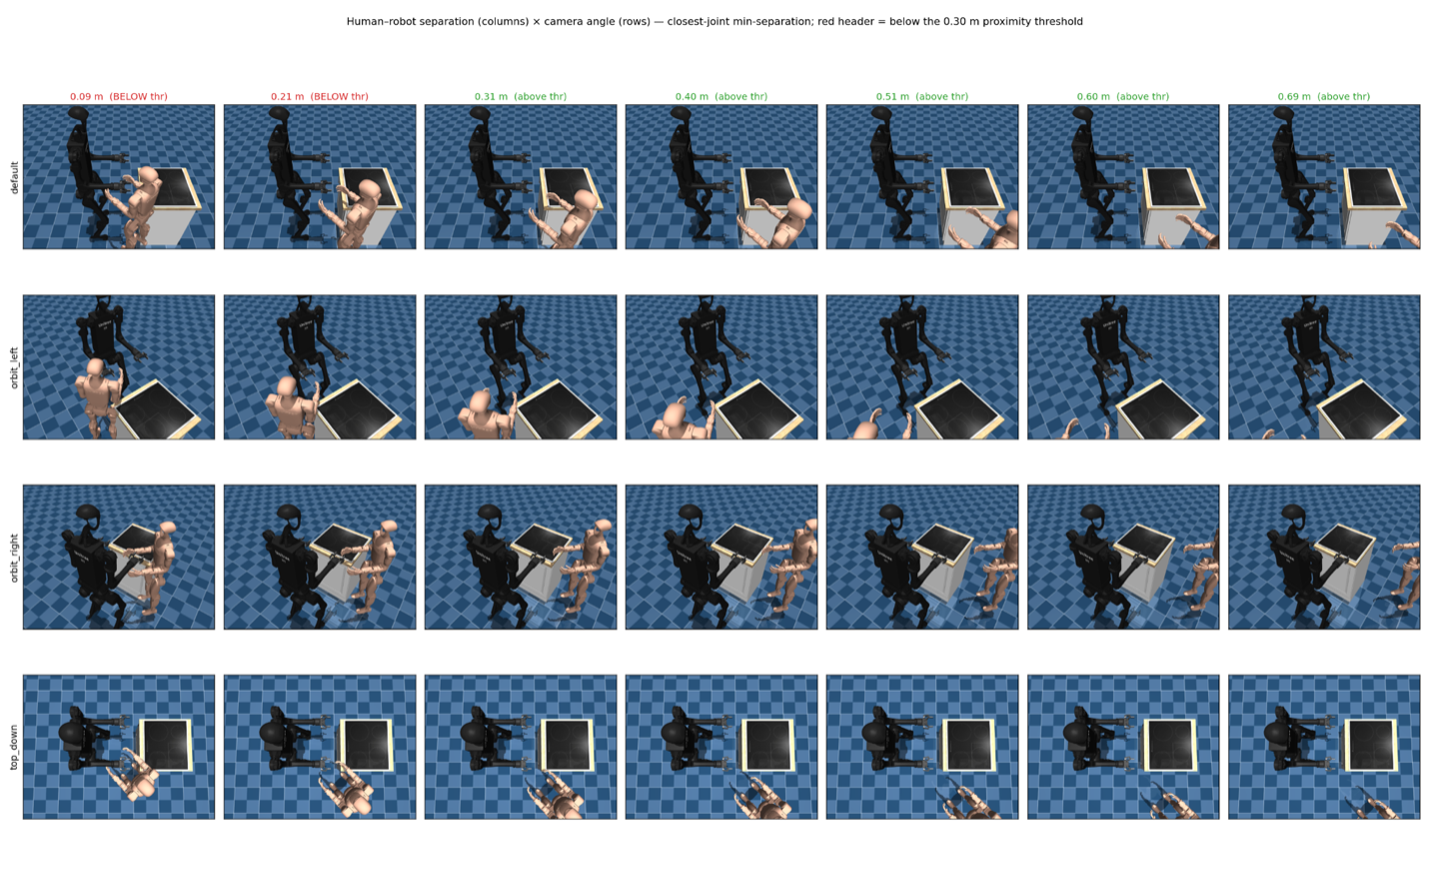
\includegraphics[width=0.62\textwidth]{separation_render_grid.png}
\caption{Contact-geometry calibration of $\tau_{\mathrm{prox}}$. The
H1 robot (dark) and the G1 coworker (light) are rendered at seven
controlled closest-joint separations (columns) from four camera angles
(rows), with the \texttt{saucepan\_to\_hob} table between them. Red
column headers are below the $0.30$\,m proximity threshold: at $0.09$
and $0.21$\,m the body geometries visibly interpenetrate, whereas by
$0.31$\,m (green) a clear gap has opened. This confirms that $0.3$\,m
sits just above the physical contact band, so a proximity violation
fires \emph{before} contact, complementing the empirical-CDF knee of
Table~\ref{tab:prox-calib}.}
\label{fig:separation-scale}
\end{figure}

\paragraph{Empirical distribution.}
Because the proximity-violation rate at threshold $\tau$ is exactly the
empirical CDF $P(\min\text{-separation} < \tau)$, the threshold can be
read off the separation distribution directly. On the G1 stage-2
baseline (3 seeds, 20 episodes, 30{,}000 steps) the distribution is
bimodal, a near-contact mode at 0--0.2\,m plus a far mid-range and
patrol tail, with a knee at $\tau \approx 0.2$--$0.3$\,m
(Table~\ref{tab:prox-calib}); the knee is consistent across two
independently trained policies, so it reflects scene contact geometry
rather than a single controller.

\begin{table}[htbp]
\centering
\small
\caption{Proximity-violation rate as a function of the threshold
$\tau$ (the empirical CDF of $\min$-separation on the G1 stage-2
baseline, 3 seeds $\times$ 20 episodes, 30{,}000 steps). The rate
climbs steeply once $\tau$ crosses into the benign mid-range, which is
why a $0.5$\,m or $1.0$\,m threshold would absorb a large benign
population.}
\label{tab:prox-calib}
\begin{tabular}{lccccccc}
\toprule
$\tau$ (m) & 0.20 & \textbf{0.30} & 0.40 & 0.50 & 0.60 & 0.75 & 1.00 \\
\midrule
Violation rate & 20.1\,\% & \textbf{25.3\,\%} & 29.9\,\% & 35.8\,\% & 39.5\,\% & 47.0\,\% & 62.9\,\% \\
\bottomrule
\end{tabular}
\end{table}

We fix $\tau_{\mathrm{prox}} = 0.3$\,m: it sits at the knee, $\sim$0.2\,m
above the contact band, and captures the genuine near-contact
population without absorbing the benign mid-range proximity that a
$0.5$\,m ($36\,\%$) or $1.0$\,m ($63\,\%$) threshold would. Being
purely geometric it is speed-independent, so the proximity-violation
rate is comparable across policies, tasks and disruption bands, and
it is held fixed across every experiment in this report. The
$\approx$25\,\% near-contact rate this calibration rollout induces
is precisely the behaviour the constrained policy and the runtime
filters are meant to reduce (the headline benchmark reports $0.296$
for the same baseline under per-episode aggregation,
Table~\ref{tab:e4.1-feature-incremental}).

\section{Continuous Cost Signals}
\label{sec:bench:cost}

The wrapper computes two continuous, anticipatory cost signals from
the \iso{} margins:
\begin{align}
  c^{\ssm}_t  &= \max\!\left(0,\; 1 - \frac{m^{\ssm}_t}{d_{\mathrm{buffer}}}\right),
    \label{eq:c-ssm} \\
  c^{\pfl}_t  &= \max\!\left(0,\; f^{\mathrm{ratio}}_t - 0.8\right),
    \label{eq:c-pfl} \\
  c_t         &= \min\!\left(1,\; \max(c^{\ssm}_t,\, c^{\pfl}_t)\right),
    \label{eq:c-total}
\end{align}
where $m^{\ssm}_t$ is the instantaneous \ssm{}-actual margin
(positive when safe, negative when violating), $d_{\mathrm{buffer}}
= 0.3$\,m is the anticipation buffer, and $f^{\mathrm{ratio}}_t$ is
the force-ratio from Equation~\ref{eq:iso-pfl-ratio}. The
aggregator takes the worst-case across both criteria and saturates
at $c_t = 1$.

\paragraph{Why continuous rather than binary.}
A binary indicator $c_t \in \{0,1\}$ on violation supplies only
\emph{post-hoc} gradient signal. The policy learns that crossing
the threshold is bad but receives no information about how close to
the threshold it is approaching. The continuous formulation in
Equations~\ref{eq:c-ssm}--\ref{eq:c-pfl} gives a non-zero cost
before violations occur: a \ssm{}-actual margin of $0.15$\,m carries
a cost of $\sim$0.5, and any margin beyond the $0.3$\,m buffer
carries zero. We adopt it for this gradient richness. We note in
advance, however, that the cost-signal \emph{form} turns out
\emph{not} to be the operative variable: Experiment~E3.1
(Section~\ref{sec:results:cost-signal}) shows that at a tight budget
both the continuous and the binary forms collapse, because the
binding quantity is the Lagrangian budget relative to the task's
inherent cost, not the encoding of the cost. The continuous form is
retained as the more principled design, not because it is shown to
dominate the binary one.

The choice of $d_{\mathrm{buffer}} = 0.3$\,m matches the typical
\iso{}~\ssm{} robot-stopping contribution at the H1's observed
end-effector speeds; the 0.8 threshold in Equation~\ref{eq:c-pfl}
matches the 20\,\% headroom that \iso{} Annex~A motivates for
``approaching the limit''.

\paragraph{The \pfl{} contact-detection limitation.}
\pfl{} flag computation reads MuJoCo's \texttt{data.ncon} for
human--robot contact pairs. \bigym{}'s runtime robot-attachment in
\textsc{mojo} currently produces \texttt{data.ncon = 0} for these
pairs despite geometric overlap, so $c^{\pfl}_t \equiv 0$ throughout
the project. The wrapper exposes a \texttt{use\_pfl} flag wired
through every component; the flag can be flipped on once the
contact-detection issue is resolved without architectural change.
\textbf{All quantitative compliance claims in this report are
qualified as \ssm{}/proximity-only}
(Section~\ref{sec:disc:pfl-bug}).

\section{The \coworker{} Disruption: Design and Rationale}
\label{sec:bench:coworker}

The dominant deployment pattern for human-aware manipulation is
\emph{sustained co-working}: the human is in the workspace for the
whole task, not for a one-shot intrusion, which is the situation a
household robot in a kitchen actually faces. The original \bigym{}
distribution had no human at all, and the legacy disruption types in
the \sbigym{} ecosystem all encoded a single intrusion event per
episode, inadequate as a training distribution for this setting. We
introduce \textsc{Disruption.coworker} as the primary distribution
for both training and evaluation.

\subsection{Design Goals}
\label{sec:bench:coworker:design}

The \coworker{} disruption was designed against three concrete
targets:

\begin{enumerate}[topsep=2pt,itemsep=2pt]
\item \emph{Realism.} The human's behaviour should resemble what a
  real co-worker would do in a shared kitchen: enter the workspace,
  approach the task area, occasionally reach toward the task object
  or toward the robot's own arm, and occasionally step
  away for a moment. Episodes should feel like minutes of
  collaboration, not seconds of intrusion.
\item \emph{Sufficient disruption to expose unsafe behaviour.} If
  the human's reaches are rare or always far from the robot, a
  fast-but-careless policy is safe by luck and the benchmark cannot
  discriminate. The \coworker{} band tightens the closest
  \emph{pelvis-to-pelvis} approach (0.60--0.95\,m) and the
  \textsc{near} dwell (9--14\,s); the reaching arm extends well
  inside the body-centre separation, so the closest geometry pair
  routinely enters the $\tau_{\mathrm{prox}} = 0.3$\,m zone. The
  resulting baseline
  \texttt{ep\_proximity\_violation\_rate} of $0.296$
  (Section~\ref{sec:results:baseline}) is high enough to expose a
  $20+\,\%$ improvement as statistically significant.
\item \emph{Compositional disruption modes.} A real co-worker
  exhibits at least three distinct behaviours over a session:
  staying put while reaching; walking in then staying; walking in,
  leaving briefly, and returning. The \coworker{} sampler covers all
  three but weights them unequally, drawing the most demanding mode
  (patrol) the large majority of the time so that the training
  distribution concentrates on the hardest behaviour while still
  exercising the simpler ones.
\end{enumerate}

\subsection{Three Trajectory Modes}
\label{sec:bench:coworker:traj}

A \coworker{} scenario samples one of three trajectory modes, with
the patrol mode drawn $\sim$90\,\% of the time and the two simpler
modes sharing the remaining $\sim$10\,\%:

\begin{description}[leftmargin=2em,topsep=2pt,itemsep=2pt]
\item[\textsc{stationary}] G1 spawns at \textsc{near} distance and
  stays put. Arm reaches throughout the episode.
\item[\textsc{approach-loiter-depart}] G1 spawns far, walks in to
  \textsc{near}, stays put. Arm reaches after arrival.
\item[\textsc{coworker-patrol}] G1 walks in to \textsc{near}, then
  cyclically departs to an \textsc{away} position (90°--270°
  offset, $\sim$2--3\,m), loiters, returns to a \emph{new}
  \textsc{near} position (different angle, slightly different
  distance), and repeats. Arm reaches only while at \textsc{near}.
\end{description}

The patrol mode is the most realistic operational pattern and is
therefore the dominant mode at full strength; the two simpler modes
are retained both as occasional variety in the headline distribution
and as the bulk of the earlier curriculum stages
(Section~\ref{sec:method:curriculum}), which ramp up to the
patrol-dominant mixture.

\subsection{Arm State Machine and Reach Gate}
\label{sec:bench:coworker:arm}

Independently of trajectory, the G1's reaching arm runs a four-state
cycle, \textsc{extend} $\to$ \textsc{hold} $\to$ \textsc{retract}
$\to$ \textsc{idle} (fractions $0.15/0.20/0.15/0.50$ of a period
$T \in [1.3, 2.2]$\,s in the train band), sampling per cycle whether
to reach for the robot's end-effector or the task object
(\texttt{target\_mix\_p\_ee}), with the target re-resolved each step
so the reach tracks a moving robot. A \emph{reach gate} suppresses
the IK during patrol's \textsc{away} phase. Because the arm idles
half of each cycle and patrol periodically vacates the \textsc{near}
zone, the task remains completable throughout: the success-rate axis
rewards progress in those windows over a trivial ``freeze until the
human leaves'' strategy.

\subsection{Train and Eval Parameter Spaces}
\label{sec:bench:coworker:params}

Five \coworker{} axes are exposed as continuous
\texttt{ParameterSpace} ranges, with train and eval distributions
configured separately for the OOD generalisation experiment (E5.2):

\begin{table}[htbp]
\centering
\small
\caption{The \coworker{} train and eval \texttt{ParameterSpace}.
Train is moderately tight, deliberately set to produce a high
baseline violation rate (so a $20+\,\%$ safety improvement is
statistically detectable). Eval is wider, capturing the
generalisation question. The 0.60\,m closest-approach floor is the
smallest body distance that keeps the G1 mocap-pelvis collision
capsule clear of the H1 pelvis collision capsule; tighter values
generate spurious contact forces and are pathological.}
\label{tab:coworker-params}
\begin{tabular}{lcc}
\toprule
Axis & Train (\texttt{coworker\_train}) & Eval (\texttt{coworker\_eval}) \\
\midrule
Closest-approach distance     & $0.60$--$0.95$\,m  & $0.6$--$1.8$\,m  \\
Reach period $T$              & $1.3$--$2.2$\,s    & $3.0$--$9.0$\,s  \\
$P(\text{reach EE})$          & $0.45$--$0.72$     & $0.1$--$0.9$     \\
Near-loiter dwell time        & $9.0$--$14.0$\,s   & $4$--$16$\,s     \\
Walk speed                    & $1.0$--$1.4$\,m/s  & $0.6$--$2.2$\,m/s\\
\bottomrule
\end{tabular}
\end{table}

\section{The Task Suite: Three Tasks, Two Co-location Regimes}
\label{sec:bench:task}

The evaluation uses three \bigym{} tasks. \texttt{saucepan\_to\_hob}
is the primary deep-dive task; \texttt{dishwasher\_close} and
\texttt{drawers\_open\_all} complete the suite. The saucepan choice
is motivated by:

\begin{enumerate}[topsep=2pt,itemsep=2pt]
\item \textbf{Long horizon for violation opportunity.}
  \texttt{saucepan\_to\_hob} is a pick-and-place task with a
  vertical clearance constraint; episodes last 30--50\,s, several
  reach cycles of the \coworker{} arm. Shorter reach-target tasks
  end before the coworker has cycled enough to expose representative
  unsafe behaviour.
\item \textbf{Workspace overlap with the coworker.} The saucepan
  pickup and the hob target are both within the H1's primary
  reach envelope, which is also where the G1 reaches when the
  reach target is the task object. Episode trajectories therefore
  pass through the same volume the coworker occupies, exposing
  real \ssm{} violations rather than incidental closeness.
\item \textbf{\bigym{}-RL competence.} Of the four candidate
  \bigym{} tasks we screened with ACT baselines, \texttt{saucepan\_to\_hob}
  combines the longest horizon with the greatest workspace overlap,
  and the unconstrained \cqnas{} agent
  (Section~\ref{sec:results:baseline}) reaches a strong
  \texttt{success\_rate} on it after the curriculum
  (Section~\ref{sec:method:curriculum}). The unconstrained baseline
  is a non-trivial reference: any safety improvement we report is
  against a competent task policy, not a policy that was failing the
  task anyway. \cqnas{} task-performance on \bigym{} is documented
  in~\cite{seo2024cqnas}.
\end{enumerate}

\paragraph{Two co-location regimes.}
Although all three tasks run under the \emph{same} \coworker{}
disruption distribution, the task geometry and the policy's motion
pattern make the resulting human--robot co-location qualitatively
different, and this difference turns out to be the variable that
governs which safety mechanism works (Chapter~\ref{ch:eval}). On
\texttt{saucepan\_to\_hob} the coworker's reach destination coincides
with the robot's working volume for most of the episode: the
co-location is \emph{persistent}, with the closest geometry pair
inside the interaction envelope nearly continuously. On
\texttt{dishwasher\_close} and \texttt{drawers\_open\_all} the close
encounters arrive in \emph{bursts}, the coworker's patrol cycle and
the appliance-facing geometry leave genuinely-safe windows between
approaches: co-location is \emph{intermittent}. We do not assert this
distinction from task descriptions alone; it is \emph{measured} in
Section~\ref{sec:results:boundary} via the activity rate of a
separation-triggered runtime filter, which is the operational
definition used throughout (persistent $\approx$ the filter would be
active most of the time; intermittent $\approx$ it would not).
Figure~\ref{fig:task-suite} shows the three settings at a
close-approach instant.

\begin{figure}[htbp]
\centering
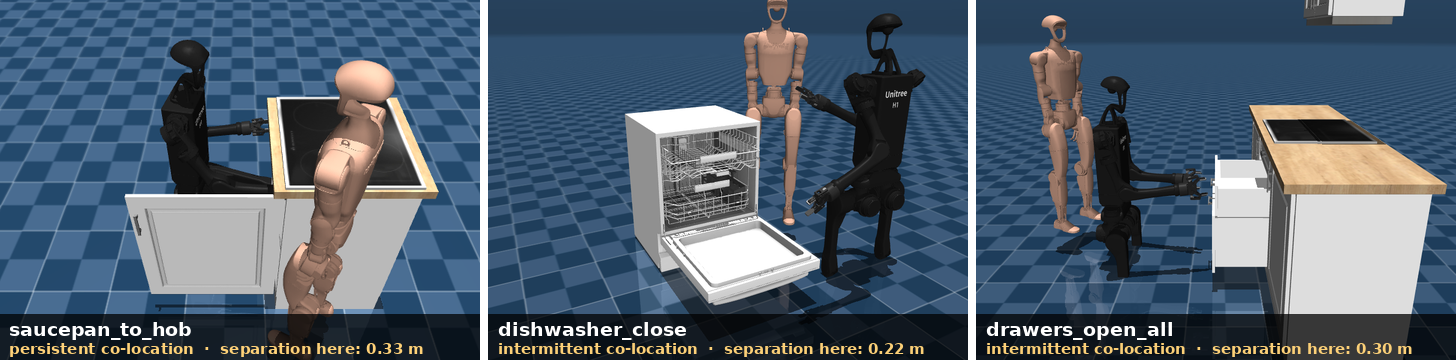
\includegraphics[width=\textwidth]{task_suite}
\caption{The three-task suite, photographed mid-episode from live
task executions under the
\coworker{} disruption: the Unitree H1 manipulator (black) shares
its working volume with the Unitree G1 human-coworker stand-in
(light) in the \bigym{} kitchen. Left: \texttt{saucepan\_to\_hob},
whose pick-and-place trajectory and the coworker's reach destination
coincide, so co-location is \emph{persistent}. Centre and right:
\texttt{dishwasher\_close} and \texttt{drawers\_open\_all}, where
close encounters arrive in bursts separated by genuinely-safe
windows (\emph{intermittent} co-location). The annotated separation
is the environment's ground-truth closest-pair distance at the
pictured instant; the same coworker distribution drives all three
tasks, so the regime is a property of the task--coworker pair, not
of the disruption.}
\label{fig:task-suite}
\end{figure}

\section{Mock \bodyslampp{}: Calibrated Perception Noise}
\label{sec:bench:perception}

Training-time runs use ground-truth human position; deployment-time
runs use a noisy estimate. To characterise the perception
sim-to-real gap, we expose a configurable
\texttt{BodySLAMWrapper} with three modes:

\begin{description}[leftmargin=2em,topsep=2pt,itemsep=2pt]
\item[\texttt{off}] No human-state channel in the observation.
\item[\texttt{oracle}] Ground-truth human position injected as
  \texttt{human\_pos\_estimate} (6D: position + occluded flag +
  staleness counter + confidence).
\item[\texttt{noisy}] The full mock-\bodyslampp{} pipeline, calibrated
  against the published noise characteristics ~\cite{henning2023bodyslampp}.
\end{description}

The noisy pipeline applies, in order:
\begin{enumerate}[topsep=2pt,itemsep=1pt]
\item Ornstein-Uhlenbeck temporally-correlated position noise
  ($\alpha = 0.9$, $\sigma = 0.05$\,m, stationary std $\approx
  0.115$\,m), calibrated against \bodyslampp{}'s reported
  positional accuracy~\cite{henning2023bodyslampp}.
\item 3-step latency buffer ($\approx 60$\,ms at 50\,Hz control,
  matching the 15+\,FPS perception clock typical of monocular
  visual-inertial pose estimation).
\item Stochastic tracking dropout ($p = 0.02$/step) with staleness
  counter; OU state continues to update during dropout, so
  recovery is smooth rather than discontinuous.
\item Optional ray-cast occlusion from the H1's head camera
  (opt-in).
\end{enumerate}

\paragraph{Demo-replay path.}
Cached \bigym{} demonstrations~\cite{chernyadev2024bigym} were
recorded \emph{without} a coworker; their
\texttt{human\_pos\_estimate} would be missing if read live. The
wrapper supports a \texttt{mode=demo\_replay} path that synthesises
\texttt{human\_pos\_estimate} from an
\texttt{AMASSDemoPositionProvider}~\cite{mahmood2019amass} playing
back a real motion clip, so a behaviour-cloning pretraining phase
sees realistic human state at training time without a train→eval
distribution shift on the channel.

\section{Demonstrations and the Demo-Conversion Pipeline}
\label{sec:bench:demos}

\cqnas{}~\cite{seo2024cqnas} is a demo-driven RL agent
($\text{num\_demos} > 0$ assumed at construction); demo-free runs on
long-horizon manipulation never discover the sparse reward and
collapse to workspace evacuation. The demo path uses the raw,
non-safety-wrapped \bigym{} environment to match
\texttt{DemoStore}'s class-name lookup, fetches 10--36 cached
demonstrations, and converts each to \texttt{ExtendedTimeStep}s
carrying the synthesised \texttt{human\_pos\_estimate} channel and a
safe-side placeholder $c_t = 0$ (the cached demos contain no live
human; the curriculum of Section~\ref{sec:method:curriculum} makes
this benign in practice). The most consequential of the
action-normalisation pitfalls fixed during integration
(Section~\ref{sec:impl:integration}): \cqnas{}'s normalisation must
use \emph{demo-derived} action statistics so the live and demo
distributions share a binning.
% =============================================================================
% PART III: A HYBRID SAFETY ARCHITECTURE (the solution)
% =============================================================================

% =============================================================================
\chapter{Methods: The Two Arms of the Hybrid Safety Critic}
\label{ch:method}
% =============================================================================

\section{Overview: Two Arms, One Open Question}
\label{sec:method:overview}

Chapter~\ref{ch:benchmark-env} introduced \sbigym{} as the
benchmark and Section~\ref{sec:bench:why} listed six concrete
properties the benchmark is designed to test. The unconstrained
\cqnas{}~\cite{seo2024cqnas} baseline that ships with \bigym{}
fails almost all six: it has no representation of human position,
no \ssm{} margin, no constraint that would distinguish a
task-completing trajectory from one that endangers the coworker,
and Section~\ref{sec:results:baseline} will show that it registers
proximity violations on $\approx$30\,\% of steps (mean separation only
$0.13$\,m, with the worst approaches within a few millimetres), far
above what any plausible co-working deployment would accept.

This chapter presents \textbf{our solution to that gap}: the Hybrid
Safety Critic, a two-arm safety architecture that turns the
unconstrained imitation-or-RL policy into an \iso{}-aware
collaborator. The architecture has two mechanisms with deliberately
different roles:

\begin{enumerate}[topsep=2pt,itemsep=2pt]
\item A \textbf{training-time mechanism} that \emph{internalises}
  safety into the policy via a value-based Lagrangian formulation
  of the continuous cost signal. At deployment, the policy is
  used as-is; the safety knowledge is baked into the learned
  $Q$-functions (Section~\ref{sec:method:lagrangian}).
\item A \textbf{deployment-time mechanism}: a runtime \emph{filter
  slot} that intercepts the policy's proposed actions. The slot is
  mechanism-agnostic, and we specify and evaluate the complete
  reactive taxonomy through it: an offline-trained, frozen safety
  value function (SVF) used as a veto, the original design
  (Section~\ref{sec:method:filter}); two closed-form
  alternatives, a graded \iso{} speed-scaling rule and a model-based
  geometric dodge (Section~\ref{sec:method:filter:closedform}); and
  the \emph{critic-gated speed-scaling} combination, the SVF deciding
  \emph{when} to intervene and the graded scaler deciding \emph{how}
  (Section~\ref{sec:method:filter:gated}), which is the Hybrid Safety
  Critic's runtime arm.
\end{enumerate}

Both mechanisms share a network shape and an observation interface,
which keeps the two safety critics directly comparable and leaves SVF
reuse available as an option, though the constrained policy's cost
critic is in fact cold-started
(Section~\ref{sec:method:lagrangian:warmstart}); they differ in
training objective and operational role. The full pipeline at
deployment is sketched in Figure~\ref{fig:hybrid-overview}. One
question is deliberately left open in this chapter: \emph{which arm
should carry the safety burden in a given deployment}. That is the
empirical question the thesis answers, and the chapters that follow
answer it with the regime map rather than presupposing either arm.

\begin{figure}[htbp]
\centering
\resizebox{\textwidth}{!}{%
\begin{tikzpicture}[
  >=Latex, node distance=10mm and 11mm,
  box/.style={draw, rounded corners, align=center, inner sep=4pt,
              minimum height=11mm, font=\small},
  env/.style={box, fill=black!5},
  pol/.style={box, fill=blue!8, draw=blue!55, minimum width=42mm},
  filt/.style={box, fill=orange!12, draw=orange!70, minimum width=34mm},
  trn/.style={box, dashed, fill=black!3, draw=black!45, align=center,
              font=\footnotesize, text=black!75, minimum height=10mm},
  flow/.style={->, thick},
  tflow/.style={->, thick, dashed, black!55},
]
% deployment row
\node[env] (env) {Environment\\[-1pt]{\footnotesize \textsc{BiGym} $+$ G1 coworker}};
\node[box, right=of env] (obs) {Observation $s_t$\\[-1pt]{\footnotesize proprio.\ $+\ \hat p_{\mathrm{human}}$}};
\node[pol, right=of obs] (pol) {Policy $\pi$\\[2pt]$a^{\mathrm{nom}}=\mathrm{argmax}_{a}[\,Q_r-\lambda Q_c\,]$};
\node[filt, right=of pol] (filt) {Runtime filter\\[2pt]$Q_{\mathrm{safe}}(s,a^{\mathrm{nom}})\ge R$\,?};
\node[box, right=of filt] (exec) {Execute $a_t$};

\draw[flow] (env) -- (obs);
\draw[flow] (obs) -- (pol);
\draw[flow] (pol) -- (filt);
\draw[flow] (filt) -- node[above,font=\footnotesize]{pass}
                      node[below,font=\footnotesize]{$a_t{=}a^{\mathrm{nom}}$} (exec);

% veto branch
\node[box, fill=orange!5, draw=orange!55, font=\footnotesize,
      minimum height=8mm, below=9mm of filt] (fb) {fallback $a^{\mathrm{fb}}$};
\draw[flow] (filt.south) -- node[right,font=\footnotesize]{veto} (fb.north);
\draw[flow] (fb.east) -| (exec.south);

% feedback loop
\draw[flow] (exec.north) -- ++(0,7mm) -| (env.north);

% training band
\node[trn, below=15mm of pol] (lag)
  {trained \emph{online}: value-based\\ Lagrangian on cost $c_t$
   $\;\Rightarrow\; Q_r,Q_c$};
\node[trn, below=15mm of fb] (cql)
  {trained \emph{offline} (CQL),\\ frozen at deployment
   $\;\Rightarrow\; Q_{\mathrm{safe}}$};
\draw[tflow] (lag) -- (pol);
\draw[tflow] (cql.north) -- (filt.west);
\end{tikzpicture}%
}
\caption{The Hybrid Safety Critic at deployment: a two-arm
architecture. At each step the Lagrangian-trained policy proposes the
nominal action
$a^{\mathrm{nom}} = \mathrm{argmax}_a\,[Q_r(s,a) - \lambda Q_c(s,a)]$;
a runtime filter slot passes it through when its safety check holds
and otherwise modifies or replaces it (veto, dodge, graded
speed-scaling, or critic-gated speed-scaling,
Sections~\ref{sec:method:filter}--\ref{sec:method:filter:gated}). The
two arms have deliberately different jobs: the constrained policy
internalises safety \emph{proactively} during training, while the
filter is a \emph{reactive} runtime mechanism. Chapter~\ref{ch:eval}
shows that which arm carries the safety burden is governed by the
co-location regime: under persistent co-location only the policy
reduces exposure gracefully
(Table~\ref{tab:e4.1-feature-incremental}), while under intermittent
co-location the critic-gated filter is the working arm
(Section~\ref{sec:results:r2-gated}).}
\label{fig:hybrid-overview}
\end{figure}

\section{The Offline Safety Value Function}
\label{sec:method:filter}

\subsection{Dataset and Labelling}
\label{sec:method:filter:data}

The SVF is trained offline on a dataset of transitions collected by
rolling out \cqnas{} policy snapshots from the base-policy curriculum
(Section~\ref{sec:method:curriculum}) in the \coworker{} distribution
under the \texttt{noisy} observation mode. Earlier iterations of the
critic mixed random-policy and demonstration transitions; the current
critic is collected from policy snapshots alone. The reasoning is that
the regions a deployed policy actually visits are precisely the regions
the filter must judge accurately, and snapshot rollouts sample exactly
that on-policy distribution, including the imitation-learning artefacts
a competent-but-imperfect policy exhibits under sustained co-working
disruption. The filter is \emph{noisy-native}: it is trained and
evaluated on \texttt{noisy} human-state estimates, and on
ground-truth (\texttt{oracle}) input its $Q$-estimates collapse and it
intervenes almost everywhere, so all filtered evaluations are reported
on \texttt{noisy} (Section~\ref{sec:setup:perception-mode}). The exact
transition count for the current critic is 37{,}883, of which
$16.8\,\%$ are labelled unsafe ($r^{\mathrm{safe}} = 0$) at the
$\tau = 0.3$\,m proximity threshold; the full figures are in the
repository's filter-training write-up.

Each transition is labelled with the binary safety reward
\begin{equation}
  r^{\mathrm{safe}} \;=\; 1 - \mathbb{1}[\texttt{proximity\_violation}],
  \label{eq:r-safe}
\end{equation}
using the geometric proximity-violation flavour of
Section~\ref{sec:bench:metrics:flavours} at the calibrated threshold
$\tau_{\mathrm{prox}} = 0.3$\,m (the calibration is derived in
Section~\ref{sec:bench:proximity-threshold}). We label on
\texttt{proximity\_violation} rather than \texttt{ssm\_violation\_actual}
for two reasons. First, the conservative-ISO \ssm{} flag is saturated:
it fires on $\sim$93\,\% of random rollouts and remains high even for
competent policies because it assumes the worst-case human velocity, so
it carries almost no gradient for a value function to learn. Second, and
by design, labelling on geometry keeps a clean separation of concerns
between the two safety mechanisms. The runtime filter is made
responsible for the \emph{geometric} danger of being too close, while
the velocity-dependent \ssm{} response is left to the cost signal and
the constrained policy (Section~\ref{sec:method:lagrangian}). Coupling
the filter's training target to instantaneous velocity would make its
label depend on the very action it is meant to veto, conflating ``how
dangerous is this configuration'' with ``how fast is the robot moving'',
the latter being a decision the policy, not the filter, should own.

Because the violating class is the minority, a
\texttt{WeightedRandomSampler} over-samples it to a $1{:}1$ ratio of
safe to violating transitions per batch, so the critic is not
dominated by the safe majority.

\paragraph{A second, task-agnostic critic for the intermittent-co-location tasks.}
The same pipeline produces the critic used on
\texttt{dishwasher\_close} and \texttt{drawers\_open\_all}: a single
shared SVF trained once on 52{,}794 transitions collected from
curriculum-policy rollouts on both tasks under \coworker{}
disruption, labelled by geometric \emph{near-contact}
($\min$-separation $< 0.10$\,m). The observation specification
(proprioception $+$ human-position estimate $+$ action) is identical
across the two tasks, so one critic serves both, evidence that the
learned safety signal is task-agnostic at matching embodiment. The
tighter $0.10$\,m label (versus the saucepan critic's $0.30$\,m) makes
this critic a \emph{near-contact} detector rather than a proximity
detector; an ablation with looser, earlier-warning labels ($0.20$ /
$0.30$\,m) confirms the selective near-contact label is the better
gate (Section~\ref{sec:results:r2-ablations}).

\subsection{Architecture and Training}
\label{sec:method:filter:arch}

The safety critic is a 3-layer MLP with hidden sizes
$[256, 256, 256]$ and ReLU activations. The input is the
concatenation of robot proprioception, the mock-\bodyslampp{} 6D
human-position estimate, and the proposed action. The output is
bounded to $[0, q_{\max}]$ with $q_{\max} = 1/(1-\gamma)$ via a
scaled sigmoid, which \emph{mathematically} prevents Bellman
overestimation: $Q$ cannot exceed the maximum possible discounted
return of a safe trajectory.

Training combines a Bellman residual with the
\textsc{CQL}~\cite{kumar2020cql} regulariser:
\begin{equation}
  \mathcal{L} \;=\; \mathcal{L}_{\mathrm{Bellman}}
  \;+\; \alpha_{\mathrm{CQL}} \cdot
  \left(\mathbb{E}_{a \sim \mathrm{uniform}}\!\left[Q(s,a)\right]
       - \mathbb{E}_{a \sim \mathcal{D}}\!\left[Q(s,a)\right]\right),
  \label{eq:cql-loss}
\end{equation}
with $\alpha_{\mathrm{CQL}} = 5.0$ as the headline value, Polyak
target update $\tau = 0.005$. Full training hyperparameters in
Appendix~\ref{app:hparams:svf}.

\subsection{No-Pixel Critic: Justification}
\label{sec:method:filter:nopixels}

The filter does not consume RGB, for three reasons: \emph{compute}
(a pure-MLP critic costs $\sim$0.3\,ms per forward against a
$\sim$20\,ms control budget, versus a substantial CNN-encoder
fraction); \emph{robustness} (no lighting/texture domain shift, only
the upstream pose estimator's
calibration~\cite{henning2023bodyslampp}); and
\emph{compositionality} (a no-pixel filter wraps any policy whose
observation includes proprioception, the human-position estimate,
and the proposed action).

\subsection{Runtime Wrapper}
\label{sec:method:filter:runtime}

At deployment, the \texttt{SafetyFilterWrapper} intercepts the
proposed action and compares the safety value against a threshold
$R$:
\begin{equation}
  a^{\mathrm{exec}}_t \;=\;
  \begin{cases}
    a^{\mathrm{nom}}_t   & \text{if } Q_{\mathrm{safe}}(s_t, a^{\mathrm{nom}}_t) \ge R, \\
    a^{\mathrm{fb}}_t    & \text{otherwise.}
  \end{cases}
  \label{eq:filter-rule}
\end{equation}
$R$ is calibrated by sweep over a held-out validation set
(Experiment~E2.3, Section~\ref{sec:results:filter-pareto}); the
headline operating point for the G1 critic on the \coworker{}
distribution is $R = 2.25$. The intended role of the veto at this
operating point is an \iso{}~\ssm{} \emph{velocity backstop} rather
than a proximity reducer: much of the residual proximity is the
human walking up to an otherwise stationary robot, which no veto of
robot actions can prevent; Section~\ref{sec:results:filter-pareto}
quantifies the resulting limits.

The veto's fallback is zero-velocity braking on the floating base
and on every joint velocity actuator. This can produce abrupt
motion mid-trajectory; proportional damping is the natural upgrade
and is deferred to future work (Section~\ref{sec:fw:fallback}).

\section{Closed-Form Runtime Filters: Speed-Scaling and Geometric Dodge}
\label{sec:method:filter:closedform}

The filter slot of Figure~\ref{fig:hybrid-overview} is
mechanism-agnostic: anything that maps the state and the proposed
action $(s_t, a^{\mathrm{nom}}_t)$ to an executed action can occupy
it. The learned SVF veto above is its learned instantiation. Two
\emph{closed-form} mechanisms, specified here and evaluated alongside
the veto in Chapter~\ref{ch:eval}, complete the reactive taxonomy:
stop (veto), slow (speed-scaling), and move away (dodge). Both
consume the same $\hat{p}^{\mathrm{human}}$ estimate as the SVF and
contain no learned component.

\subsection{Graded \iso{} Speed-Scaling}
\label{sec:method:filter:speedscale}

\iso{}~\ssm{}'s intent is graded: the robot should \emph{slow} as
separation shrinks, not merely stop at a threshold. The speed-scaling
filter implements this directly. At each step a scale factor is
computed from the closest-pair human--robot separation
$\mathrm{sep}_t$,
\begin{equation}
  \sigma_t \;=\; \mathrm{clip}\!\left(
    \frac{\mathrm{sep}_t - d_{\mathrm{stop}}}
         {d_{\mathrm{slow}} - d_{\mathrm{stop}}},\; 0,\; 1\right),
  \qquad
  a^{\mathrm{exec}}_t \;=\; q_t + \sigma_t \,
    \bigl(a^{\mathrm{nom}}_t - q_t\bigr),
  \label{eq:speed-scale}
\end{equation}
where $q_t$ is the current joint position for the absolute-mode arm
dimensions (so the per-step \emph{motion} from the current pose is
scaled) and zero for the delta-mode floating base (so the commanded
increment is scaled directly). Above $d_{\mathrm{slow}}$ the filter
is the identity ($\sigma_t = 1$, the action is unchanged); at or
below $d_{\mathrm{stop}} = 0.15$\,m the robot holds position
($\sigma_t = 0$); in between, speed falls linearly with separation.
The slow radius $d_{\mathrm{slow}}$ is the single operating-point
knob, swept over $[0.25, 0.60]$\,m with the headline at $0.40$\,m;
an intervention is any step with $\sigma_t < 1$. Unlike the veto,
this filter preserves the \emph{direction} of the policy's motion
and modulates only its magnitude, which is why it can maintain the
graded velocity margin the standard prescribes where a binary
stop-or-go veto cannot
(Section~\ref{sec:results:headline-feature-table}).

\subsection{Model-Based Geometric Dodge}
\label{sec:method:filter:dodge}

The second closed-form mechanism is a geometric
control-barrier-style fallback: when the closest-pair separation
falls below a target $d_{\mathrm{target}}$, the filter adds a
correction step directed \emph{away} from the human, proportional to
the violation depth $(d_{\mathrm{target}} - \mathrm{sep}_t)$ and
capped per step. Two variants differ in which part of the robot
dodges: the \emph{base-dodge} pushes the floating base along the
escape direction and leaves the arm untouched, while the
\emph{end-effector retract} (``flinch'') keeps the base planted and
retracts the end-effector along the escape direction via a
damped-Jacobian step. $d_{\mathrm{target}}$ is swept over
$[0.30, 0.55]$\,m. These variants exist to test whether a
\emph{dodging} reactive response escapes the limits of the
\emph{stopping} one; Section~\ref{sec:results:reactive-taxonomy}
shows it does not (it trades the veto's freeze for a flee). The
veto and the dodges are reported as taxonomy points
(Table~\ref{tab:filter-taxonomy}), with operating-point values for
all mechanisms in Appendix~\ref{app:hparams:hybrid}.

\subsection{Critic-Gated Speed-Scaling: The Hybrid Safety Critic's Runtime Arm}
\label{sec:method:filter:gated}

The unconditional speed-scaler of
Section~\ref{sec:method:filter:speedscale} pays its task cost at
\emph{every} close approach, including those where the situation is
genuinely safe (the human is close but stationary, or moving away,
or the robot is barely moving). The learned SVF of
Section~\ref{sec:method:filter} knows the difference; the binary veto
is simply the wrong way to act on that knowledge. The
\emph{critic-gated speed-scaling} filter splits the decision:

\begin{equation}
  a^{\mathrm{exec}}_t \;=\;
  \begin{cases}
    a^{\mathrm{nom}}_t
      & \text{if } Q_{\mathrm{safe}}(s_t, a^{\mathrm{nom}}_t) \ge R
        \quad\text{(critic says safe: full speed)}, \\
    q_t + \sigma_t\,(a^{\mathrm{nom}}_t - q_t)
      & \text{otherwise}
        \quad\text{(critic flags risk: graded slow-down, Eq.~\ref{eq:speed-scale})}.
  \end{cases}
  \label{eq:gated-rule}
\end{equation}

The critic decides \emph{when} to intervene; the speed-scaler decides
\emph{how}. Both halves matter. Replacing the graded
slow-down with a hard veto breaks the action coherence of a chunked
policy (Section~\ref{sec:results:r2-veto}); removing the gate makes
the scaler fire on every close approach and pay the full
unconditional task cost. The gate threshold $R$ is the single
operating-point dial: $R \to 0$ recovers the unfiltered policy,
$R \to \infty$ recovers unconditional scaling, and intermediate
values trace a frontier between them
(Section~\ref{sec:results:r2-gated}). Whether that frontier
\emph{bends} toward a high-success/low-violation corner or merely
\emph{slides} between its two endpoints is precisely the
regime-dependent question answered in
Section~\ref{sec:results:boundary}.

\section{The Value-Based Lagrangian Constrained Policy}
\label{sec:method:lagrangian}

\subsection{Why Value-Based}
\label{sec:method:lagrangian:why}

\cqnas{}~\cite{seo2024cqnas} is \emph{critic-only}: the policy is
implicit, $\pi(s) = \mathrm{argmax}_{a \in
\mathcal{A}_{\mathrm{bin}}} Q(s, a)$, over a coarse-to-fine
discretisation of the joint action space. The classical
actor-critic Lagrangian formulation~\cite{ray2019safetygym,
stooke2020pid} updates a policy network $\pi_\theta$ to maximise
$\mathbb{E}[Q_r(s,a)] - \lambda \mathbb{E}[Q_c(s,a)]$, which
presumes that $\pi_\theta$ exists as a separately-trained network.
There is no $\pi_\theta$ in \cqnas{}. The Lagrangian must be
re-expressed in value-based form.

The starting point is the constrained objective
\begin{equation}
  \max_{\pi} J_r(\pi)
  \quad \text{s.t.} \quad
  J_c(\pi) \le d,
  \qquad
  J_r(\pi)=\mathbb{E}_{\pi}\!\left[\sum_t \gamma^t r_t\right],
  \quad
  J_c(\pi)=\mathbb{E}_{\pi}\!\left[\sum_t \gamma^t c_t\right].
  \label{eq:cmdp-objective}
\end{equation}
For any fixed multiplier $\lambda \ge 0$, the Lagrangian relaxation is
$\mathcal{L}(\pi,\lambda)=J_r(\pi)-\lambda(J_c(\pi)-d)$. The
$\lambda d$ term is constant with respect to action choice, so a
critic-only policy can implement the same trade-off at decision time
by learning separate action-values
\[
Q_r(s,a)\approx\mathbb{E}\!\left[\sum_t\gamma^t r_t\mid s_0=s,a_0=a\right],
\qquad
Q_c(s,a)\approx\mathbb{E}\!\left[\sum_t\gamma^t c_t\mid s_0=s,a_0=a\right],
\]
and selecting the action that maximises $Q_r-\lambda Q_c$. This is the
key reproducibility point: \emph{the policy improvement step is changed,
not the Bellman target of the reward critic}. The reward and cost
critics can therefore be trained on stationary targets, while
$\lambda$ acts only as a deployment-time or training-time selection
parameter.

Three options were considered, in increasing principledness; the
choice is itself an empirical comparison
(Experiment~E3.1).

\subsection{Option A-value: Shaped-Reward Single Critic}
\label{sec:method:lagrangian:A}

The simplest re-formulation folds the cost into a modified reward
and trains a single critic:
\begin{equation}
  r^{\mathrm{mod}}_t \;=\; r^{\mathrm{task,shaped}}_t \;-\; \lambda \cdot c_t,
  \qquad
  Q(s,a) \approx \mathbb{E}\!\left[\sum_t \gamma^t r^{\mathrm{mod}}_t\right],
  \label{eq:option-A}
\end{equation}
with action selection $a^* = \mathrm{argmax}_a Q(s,a)$. Its known
pathology: the regression target is \emph{non-stationary} in
$\lambda$, which is itself non-stationary in the rolling cost, so
the critic chases a moving target. Used here as a prototype baseline
only.

\subsection{Option B-value-mean: Dual Q-Functions on Mean Cost (Headline)}
\label{sec:method:lagrangian:Bmean}

Decouple the reward and cost critics:
\begin{align}
  Q_r(s,a) &\approx \mathbb{E}\!\left[\sum_t \gamma^t r^{\mathrm{task,shaped}}_t\right], \\
  Q_c(s,a) &\approx \mathbb{E}\!\left[\sum_t \gamma^t c_t\right],
\end{align}
each regressing toward its own \emph{stationary} target. The action
selection combines them at decision time:
\begin{equation}
  a^* \;=\; \mathop{\mathrm{argmax}}_{a \in \mathcal{A}_{\mathrm{bin}}}
  \Big[\,Q_r(s,a) \;-\; \lambda \cdot Q_c(s,a)\,\Big].
  \label{eq:Bmean-select}
\end{equation}
$\lambda$ now enters only at selection, not at regression. The
cost critic shares its network shape with the offline SVF, so SVF
reuse is available, though here the cost critic is cold-started
(Section~\ref{sec:method:lagrangian:warmstart}). This is the
\textbf{headline architecture} for this work.


\subsection{Option B-value-CVaR: Distributional Cost Critic (future work)}
\label{sec:method:lagrangian:Bcvar}

A natural extension replaces the mean-cost critic with a
distributional one: $Q_c$ is replaced by either a Gaussian
parametrisation $(\mu_c, \sigma_c)$~\cite{yang2021wcsac} or a
quantile head $\{\theta_k\}_{k=1}^K$~\cite{dabney2018qrdqn}, with
action selection
\begin{equation}
  a^* \;=\; \mathop{\mathrm{argmax}}_{a \in \mathcal{A}_{\mathrm{bin}}}
  \Big[\,Q_r(s,a) \;-\; \lambda \cdot \cvar_{\alpha}(Z_c \mid s, a)\,\Big],
\end{equation}
with $\alpha \in \{0.95, 0.99\}$. This would align training with the
\cvar{} evaluation metric and answer the standard critique that
mean-cost methods bound only $\mathbb{E}[Z_c]$; the cost head is
already C51-shaped, but calibrating a rolling-\cvar{} target and
re-verifying the support invariant
(Section~\ref{sec:method:lagrangian:support}) for the cost
distribution is non-trivial engineering. \textbf{We adopt
B-value-mean as the headline and defer explicit-\cvar{} training to
future work (Section~\ref{sec:fw:cvar})}, evaluating the
mean-policy's \emph{achieved} \cvar{} as a diagnostic
(Section~\ref{sec:results:tail}).

\subsection{The C51 Value-Support Invariant}
\label{sec:method:lagrangian:support}

\cqnas{} uses a C51 distributional reward critic with fixed value
support $[v_{\min}, v_{\max}]$~\cite{bellemare2017c51}. The Bellman
target $T_z = r + \gamma \cdot \mathrm{support}$ is clamped to this
support at each update. Adding a dense shaped reward term such as
Equation~\ref{eq:r-workspace} introduces a discounted return whose
value can fall outside the support; once the target is clamped, the
critic loses the ability to distinguish values in the saturating
region, and the gradient that should pull the end-effector back
toward the task is clipped away.

\begin{proposition}[Support-bounding invariant]
\label{lem:support-bound}
Let a C51 distributional critic have value support
$[v_{\min}, v_{\max}]$, discount $\gamma$, and an additive shaped
reward $r^{\mathrm{shaped}}_t \in [-\beta \cdot c_{\mathrm{ws}}, 0]$
with $\beta, c_{\mathrm{ws}} > 0$. The shaped-reward contribution
to the discounted return is bounded by
$\beta \cdot c_{\mathrm{ws}} / (1 - \gamma)$ in magnitude. The
Bellman target clamp is informative (i.e., the support is not
saturated) only if
\begin{equation}
  \beta \cdot c_{\mathrm{ws}} \,/\, (1-\gamma) \;\le\; |v_{\min}|.
  \label{eq:support-invariant}
\end{equation}
\end{proposition}

\begin{proof}
The geometric-series sum of the per-step shaping under the worst
case gives $\sum_{t=0}^\infty \gamma^t \beta c_{\mathrm{ws}} =
\beta c_{\mathrm{ws}} / (1-\gamma)$, and the C51 target clamp
clips below $v_{\min}$. \qed
\end{proof}

\paragraph{Consequence.}
The original workspace shaping ($\beta = 0.2$, no cap on per-step
excess distance) gave a worst-case discounted return of
$-0.2 / 0.01 = -20$ against the default \cqnas{} support of
$[-2, +2]$, saturating every state outside $\sim$0.5\,m of the
task. Training diverged: \texttt{ep\_reward} fell monotonically
from $-78$ to $-775$ over 50k frames as the policy parked further
from the workspace and the support flattened. The fix is
two-sided: cap the per-step penalty ($c_{\mathrm{ws}} = 1.0$\,m),
reduce $\beta$ to 0.05, and widen the support to
$[v_{\min}, v_{\max}] = [-6, +2]$. With these settings the
invariant holds ($0.05 \cdot 1.0 / 0.01 = 5 \le 6$) and training
proceeds normally; the next-attempt \texttt{ep\_reward} reaches
$\sim +1.8$ on stage~1 of the curriculum
(Section~\ref{sec:method:curriculum}).

\textbf{The engineering lesson generalises beyond \sbigym{}.} It
generalises to any distributional critic + dense shaping setting
and applies as a checking principle independent of \sbigym{}.

\subsection{Per-Env-Step Cost Backup}
\label{sec:method:lagrangian:per-step}

\cqnas{} executes \emph{action sequences} of length $K$ between
policy queries (coarse-to-fine refinement). A natural but subtly
wrong design is to backup the cost critic on the chunk-averaged
cost $\bar{c} = (1/K) \sum_{k} c_{t+k}$. The policy can satisfy a
mean-over-chunk budget while spiking violations \emph{inside} a
chunk. The cost critic must be backed up on \emph{every} env-step's
$c_t$. Our training pipeline preserves $c_t$ through the replay
buffer at per-env-step granularity
(Section~\ref{sec:impl:integration}).

\subsection{PID Lagrange Multiplier Update}
\label{sec:method:lagrangian:pid}

The Lagrange multiplier is updated by a PID
controller~\cite{stooke2020pid} on the running constraint violation.
Let $m_t$ be the rolling per-episode cost mean and $d$ the cost
budget; the update is
\begin{align}
  e_t &= m_t - d, \\
  \lambda_{t+1} &= \mathrm{clip}\!\left(\lambda_t + K_I \cdot e_t
    + K_P \cdot e_t + K_D \cdot (e_t - e_{t-1}),
    \; 0,\; \lambda_{\max}\right).
  \label{eq:pid-lambda}
\end{align}
PID is preferred over gradient ascent
($\lambda \leftarrow \lambda + \eta \cdot e_t$) because the
integral term provides faster convergence to the constraint
boundary while the derivative term damps
oscillation~\cite{stooke2020pid}. We use $K_I = 10^{-3}$,
$K_P = 10^{-2}$, $K_D = 0$, and $\lambda_{\max} = 100$. The clamp
prevents the policy from collapsing into a fully-frozen
``safe-and-useless'' attractor when the cost budget is briefly
violated.

\paragraph{PID auto-tuning is seed-unstable at the feasibility
boundary; a fixed multiplier is the fix.}
The task's inherent mean cost is $\approx$0.25--0.30, so any budget
$d \le 0.2$ is infeasible (abandon-the-task is the only policy under
it) and $d = 0.5$ is slack ($\lambda \to 0$); the single viable
budget, $d = 0.3$, sits \emph{at} the inherent cost, where the dual
variable is decided by each seed's stochastic cost trajectory rather
than by design. Across three seeds at $d = 0.3$, $\lambda$ converged
to $0.000$, $0.267$, and $3.855$, unconstrained, graceful, and
windup-collapse respectively; the evidence is presented with the
budget sweep in Section~\ref{sec:results:budget}
(Figure~\ref{fig:lambda-regimes}). The fix is to remove the
auto-tuning: freezing $\lambda$ (zero PID gains, $Q_c$ still trained
and used in dual-action selection) makes all three seeds behave
consistently and turns $\lambda$ into a clean proximity--success
knob; we sweep it and adopt $\lambda = 0.1$ as the headline
($\lambda = 0.27$ over-constrains, $\lambda = 0$ recovers the
baseline; Figure~\ref{fig:fixlam}). The lesson generalises: when the
only feasible budget coincides with the task's inherent cost, the
dual variable carries too little signal to auto-tune, and a fixed or
scheduled multiplier is preferable. The PID path remains in the
codebase as the documented negative.

\subsection{Filter During Training (optional)}
\label{sec:method:lagrangian:filter-train}

The runtime safety filter of Section~\ref{sec:method:filter} can
also be applied at training time, interposed between the proposed
action and the environment, vetoing catastrophically unsafe
proposals with the fallback~\cite{cbfrl2024,shield2025}. We report
results without the training-time filter as the default; the
filter-during-training ablation is deferred to future work
(Section~\ref{sec:fw:filter-during-training}).

\subsection{Cost-Critic Initialisation and Policy Warm-Start}
\label{sec:method:lagrangian:warmstart}

Two initialisation choices matter here, and they point in opposite
directions. The actor, the reward critic and the shared visual encoder
are \emph{warm-started} from the unconstrained base policy: the
stage-1 snapshot of the curriculum
(Section~\ref{sec:method:curriculum}) is loaded so that constrained
training begins from a task-competent policy rather than from scratch.
The cost critic $Q_c$, by contrast, is \emph{cold-started} (freshly
initialised).

This is deliberate. Although $Q_c$ shares its network shape with the
offline SVF, the two carry opposite sign conventions ($Q_c$ high
means dangerous, $Q_{\mathrm{safe}}$ high means safe) and different
learning targets (offline CQL value of a binary proximity label vs.\
online expected value of the continuous cost under the current
policy); seeding $Q_c$ from the SVF would initialise it on a surface
the dual-Q selection step would have to unlearn. A
\texttt{warm\_start\_from\_svf} path (with the required sign-flip)
remains in the codebase, unused in the reported runs. One loader
subtlety matters for reproduction: the unconstrained base
snapshot contains no cost-critic keys, so the loader guards them
explicitly, task weights load, $Q_c$ stays freshly initialised.


\section{External Baseline: Worst-Case SAC}
\label{sec:method:wcsac}

To position the value-based Lagrangian against the published safe-RL
state of the art rather than only against our own ablations, we
faithfully reimplement WCSAC~\cite{yang2021wcsac,yang2023wcsacjournal},
the canonical distributional safe actor-critic, on the same 76-DOF tasks
(\texttt{agent=wcsac} on the same training stack). WCSAC maintains a
Gaussian distributional cost critic and constrains
$\cvar_{\alpha}$ of the discounted cost return ($\alpha = 0.9$) to a
budget $d$ via an adaptively-tuned multiplier. Two faithfulness
points matter. First, WCSAC is actor-critic, so it cannot load the
critic-only \cqnas{} warm-start snapshots; it trains \emph{from
scratch} ($\text{num\_demos} = 0$, 150k frames), which is the honest
configuration and is reported as such, the comparison measures the
published method as a practitioner could actually deploy it on these
tasks, not a demo-warm-started variant that does not exist in the
literature. Second, because it trains demo-free, its action
de-normalisation must use identity statistics; the evaluation harness
originally forced demo-derived statistics onto every snapshot, a
train/deploy mismatch that produced plausible-but-wrong numbers and
was fixed and cross-validated before any WCSAC result was recorded
(the same class of silent confound as
Section~\ref{sec:impl:svf-faithful}). Results in
Section~\ref{sec:results:r2-lagrangian}.

\section{The Base-Policy Curriculum}
\label{sec:method:curriculum}

Direct training on the full \coworker{} disruption distribution
from a randomly-initialised \cqnas{} agent fails. The empirical
signature is a base policy that learns to evacuate the workspace
within 5--10k frames and never attempts the task;
\texttt{ep\_reward} stays at the floor and \texttt{success\_rate}
stays at 0. The cause is a \emph{distribution-shift cascade}:
cached \bigym{} demonstrations contain no coworker, so
behaviour-cloning teaches ``go to the task, ignore everything''; at
runtime, the live coworker physically blocks the task path,
producing off-distribution states; the C51 critic has no reliable
signal in those states and the policy drifts toward whatever
physics + workspace shaping push it toward, which is away from the
human and toward the workspace boundary.

The fix is a three-stage curriculum that resumes from each prior
stage's snapshot~\cite{narvekar2020curriculum}. The environment is
\emph{stateless} with respect to training step, so the curriculum
is implemented as three sequential training runs with snapshot
resume. The \texttt{BodySLAMWrapper} channel and the obs width are
preserved across stages by keeping a coworker in the scene at all
stages (just distant in stage~0), so the architecture and replay
buffer carry over cleanly.

\label{tab:curriculum-stages}%
The three stages are: \emph{stage~0}, \texttt{coworker\_idle} (G1
present but $\sim$3\,m off and never reaching, doubling as a
``can the agent learn the task at all?'' sanity check; 30k frames);
\emph{stage~1}, \texttt{coworker\_easy} (moderate distance,
occasional reaches; 30k); \emph{stage~2}, the full
\texttt{coworker\_train} band of Table~\ref{tab:coworker-params}
(40k). Stages~0--1 saturate well before their budgets; the largest
budget is reserved for the hardest distribution.

\paragraph{Why a curriculum (against alternatives).}
Domain randomisation~\cite{tobin2017domainrand} on the human
velocity from step~0 was considered, but it addresses
dynamics-estimate error, not the actual failure, never discovering
the sparse reward; curriculum learning addresses the discovery
problem~\cite{narvekar2020curriculum,openai2019solving}. The
empirical anchor: stages~0--1 complete with \texttt{ep\_reward}
$\sim{+}1.8$ (positive, near the $+2$ support ceiling, the
unambiguous un-saturated-support signal; contrast the failed direct
run's $-78 \to -775$ divergence), and stage~2 provides both the
unconstrained baseline on the real distribution and the
Lagrangian-stage warm-start.


\section{Algorithm}
\label{sec:method:algorithm}

\begin{algorithm}[htbp]
\caption{The value-based Lagrangian training loop (headline
dual-critic, mean-cost formulation). Because the backbone is
critic-only, the constraint enters through action selection on
$Q_r - \lambda Q_c$ rather than through an actor update: both
critics train on stationary Bellman targets, the cost critic is
backed up at per-env-step granularity, and $\lambda$ is fixed in the
headline configuration because PID auto-tuning is seed-unstable at
the feasibility boundary (Section~\ref{sec:results:budget}).}
\label{alg:constrained-rl}
\begin{algorithmic}[1]
\Require Task reward $r^{\mathrm{task,shaped}}_t$ (workspace shaping
  per Equation~\ref{eq:r-workspace}), cost signal $c_t$ per
  Equation~\ref{eq:c-total}, cost budget $d$, PID gains
  $(K_P, K_I, K_D)$, optional offline filter $Q_{\mathrm{safe}}$ +
  threshold $R$
\State Warm-start the actor, reward critic $Q_{r,\phi_r}$ and
  encoder from the stage-1 curriculum snapshot; initialise the cost
  critic $Q_{c,\phi_c}$ from scratch (cold start)
\State Initialise replay buffer, demo replay buffer; load
  $\text{num\_demos}$ demonstrations
\State $\lambda \leftarrow \lambda_0$ \Comment{headline: fixed
  $\lambda_0 = 0.1$ (PID gains zero); PID-tuned only in the
  seed-instability ablation}
\For{each environment step $t$}
  \State $a^{\mathrm{nom}}_t \leftarrow \mathrm{argmax}_{a \in
  \mathcal{A}_{\mathrm{bin}}}\!\big[Q_r(s_t,a) - \lambda \cdot
  Q_c(s_t,a)\big]$
  \If{using training-time filter \textbf{and}
  $Q_{\mathrm{safe}}(s_t, a^{\mathrm{nom}}_t) < R$}
    \State $a_t \leftarrow a^{\mathrm{fb}}_t$ \Comment{fallback}
  \Else
    \State $a_t \leftarrow a^{\mathrm{nom}}_t$
  \EndIf
  \State Step env; store $(s_t, a_t, r^{\mathrm{task,shaped}}, c,
    s_{t+1})$ in replay
  \State Sample batch (demos + replay)
  \State Update $\phi_r$: C51 Bellman regression on
    $r^{\mathrm{task,shaped}}$ per-env-step
  \State Update $\phi_c$: Bellman regression on $c$ per-env-step
  \If{episode end \textbf{and} PID-tuning $\lambda$ (ablation only)}
    \State $m \leftarrow$ rolling mean cost over recent episodes;
      \quad $e \leftarrow m - d$
    \State $\lambda \leftarrow \mathrm{clip}(\lambda + K_I e
      + K_P e + K_D (e - e_{\mathrm{prev}}),\; 0,\; \lambda_{\max})$
  \EndIf
  \Statex \hspace{\algorithmicindent}\textit{(headline runs keep
    $\lambda \equiv \lambda_0$; see
    Section~\ref{sec:method:lagrangian:pid})}
\EndFor
\end{algorithmic}
\end{algorithm}


% =============================================================================
% (merged) The sections below were formerly Chapter 6 "Implementation
% Details". They are now the implementation half of this chapter.
% =============================================================================

\section{Software Architecture and Metric Provenance}
\label{sec:impl:arch}
\label{sec:impl:metrics}

With the architecture and training loop specified above, the
remaining design decisions are matters of engineering; the following
sections document the ones that materially affected the reported
results. The codebase is partitioned: \sbigym{} (env layer + ISO 15066
wrappers + perception wrapper + scenario sampler),
\texttt{safety\_bigym/filters} (offline SVF: dataset, critic,
runtime wrapper, sweeps),
\texttt{safety\_bigym/agents/cqn\_as} (vendored
\cqnas{}~\cite{seo2024cqnas} + adapter + Lagrangian agent), and a
top-level training entrypoint \texttt{train\_cqn\_as.py}.
Configuration is managed via Hydra; W\&B is the experiment tracker;
per-run JSONL metric dumps provide W\&B-independent reproducibility.
Hardware target: a single NVIDIA A100 40\,GB for training, with
CPU-only smoke gates for every script.

Per-step $c_t$ flows from the cost-signal module through the
\texttt{cost} field of the env adapter's
\texttt{ExtendedTimeStep} and the replay buffer into the
cost-critic Bellman target at \emph{per-env-step} granularity (not per $K$-step chunk,
Section~\ref{sec:method:lagrangian:per-step}). The snapshot harness
(\texttt{benchmark\_policy.py}, Section~\ref{sec:bench:harness})
takes any policy snapshot and produces a CSV row per evaluation cell
with the full safety-metric schema; it is the canonical source for
every numerical entry in this report's results tables.

\section{\cqnas{} Vendor Integration}
\label{sec:impl:integration}

The upstream \cqnas{}~\cite{seo2024cqnas} reference implementation
was vendored at commit \texttt{8cf806e} and adapted to the
\sbigym{} setting. Eight non-trivial bugs and distribution
mismatches were resolved during integration; the most informative
are summarised here.

\paragraph{Demo distribution gap.}
Cached \bigym{} demos contain no human, so demo-derived
\texttt{human\_pos\_estimate} would be empty. The wrapper's
\texttt{demo\_replay} mode injects an
AMASS~\cite{mahmood2019amass} clip during demo conversion so that
demo and live obs share the same channel width under
\texttt{bodyslam} $\in \{\texttt{oracle}, \texttt{noisy}\}$.

\paragraph{Demo--live action-stat sharing.}
\cqnas{} normalises actions against \texttt{action\_stats}; the
live env and the demo replay must share one normalisation, or
demos teach a policy that lives in a different bin than the policy
executes. The adapter overrides \texttt{self.\_action\_stats} with
the demo-derived statistics at construction.

\paragraph{C51 projection CUDA overflow.}
The vendored C51 target-projection built its per-row scatter offset
with an integer \texttt{torch.linspace}, which CUDA computes via
float32; past $2^{24}$ the offsets round (here the endpoint is
$\approx 3.97 \times 10^7$ at our batch size), so the boundary row
addressed out of bounds and triggered an opaque, data-dependent
\texttt{index\_add\_} device-side assert that never reproduces on
CPU (exact integer arithmetic). The fix is an exact
\texttt{torch.arange(B) * N\_atoms} offset plus defensive index
clamps; the diagnostic playbook (pin the op with
\texttt{CUDA\_LAUNCH\_BLOCKING=1}, \texttt{isfinite}-guard the
batch, log index extents) is recorded in the repository. This bug
also affects the cost critic, which reuses the projection.

\paragraph{Other gotchas.}
A hidden \texttt{tensordict} version pin, a Python-3.12
\texttt{random.seed} type regression, and a custom
\texttt{state\_dict} round-trip for the non-\texttt{nn.Module} agent
were also required; the full catalogue lives in the project's
documentation.

\section{Making the Offline Filter Deployment-Faithful}
\label{sec:impl:svf-faithful}

A runtime safety filter is only as good as the match between the data
it was trained on and the control loop it runs inside. The offline SVF
is trained on transitions collected by replaying a policy snapshot
through a hand-built collection environment; if that environment drifts
from the RoboBase factory \texttt{\_create\_env} the agent actually
deploys through, the critic is calibrated against actions and states
the deployed robot never produces, and it over-vetoes. The
deployment-faithful harness (Section~\ref{sec:bench:harness}) exposed
four such drifts, each in a separately-replicated piece of
\texttt{\_build\_live\_env}, and all four had to be fixed before any
filter number was trustworthy:

\begin{enumerate}[topsep=2pt,itemsep=2pt]
\item \textbf{Action de-normalisation.} Collection de-normalised
  against \texttt{env.action\_space} rather than the agent's
  demo-derived statistics, so the critic saw mis-scaled actions.
\item \textbf{Action-execution mode.} \cqnas{} deploys with
  16-step action sequences under temporal-ensemble blending;
  collection used receding-horizon \texttt{chunk[0]}. This mismatch
  alone drove a filtered-row intervention rate of $89.5\,\%$ at
  deployment against a $7.9\,\%$ sweep estimate.
\item \textbf{Control frequency (the root cause).} The collection
  env ran at $500$\,Hz rather than the deployed $20$\,Hz; the
  $25\times$ mismatch shrank each action's effect so the collection
  policy never completed the task ($0\,\%$ vs.\ $85\,\%$) and the
  coworker barely approached within the truncated wall-clock.
\item \textbf{Coworker scenario drift.} The collection scenario came
  from a Python preset that had drifted looser than the YAML the
  deployment factory reads.
\end{enumerate}

The validation that the fixes worked: the filterless ($R = 0$) sweep
proximity rate, $0.286$, matches the deployment benchmark baseline
$0.296$ to within sampling error; the earlier ``$31.7\,\%$ reduction
at $21.6\,\%$ intervention'' knee was an artefact of the broken
collection. The general lesson, an offline safety component must be
collected through the exact control loop it will be evaluated in,
is a silent confound class invisible to within-collection sweeps; it
directly underwrites every filter number in Chapter~\ref{ch:eval}.



% =============================================================================
% PART IV: EVALUATION
% =============================================================================

% =============================================================================
\chapter{Measuring Safety Beside a Person: Tasks, Axes, and Protocol}
\label{ch:protocol}
% =============================================================================

\section{Tasks}
\label{sec:setup:tasks}

Three tasks, spanning the two co-location regimes of
Section~\ref{sec:bench:task}. \texttt{saucepan\_to\_hob} is the
persistent-co-location deep-dive: a long-horizon pick-and-place with
a vertical clearance constraint whose trajectory overlaps the G1
coworker's reach envelope, and on which the unconstrained \cqnas{}
baseline reaches a strong \texttt{success\_rate} after the
curriculum. \texttt{dishwasher\_close} and
\texttt{drawers\_open\_all} are the intermittent-co-location tasks:
shorter-horizon appliance manipulation on which the same curriculum
recipe produces competent unconstrained baselines ($0.77$ and $0.82$
success respectively under \coworker{} disruption). All headline
evaluation is under the same \coworker{} distribution and
\texttt{noisy} perception unless stated.

\section{Disruption Distributions}
\label{sec:setup:disruptions}

Training uses \texttt{Disruption.coworker} sampling from the
\texttt{coworker\_train} \texttt{ParameterSpace}
(Table~\ref{tab:coworker-params}). Evaluation uses the same
distribution for all in-distribution numbers and the wider
\texttt{coworker\_eval} distribution for the held-out generalisation
check (Section~\ref{sec:results:ood}).

\section{Perception Mode (oracle vs.\ noisy)}
\label{sec:setup:perception-mode}

The \texttt{BodySLAMWrapper} of Section~\ref{sec:bench:perception}
exposes three modes for the \texttt{human\_pos\_estimate} channel:
\texttt{off} (no channel), \texttt{oracle} (ground truth), and
\texttt{noisy} (the calibrated mock-\bodyslampp{} pipeline). The
per-experiment policy is uniform: every \emph{policy} trains on
\texttt{oracle} and is evaluated on \texttt{noisy}; every
\emph{filter} (SVF dataset, sweeps, gated runs) is collected and
evaluated on \texttt{noisy} throughout; E3.6 is the deliberate
exception that evaluates the same checkpoints under both modes to
measure the perception gap; and WCSAC trains and evaluates on
\texttt{oracle} (flagged as an upper bound where reported).

\paragraph{Rationale.}
The deployment-relevant condition is \texttt{noisy}, so every
headline number in this report is a \texttt{noisy}-eval number (the
one exception, WCSAC, is flagged where it appears). Training the
\emph{policy} on \texttt{oracle} isolates the treatment variable:
any safety improvement is attributable to the constraint rather
than to noisy training acting as an incidental regulariser, and the
matched \texttt{oracle}-eval pass then upper-bounds what perfect
perception would buy. The avoidance turns out perception-robust
(Section~\ref{sec:results:obs-rl}), which is the property a
sim-to-real claim needs. The \emph{filter} is trained and evaluated
on \texttt{noisy} throughout, because a runtime filter must match
the perception it will face at deployment. A fully noisy-trained
headline is a natural follow-up (Section~\ref{sec:fw:realbody}).

\section{Baselines and Configurations}
\label{sec:setup:baselines}

On the persistent-co-location task, the headline comparison (E4.1,
Section~\ref{sec:results:headline-feature-table}) evaluates four
configurations: the \emph{unconstrained baseline}
(end-of-curriculum stage-2 snapshot); the \emph{proactive policy}
(that baseline fine-tuned with the fixed-$\lambda = 0.1$
value-based Lagrangian); the \emph{speed-scaling filter on the
baseline} ($d_{\mathrm{slow}} = 0.40$\,m, no retraining); and the
\emph{policy--filter composition}. Two further families serve as
controls and as the reactive-filter taxonomy: a workspace-shaping
confound control (the baseline with the bounded shaping term
ablated), and the learned SVF veto on both baseline and policy plus
the model-based base-dodge and end-effector-retract filters
(Section~\ref{sec:results:reactive-taxonomy}).

On the intermittent-co-location tasks, five method classes are
compared on the same success/\ssm{}-violation plane
(Section~\ref{sec:results:r2}): the unconstrained curriculum
baseline; the PID-Lagrangian across a cost-budget sweep (with its
best basin checkpoint reported); the SVF binary veto; unconditional
speed-scaling; and critic-gated speed-scaling at a swept gate
threshold $R$. The boundary-condition experiment
(Section~\ref{sec:results:boundary}) then runs the critic-gated
filter on \texttt{saucepan\_to\_hob} under a pre-registered decision
rule.

\paragraph{External baseline.}
\textbf{WCSAC}~\cite{yang2021wcsac}, the canonical distributional
safe actor-critic, is faithfully reimplemented
(Section~\ref{sec:method:wcsac}) and evaluated from scratch on both
intermittent-co-location tasks across three \cvar{} budgets. It is an
\emph{external reference} rather than a like-for-like ablation: it is
actor-critic and demo-free where the project's methods are
value-based and demo-warm-started, and that asymmetry is part of what
it measures (Section~\ref{sec:results:r2-lagrangian}).

\section{The Two Safety Axes and the Evaluation Protocol}
\label{sec:setup:metrics}

\subsection{The Exogenous Decomposition of Proximity}
\label{sec:setup:metrics:primary}
\label{sec:exogenous}

The protocol starts from a measurement, not a convention. The
intuitive safety number for human--robot co-working is
\texttt{ep\_proximity\_violation\_rate}: the fraction of env-steps
with $\min$-separation $< \tau_{\mathrm{prox}} = 0.3$\,m (threshold
calibrated in Section~\ref{sec:bench:proximity-threshold}). But how
much of that quantity does the \emph{robot} control? A controlled
sweep answers this directly: driving a runtime filter from no
intervention to a \emph{fully frozen} robot (vetoing 100\,\% of
steps) removes only $\approx$58\,\% of time-in-proximity
(Figure~\ref{fig:exogenous-decomposition}). The remaining
$\approx$42\,\% is the coworker walking up to a robot that is already
stationary: an \emph{exogenous}, human-driven component that no
robot-side mechanism, policy or filter, can remove. Three provenance
points matter for how this finding is used. First, the decomposition
comes from a sweep run \emph{before} any of the runtime-filter
comparisons it now organises, on the saucepan SVF threshold sweep; the
axis split was derived in advance of the results it frames, not
fitted to them. Second, \emph{both} axes are reported for every
configuration in every results table, so no result is hidden by the
framing. Third, the framing cuts both ways: the constrained policy's
headline win lives on the proximity axis, and the runtime filters'
wins live on the velocity axis; this is axis \emph{ownership}, not
metric replacement.

\begin{figure}[htbp]
\centering
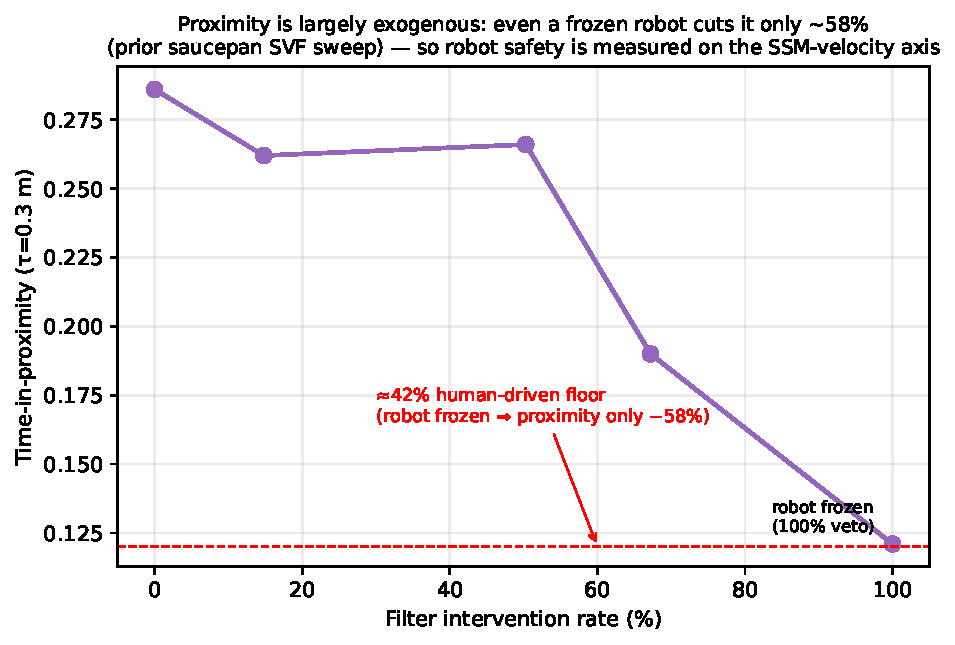
\includegraphics[width=0.62\textwidth]{fig4_exogenous_proximity}
\caption{The exogenous decomposition of proximity (the protocol's organising
measurement). Sweeping the runtime filter's intervention rate from
$0$ to $100\,\%$ (a fully frozen robot) removes only $\approx$58\,\%
of time-in-proximity; the residual $\approx$42\,\% is the coworker
approaching a stationary robot, a floor outside robot control.
Provenance: this sweep is the \emph{prior} saucepan SVF threshold
sweep, run before the intermittent-co-location experiments existed;
the two-axis protocol was fixed on its basis, not after seeing the
later results.}
\label{fig:exogenous-decomposition}
\end{figure}

\subsection{Axis Ownership}
\label{sec:setup:metrics:iso}

Proximity measures \emph{exposure}, but $\approx$42\,\% of it is
human-driven and no robot policy can remove it. We therefore retain
proximity as the exposure axis, it remains the natural axis for
\emph{policy-level} avoidance, whose anticipatory repositioning is
the one mechanism that can reduce how often co-location arises at
all, and use the velocity-adaptive \ssm{} margin
(\texttt{ep\_ssm\_violation\_actual\_rate},
Section~\ref{sec:bench:metrics:flavours}) as the robot-controllable
safety axis on which \emph{runtime filters} are judged: whether the
robot is moving slowly enough to stop before contact at the current
separation is a function of the robot's own commanded speed.
Every results table reports both axes for every configuration; the
conservative worst-case \texttt{ep\_ssm\_violation\_rate} appears
only in appendix tables (it saturates at $\sim$93\,\% on random
rollouts and carries little discriminative signal,
Section~\ref{sec:bench:metrics:flavours}).

\paragraph{Pre-registered decision rules.}
Three accept/reject rules were fixed before the corresponding sweeps
ran, and are reported with their outcomes: (i) the E1.1
observation-ablation bar, $\geq 20\,\%$ \ssm{}-rate reduction on at
least one (method, task) pair
(Section~\ref{sec:results:obs-bc}); (ii) the reactive-filter
gracefulness bar on the proximity axis, $\geq 30\,\%$ proximity
reduction at $\leq 25\,\%$ intervention
(Section~\ref{sec:results:reactive-taxonomy}); and (iii) the
boundary-condition rule for critic-gated scaling on
\texttt{saucepan\_to\_hob}, success $\geq 0.60$ \emph{and}
\ssm{}-actual $\leq 0.08$ for the gate to count as recovering
throughput (Section~\ref{sec:results:boundary}). Rule (iii)'s failure
on saucepan is itself a headline result, because it matches the
predicted boundary condition.

\subsection{Task Performance and the Safety Tax}
\label{sec:setup:metrics:task}

Two complementary task metrics so the \emph{cost of safety} on the
task is explicit:

\begin{itemize}[topsep=2pt,itemsep=1pt]
\item \texttt{success\_rate} (terminal task completion) is the
  primary task axis. \textbf{The $\Delta$~success column in the
  headline Table~\ref{tab:e4.1-feature-incremental} is the explicit
  ``did safety reduce task performance?'' answer}, computed as
  $(s_{\mathrm{row}} - s_{\mathrm{row\,1}})/s_{\mathrm{row\,1}}$
  with $s$ = success rate.
\item \texttt{steps\_to\_completion} (mean env-steps to terminal,
  among completed episodes) captures whether the policy preserves
  task completion but takes longer. A safe-and-slow policy and a
  safe-and-fast policy both register \texttt{success\_rate} = 1.0;
  \texttt{steps\_to\_completion} discriminates them. Under
  \iso{}~\ssm{}, the robot is expected to slow when the human
  approaches, so an increase here is expected behaviour rather than
  a failure mode, but it should be quantified.
\end{itemize}

\texttt{episode\_reward} (sum of $r^{\mathrm{task,shaped}}_t$ over
the episode) is reported in appendix tables as a tertiary axis
that combines task progress and the workspace-shaping signal.

\subsection{Tail Risk}
\label{sec:setup:metrics:tail}

Tail-risk metrics:
\begin{itemize}[topsep=2pt,itemsep=1pt]
\item $\cvar_{0.95}$ of \texttt{ep\_cost\_integral} (the tail metric
  matching the cost signal the policy was trained on).
\item $\cvar_{0.95}$ of \texttt{ep\_min\_separation} (a more
  human-readable tail metric).
\item 99\textsuperscript{th} percentile of
  \texttt{ep\_min\_separation}.
\end{itemize}
Each is computed over the union of 60 evaluation episodes per
configuration. Contact-force tail metrics are not reported because
of the open \pfl{} contact-detection limitation
(Section~\ref{sec:bench:cost}).

\subsection{Policy / Filter Interaction}
\label{sec:setup:metrics:interaction}

Three complementarity metrics for the runtime-mechanism question
(RQ2):
\begin{itemize}[topsep=2pt,itemsep=1pt]
\item \emph{Filter intervention rate}: fraction of env-steps where
  the runtime filter substitutes its fallback (zero-velocity for the
  veto, scaled velocity for speed-scaling). Reported in the headline
  Table~\ref{tab:e4.1-feature-incremental} and the taxonomy
  Table~\ref{tab:filter-taxonomy}; passthrough rate is its complement
  ($1 -$ intervention).
\item \emph{Internalisation curve}: filter intervention rate
  evaluated on intermediate snapshots of the Lagrangian-trained
  policy as training progresses. A \emph{falling} curve (rising
  passthrough) would be evidence the policy is learning the filter's
  job; E4.3 (Section~\ref{sec:results:interaction}) finds the opposite,
  a \emph{flat, elevated} curve, which is itself the diagnostic for the
  out-of-distribution veto.
\item \emph{Passthrough--task correlation}: at deployment, episodes
  with higher filter passthrough should also exhibit lower
  \texttt{steps\_to\_completion}, because every intervention swaps
  in the zero-velocity fallback and costs the policy a step or
  more of task progress. The harness records both per episode for
  the headline cells.
\end{itemize}

\section{Statistical Methodology}
\label{sec:setup:stats}

Every evaluation cell runs 20 episodes per evaluation seed across
three evaluation seeds (60 episodes), sampled from the relevant
\texttt{ParameterSpace}. Configurations involving a \emph{trained}
policy additionally pool three independently trained seeds, giving
180 episodes for the headline saucepan policy and composition rows
and for every row of the boundary-condition sweep; each table states
which applies. 95\,\% bootstrap confidence intervals (10{,}000
resamples over episodes) are reported for the headline safety
metric of each table. Directional claims are assessed by
bootstrap-CI overlap rather than parametric tests: episode-level
safety metrics are bounded, zero-inflated and heavily non-Gaussian,
so $t$-statistics would be poorly calibrated, whereas the CI
criterion is conservative and assumption-free. Two deliberate
exceptions to the three-trained-seed rule are flagged where they
occur: the intermittent-co-location Lagrangian budget sweep trains a
single seed per budget cell (six cells; the saucepan arm had already
established the seed-instability finding that would make per-cell
seed replication uninformative), and the WCSAC external reference is
a single seed per (task, budget) cell at 30 evaluation episodes,
reported with that caveat (Section~\ref{sec:results:wcsac}).

\label{sec:setup:smoke}%
Every script also carries a \texttt{--smoke} flag (a 5-minute CPU
validation); no multi-hour training was launched without passing the
relevant smoke gate first.

\section{Compute Budget}
\label{sec:setup:compute}

All training ran on single NVIDIA A100 (40\,GB) GPUs. The
persistent-co-location arc cost $\approx$220\,GPU-hours
(log-reconstructed), dominated by eighteen 40k-frame Lagrangian
fine-tunes at $\approx$9\,h each across the cost-form, budget, PID,
and fixed-$\lambda$ grids, plus the three-stage curriculum, the
confound control, the offline SVF pipeline, and snapshot evaluation.
The intermittent-co-location arc adds $\approx$230--280\,h, of which
the six 150k-frame from-scratch WCSAC runs dominate
($\approx$120--180\,h, estimated rather than log-reconstructed,
since they ran on a shared multi-GPU dispatcher). The project total
is roughly $450$--$500$\,GPU-hours; the carbon accounting
($\approx$40\,kg~CO\textsubscript{2}e under the 2024 UK grid
emissions factor) is derived in Appendix~\ref{app:sustainability}.


\section{The Unconstrained Baselines: Task-Competent, Not Compliant}
\label{sec:results:baseline}

The results below are organised by research question rather than by
phase; this section first establishes the unconstrained baseline
against which every later number is measured. The unconstrained
\cqnas{} policy at the end of stage~2 of the
curriculum (Section~\ref{sec:method:curriculum}) is task-competent
on \texttt{saucepan\_to\_hob}: under the headline \texttt{noisy}
perception condition it reaches \texttt{success\_rate} $= 0.85$.
The safety picture is poor (Table~\ref{tab:results:baseline}):
\texttt{ep\_proximity\_violation\_rate} $= 0.296$ ($\approx$30\,\% of steps within $\tau_{\mathrm{prox}} =
0.3$\,m) averaged across 60 eval episodes, the velocity-adaptive
\iso{}~\ssm{}-actual flag fires on $14.6\,\%$ of steps, and the mean
robot--human separation is only $0.132$\,m. The worst-case ISO bound
(conservative $S_p$ with $v_h = v_{h,\max}$) is saturated, firing on
$\sim$93\,\% of steps, which is why it is reported only for
traceability. Tail behaviour is dominated by the human's closest
lunge: $\cvar_{0.95}$ of \texttt{ep\_min\_separation} is
$\approx 0.005$\,m, with the single worst approach reaching
$\approx 0.002$\,m. The episode length is $\sim$449 control steps.

\begin{table}[htbp]
\centering
\caption{Baseline \iso{} compliance for the unconstrained
\cqnas{} policy on \texttt{saucepan\_to\_hob} under the
\texttt{coworker\_train} distribution (means $\pm$ 95\,\% bootstrap
CI, 3 seeds $\times$ 20 episodes). This is the ``before'' picture and
the floor against which every later result is measured: the policy is
task-competent yet violates proximity on a large fraction of
episodes, because nothing in its objective represents the human.}
\label{tab:results:baseline}
\small
\begin{tabular}{lcc}
\toprule
Metric & Unconstrained baseline & 95\,\% CI \\
\midrule
\texttt{success\_rate}                          & $0.85$  & $[0.75, 0.93]$ \\
\texttt{ep\_proximity\_violation\_rate}         & $0.296$ & $[0.23, 0.37]$ \\
\texttt{ep\_ssm\_violation\_actual\_rate}       & $0.146$ & $[0.10, 0.19]$ \\
\texttt{ep\_min\_separation} (mean, m)          & $0.132$ & -- \\
$\cvar_{0.95}$ \texttt{ep\_min\_separation} (m) & $\approx 0.005$ & -- \\
\bottomrule
\end{tabular}
\end{table}

\textbf{Reading.} The unconstrained baseline is the floor: a
task-competent policy that is \emph{not} \iso{} compliant under
sustained co-working. The deployment posture that \cqnas{}
ships with~\cite{seo2024cqnas} on \bigym{} would, under \sbigym{}'s
\coworker{} distribution, be within $0.3$\,m of the coworker on
$\approx$30\,\% of steps. Every reduction reported below is relative to
this floor.

\paragraph{Intermittent-co-location baselines.}
The same curriculum recipe yields competent unconstrained baselines
on the other two tasks (60 episodes each, \texttt{noisy},
\coworker{}): \texttt{dishwasher\_close} reaches $0.77$ success with
\ssm{}-actual $0.176$ and proximity $0.246$;
\texttt{drawers\_open\_all} reaches $0.82$ success with \ssm{}-actual
$0.100$ and proximity $0.211$. The drawers policy is naturally slower
(mean robot velocity $0.19$ vs.\ dishwasher's $0.44$\,m/s), which is
why its baseline \ssm{}-violation rate is half the dishwasher's, a
fact that later bounds how much a velocity-axis filter can add there
(Section~\ref{sec:results:r2-gated}).


% =============================================================================
% PART IV-B: RESULTS
% =============================================================================

% =============================================================================
\chapter{Results: Two Regimes, One Law}
\label{ch:eval}
% =============================================================================

\section{The Shape of the Evidence}
\label{sec:results:ablation-map}

This chapter reports the evaluation in three movements. The first
(Section~\ref{sec:results:r1}) takes the persistent-co-location
task, \texttt{saucepan\_to\_hob}, from the unconstrained baseline
through every safety mechanism to the division of labour that works
there. The second (Section~\ref{sec:results:r2}) repeats the
exercise on the two intermittent-co-location tasks, where the
verdicts reverse. The two movements will appear to contradict each
other, and the third (Section~\ref{sec:results:boundary}) shows that
they are one finding: the chapter closes by transplanting the
intermittent-regime winner onto the persistent task under a decision
rule fixed in advance, with the regime map predicting, correctly,
that it must fail there.

The evaluation is deliberately ablation-led: each major component is
removed, replaced, or retuned to test whether it actually
contributes. Observation without a safety gradient does not produce
safety (Section~\ref{sec:results:obs-bc}). The cost budget, not the
cost form, decides whether the constraint binds, and PID auto-tuning
is seed-unstable at the feasibility boundary
(Section~\ref{sec:results:budget}). The runtime override form is
decisive, in that a binary veto breaks chunked-policy coherence where
graded scaling preserves it
(Sections~\ref{sec:results:reactive-taxonomy}
and~\ref{sec:results:r2-veto}), and the gate-design ablations show
the gate threshold to be the dominant dial
(Section~\ref{sec:results:r2-ablations}). Each retained component of
the final architecture survives a specific failure mode of a simpler
alternative.

\section{Persistent Co-location: Safety Must Be Trained In}
\label{sec:results:r1}

This section is the persistent-co-location arm of the regime map. On
\texttt{saucepan\_to\_hob} the coworker occupies the robot's working
volume nearly continuously: a separation-triggered filter would be
active on $\approx$44--62\,\% of steps (measured directly in
Section~\ref{sec:results:boundary}). The claim this section
establishes is the first half of the regime map: \emph{where
co-location is persistent, no runtime mechanism reduces exposure
gracefully, and a fixed-multiplier constrained policy does, cutting
proximity violations by $23\,\%$ at $0.76$ success, reproducibly
across seeds}. The evidence runs in order: observation alone is not
a safety mechanism; what it takes to make the constraint bind; what
reactive filtering can and cannot contribute on each axis; the
headline comparison and the composition's ceiling; and how far the
result stretches under perception noise, a held-out coworker, and
the worst-case tail.

\subsection{Observation Alone Is Not a Safety Mechanism}
\label{sec:results:obs-bc}

Before any constraint was trained, a behaviour-cloning pilot (E1.1:
ACT, four tasks, observation modes
\texttt{off}/\texttt{oracle}/\texttt{noisy}, no violation penalty)
tested whether merely \emph{seeing} the human improves safety,
against a criterion fixed in advance: a $\geq 20\,\%$
\ssm{}-violation reduction. No cell cleared the bar. The best case
(\texttt{drawers\_open\_all}) improved by $13.7\,\%$, and on three of
four tasks the oracle channel made violations \emph{worse}, most
sharply on \texttt{saucepan\_to\_hob} ($0.135 \to 0.203$) even as it
raised task success ($0.22 \to 0.58$). The policy uses human state
to route around obstructions and complete the task, not to keep
distance, because nothing in its objective rewards the latter.
Observation without a safety gradient is at best inert and at worst
counterproductive, which is what motivates training the constraint
into the policy. (Behaviour cloning alone cannot distinguish
``channel useless'' from ``cloning marginalises a channel
uncorrelated with demonstrated actions''. The perception sweep of
Section~\ref{sec:results:obs-rl} resolves the ambiguity under
non-degenerate constrained training.)

\subsection{The Cost Budget, Not the Cost Form, Is the Operative Variable}
\label{sec:results:cost-signal}
\label{sec:results:budget}

Two ablations locate what makes the constraint bind. The first
(E3.1) ablated the \emph{form} of the per-step cost $c_t$, holding
the rest of the agent fixed: a continuous graded signal
($c_t = \min(1,\max(c^{\ssm},c^{\pfl})) \in [0,1]$,
Equation~\ref{eq:c-total}) against a binary worst-case indicator, at
the nominal tight budget $d = 0.01$. The comparison is degenerate:
both forms collapse to $0\,\%$ task success (at deployment proximity
$0.013$ and $0.024$ respectively). The cause is feasibility, not
form. The dual variable, updated as
$\lambda \leftarrow \lambda + k\,(\bar c - d)$, can stabilise only
if some policy achieves average cost $\bar c \le d$, and no policy
can: $\approx$42\,\% of the baseline's $0.296$ proximity is
exogenous (Section~\ref{sec:exogenous}), so the achievable cost
floor is $\approx 0.42 \times 0.296 \approx 0.12$, an order of
magnitude above the budget. The multiplier winds up regardless of
the cost signal's shape, the $-\lambda Q_c$ term swamps the reward
objective, and the policy abandons the task to minimise cost. (A
fixed reward penalty with no dual variable sidesteps the windup, but
its apparent training-time reduction did not survive
deployment-faithful evaluation, so it is not adopted either.)

The second ablation (E3.2) sweeps the variable that \emph{is}
operative, the budget $d$. The sweep does not trace a smooth
safety/throughput Pareto. It exposes a sharp feasibility boundary:
every budget at or below the task's inherent per-step cost collapses
task success, with continuous-cost runs at
$d \in \{0.001, 0.05, 0.1\}$ reaching success $0.00$, $0.00$, $0.13$
respectively, all essentially task-abandoning. The single budget
that is both feasible and non-trivial, $d = 0.3$ at the task's
inherent cost, does not give a stable operating point under PID
auto-tuning: it sits \emph{on} the feasibility boundary, so the dual
variable is decided by each seed's stochastic cost trajectory.
Figure~\ref{fig:lambda-regimes} shows the three seeds at $d = 0.3$
converging to $\lambda = 0.000, 0.267, 3.855$, producing an
unconstrained policy, a graceful avoidance basin, and a windup
collapse to zero success. The graceful regime reproduces in only one
of three seeds. This is why the headline policy
(Section~\ref{sec:results:headline-feature-table}) pins $\lambda$ at
a fixed value rather than auto-tuning it: the budget loop is
ill-conditioned exactly where the only feasible budget lies.

\begin{figure}[htbp]
\centering
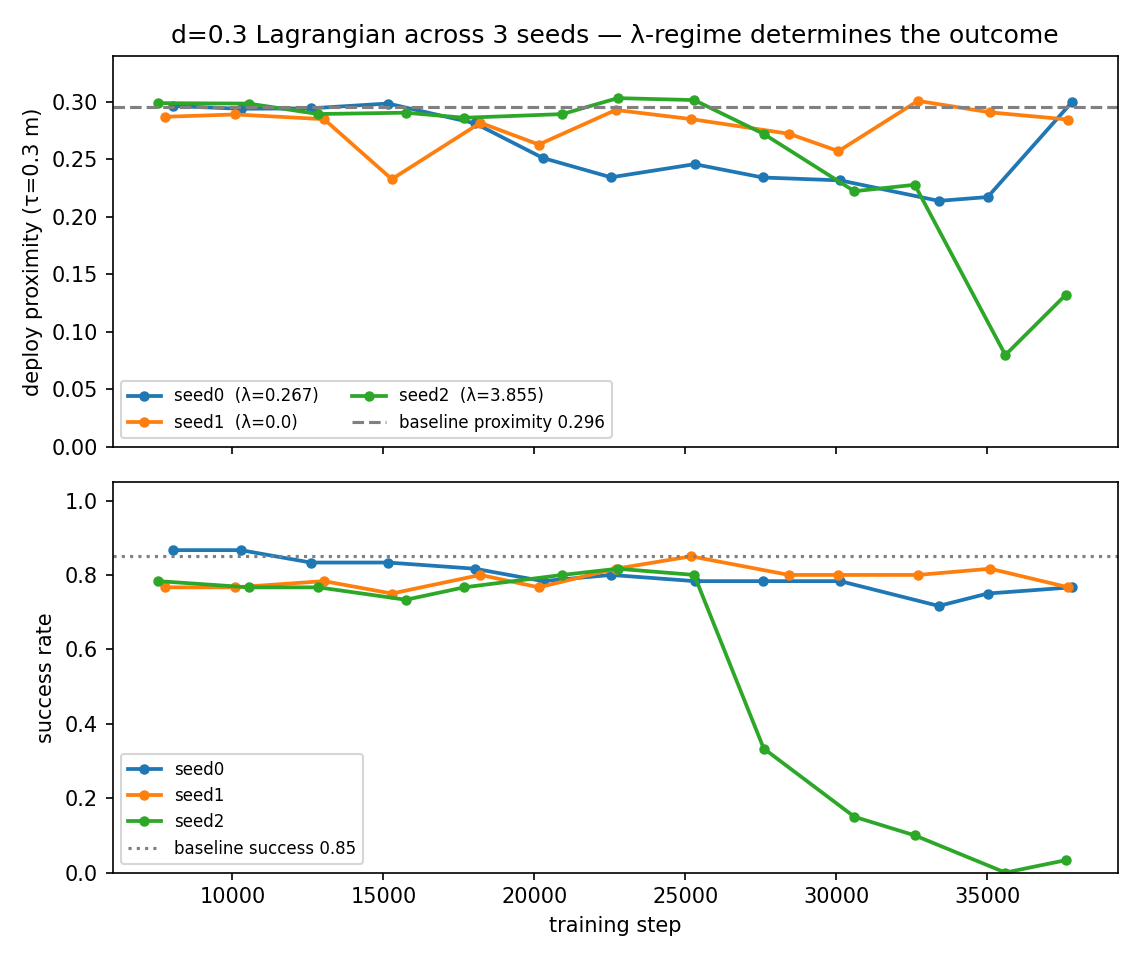
\includegraphics[width=0.55\textwidth]{d0p3_3seed_lambda_regimes.png}
\caption{The budget-feasibility experiment (E3.2; RQ1).
PID-Lagrangian at the only feasible
budget $d = 0.3$, three seeds. Top: deployment proximity-violation
rate ($\tau = 0.3$\,m) versus training step; bottom: task success. The
seeds converge to $\lambda = 0.000$ (seed~1, unconstrained, flat at
the baseline $\approx$0.30), $\lambda = 0.267$ (seed~0, a graceful
sub-0.26 avoidance basin), and $\lambda = 3.855$ (seed~2, windup
collapse, success $\to 0$). Because $d = 0.3$ coincides with the
task's inherent cost, the dual variable carries too little signal to
auto-tune stably, motivating the fixed-$\lambda$ headline.}
\label{fig:lambda-regimes}
\end{figure}

\subsection{The Reactive-Filter Pareto Frontier}
\label{sec:results:filter-pareto}

The offline SVF was trained at $\alpha_{\mathrm{CQL}} = 5.0$ and
swept over the veto threshold $R$ on a held-out validation set (three
seeds, 20 episodes each). With the filter disabled ($R = 0$) the
swept \texttt{ep\_proximity\_violation\_rate} is $0.286$, which
matches the unconstrained benchmark baseline of $0.296$ to within
sampling error; this agreement is the validation check that the
sweep environment reproduces the deployment environment.

The sweep does \emph{not} expose an operating point that reduces
geometric proximity cheaply: $R = 2.25$ cuts proximity by only
$\approx$8\,\% at $\approx$15\,\% intervention, a one-third
reduction needs $\approx$67\,\% intervention, and even vetoing
\emph{every} step caps the reduction at $\approx$58\,\%, the
decomposition of Section~\ref{sec:exogenous} seen from the filter
side. We therefore pin the operating point at the light backstop
$R = 2.25$ and read the veto as an \iso{}~\ssm{} velocity backstop,
not a proximity reducer; proactive proximity reduction is delegated
to the constrained policy
(Section~\ref{sec:results:headline-feature-table}).

\paragraph{The reactive-fallback dilemma.}
A natural objection is that a more aggressive fallback would let the
filter reduce proximity directly. A fallback sweep on the
unconstrained baseline at matched intervention rates rules this out.
Zero-velocity braking holds station: it trims mean robot speed (the
velocity-backstop effect) but leaves proximity unchanged
($0.296 \to 0.303$), because the robot simply dwells while the human
approaches. An aggressive retreat cuts proximity sharply
($0.296 \to 0.095$) but only by having the robot flee: success
collapses from $0.85$ to $0.18$, mean speed rises sixfold
($0.29 \to 1.70$\,m/s), and the \ssm{}-actual rate \emph{worsens}
($0.147 \to 0.180$) because a fast-retreating robot is itself an
\ssm{} hazard. A gentle retreat does neither job. No reactive
setting buys geometric separation at acceptable success and speed:
against an approaching human, reducing proximity requires sustained,
anticipatory robot motion, which a one-step reactive filter cannot
supply. The veto remains independently useful as a deployment
backstop that trims mean speed without any retraining, but the
graded margin \iso{} prescribes needs the speed-scaling filter
(Section~\ref{sec:results:reactive-taxonomy}). This is the empirical
case for assigning the exposure axis to the policy arm, revisited in
Section~\ref{sec:disc:filter-role}.

\subsection{The Headline Comparison: A Division of Labour}
\label{sec:results:headline-feature-table}

\textbf{Main comparison.} The central question of the
architecture is which mechanism reduces which \iso{} axis, and how the
mechanisms compose. The answer is a \emph{division of labour}: the
proactive constrained-RL policy owns the geometric-proximity axis and a
complementary-axis runtime filter owns the velocity (\ssm{}-actual)
axis. Table~\ref{tab:e4.1-feature-incremental} reports the four
configurations that establish this; the two reactive-veto
configurations the architecture was originally built around are
covered in Section~\ref{sec:results:reactive-taxonomy}, and the
both-axis composition is analysed in
Section~\ref{sec:results:joint-coverage}.

\paragraph{The proactive policy reduces proximity, reproducibly.}
The fixed-$\lambda$ ($\lambda = 0.1$) Lagrangian policy reduces
\texttt{ep\_proximity\_violation\_rate} from the baseline $0.296$ to
$0.228$, a $22.8\,\%$ reduction (bootstrap 95\,\% CI $[0.194, 0.264]$),
at $0.76$ task success (CI $[0.70, 0.82]$), pooled over three seeds
(180 episodes). Each
seed's selected operating point is below the baseline; the
velocity-adaptive \ssm{}-actual rate also improves
($0.146 \rightarrow 0.112$, $-23\,\%$) and mean robot velocity rises
only $\sim$8\,\%. This is the graceful proximity reduction the reactive
filter could not achieve (Section~\ref{sec:results:filter-pareto}).
The magnitude is bounded by the $\approx$42\,\% exogenous floor
(Section~\ref{sec:exogenous}): it captures roughly $40\,\%$ of the
\emph{reducible} (robot-driven) proximity. Modest in absolute terms,
but the reactive filter captured essentially none of it at acceptable
cost.

\begin{table}[htbp]
\centering
\caption{Experiment E4.1 (\textbf{the headline}). The division of
labour between the proactive policy and a complementary-axis runtime
filter on \texttt{saucepan\_to\_hob} under \texttt{coworker\_train},
\texttt{noisy} perception. Rows 1 and 3 evaluate the single stage-2
baseline policy over 60 episodes (3 evaluation seeds $\times$ 20);
rows 2 and 4 pool three independently trained seeds (180 episodes).
Brackets are 95\,\% bootstrap CIs. The policy owns the
geometric-proximity axis ($\tau = 0.3$\,m); the graded speed-scaling
filter owns the velocity-adaptive \ssm{}-actual axis; only their
composition reduces both at once, at a multiplicative success cost.
$\Delta$ columns are relative to the unconstrained baseline (negative
is safer). The two SVF-veto configurations are in
Table~\ref{tab:filter-taxonomy}.}
\label{tab:e4.1-feature-incremental}
\small
\setlength{\tabcolsep}{4pt}
\resizebox{\textwidth}{!}{%
\begin{tabular}{lcccccc}
\toprule
Configuration & \texttt{succ.} & \texttt{prox.viol} & $\Delta$ prox.\ & \texttt{ssm-act.} & $\Delta$ ssm.\ & Interv.\ \\
\midrule
Unconstrained baseline                 & $0.85$ & $0.296\,[0.23, 0.37]$ & --       & $0.146\,[0.10, 0.19]$ & --       & -- \\
Proactive policy ($\lambda{=}0.1$)     & $0.76$ & $\mathbf{0.228}\,[0.19, 0.26]$ & $\mathbf{-23\,\%}$ & $0.112\,[0.09, 0.13]$ & $-23\,\%$ & -- \\
Speed-scaling filter (on baseline)     & $0.53$ & $0.273\,[0.21, 0.35]$ & $-8\,\%$ & $\mathbf{0.048}\,[0.03, 0.07]$ & $\mathbf{-67\,\%}$ & $45\,\%$ \\
\textbf{Policy $+$ speed-scaling (composition)} & $\mathbf{0.44}$ & $0.250\,[0.21, 0.29]$ & $-15\,\%$ & $0.065\,[0.05, 0.08]$ & $-55\,\%$ & $40\,\%$ \\
\bottomrule
\end{tabular}%
}
\end{table}

\paragraph{Operating-point selection must be safety-aware.}
A methodological point underwrites the policy row. At the feasible
budget the avoidance does not live at the peak-success checkpoint:
\texttt{snapshot\_best} (peak success) and the final checkpoint both
deploy at $\approx$baseline proximity ($\approx$0.30), because
selecting on task success picks \emph{against} the cost constraint. The
avoidance lives in a mid-training basin ($\sim$20k--35k steps, several
consecutive checkpoints at $0.21$--$0.25$ with success $0.72$--$0.80$
and \ssm{}-actual improved). The operating point must therefore be
chosen by a \emph{safety-aware} rule (lowest deployment proximity at a
success floor), not by peak success; selecting on success produced two
false-null results before the basin was found. Each seed's selected
basin checkpoint is shown in Figure~\ref{fig:fixlam}; that the basin
appears consistently across all three seeds under fixed $\lambda$ is
what makes the reduction reproducible, in contrast to the PID
instability of Figure~\ref{fig:lambda-regimes}.

\paragraph{The basin is constraint-driven, not selection noise.}
Selecting a checkpoint by a deployment metric invites the objection
that the ``basin'' is evaluation noise harvested by the rule. Four
observations rule this out: the $\lambda = 0$ seed, processed by the
\emph{same} rule, shows no basin (flat at $\approx$0.30 with
isolated dips); the basin is a \emph{run} of consecutive checkpoints
at $0.21$--$0.26$ proximity with success $0.72$--$0.80$
(Figure~\ref{fig:fixlam}), not a single dip; \ssm{}-actual
co-improves inside it, which uncorrelated proximity noise would not
produce; and the selected point also sits below the
\emph{no-shaping} baseline at matched success (the $-12\,\%$
comparison below). When $\lambda$ engages, the constraint does work;
when it is slack, no selection rule manufactures a basin.

\begin{figure}[htbp]
\centering
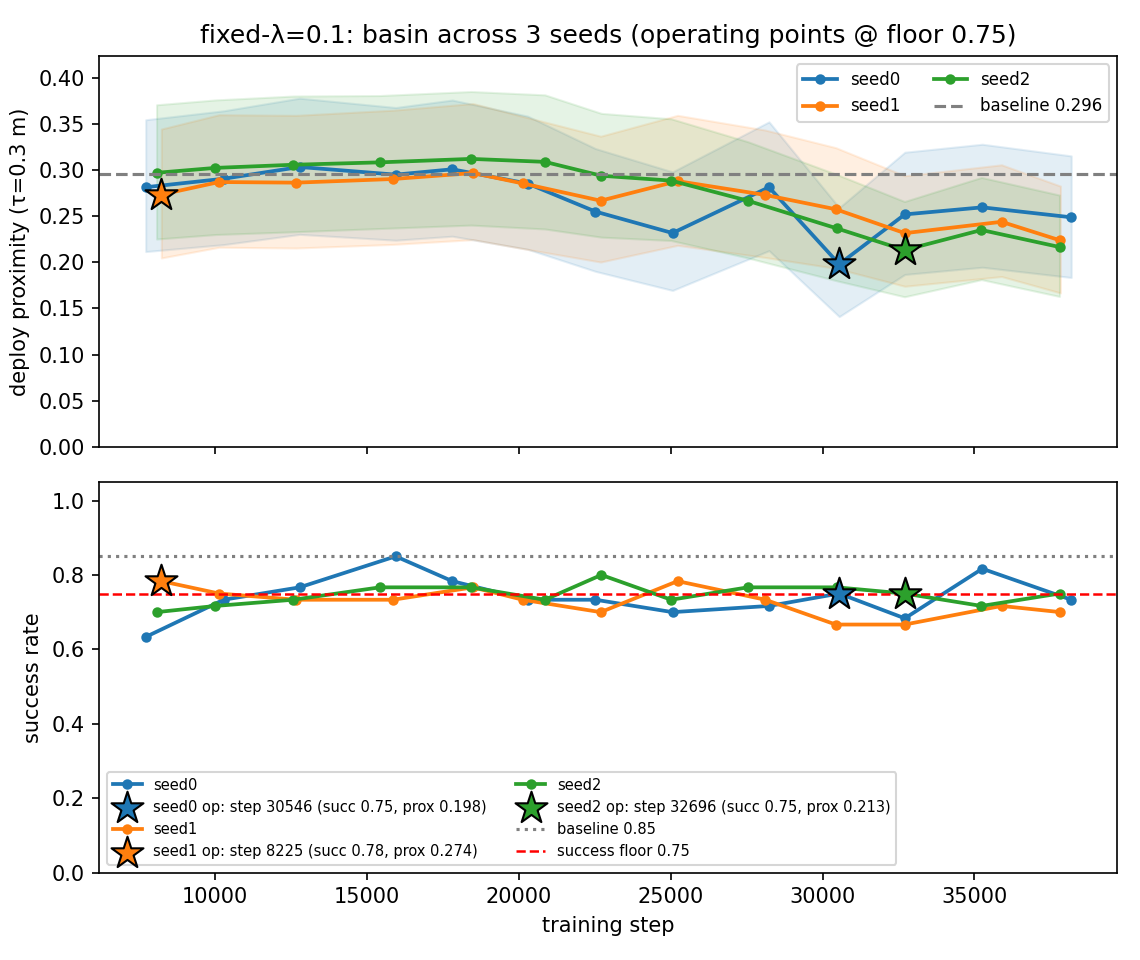
\includegraphics[width=0.55\textwidth]{fixlam0p1_3seed_floor075.png}
\caption{The fixed-$\lambda = 0.1$ policy across three seeds (stars
mark the safety-aware operating point at a success floor of $0.75$).
Top: deployment proximity-violation rate; bottom: success. Unlike the
PID runs (Figure~\ref{fig:lambda-regimes}), all three seeds behave
consistently and each reaches a sub-baseline proximity basin in
mid-training, giving the pooled $0.228$ at $0.76$ success. Fixing
$\lambda$ removes the ill-conditioned budget loop that made the PID
controller seed-unstable.}
\label{fig:fixlam}
\end{figure}

\paragraph{Controlling for the workspace-shaping confound.}
The unconstrained baseline carries a mild workspace-distance reward
($\beta = 0.05$, Section~\ref{sec:bench:workspace}) that anchors the
end-effector in the task workspace. A natural objection is that this
inflates the baseline's proximity and hence the policy's apparent
reduction. Ablating it: the no-shaping baseline is $0.75$ success /
$0.258$ proximity, versus the shaping baseline's $0.85$ / $0.296$. So
shaping is a \emph{task-success aid that incidentally raises
proximity} (it keeps the robot where the coworker reaches), not a
safety term. Crucially, the Lagrangian policy ($0.228$ at $0.76$) sits
below the no-shaping baseline too, a $-12\,\%$ proximity reduction at
matched success, so the headline $-23\,\%$ (against the matched-recipe
baseline) is not an artefact of an inflated reference. We report both:
$-23\,\%$ (isolated constraint effect, shaping held fixed) and
$-12\,\%$ (confound-controlled, against the vanilla baseline).

\paragraph{The velocity axis is the filter's, and only a graded filter
reaches it.}
A runtime filter's canonical \iso{} role is the velocity axis. The
graded speed-scaling filter delivers it: on the baseline it drives
\ssm{}-actual from $0.146$ to $0.048$ ($-67\,\%$) at its optimum
($d_{\mathrm{slow}} = 0.40$\,m), with proximity essentially unchanged
($0.296 \rightarrow 0.273$). It is the only filter in the taxonomy
that meaningfully reduces \emph{any} \iso{} axis on its own terms;
the binary veto, despite also slowing the robot, leaves
\ssm{}-actual at $0.148 \approx$ baseline, a stop-or-go veto does not
maintain the graded margin the standard prescribes. The success
cost, however, is not an artefact of the $0.40$\,m setting: even the
gentlest swept point ($d_{\mathrm{slow}} = 0.25$\,m) intervenes on
$37\,\%$ of steps, co-location is persistent, so some part of the
robot is nearly always inside the slow radius, and still costs a
third of task success at \emph{less} velocity-axis gain. The
reactive cost is paid at every operating point; only its exchange
rate moves.

\paragraph{The composition is the only both-axis-compliant
configuration, and it costs success.}
Composing the policy with the speed-scaling filter is the \emph{only}
configuration that reduces both \iso{} axes at once: geometric
proximity $0.250$ (retained from the policy's $0.228$, CIs overlap)
\emph{and} \ssm{}-actual $0.065$ ($-42\,\%$ against the policy's
$0.112$, the filter's contribution). Each component alone leaves the
\emph{other} axis near baseline (policy: \ssm{}-actual $0.112$;
filter-alone: proximity $0.273 \approx$ baseline). The cost is task
success: $0.85 \rightarrow 0.44$. The proactive cost ($0.85 \to 0.76$,
$\times 0.89$) and the reactive cost ($\times 0.58$) stack
\emph{multiplicatively}, and the composition beats neither specialist
on that specialist's own axis (the policy still wins proximity
$0.228 < 0.250$; the filter still wins velocity $0.048 < 0.065$). The
composition is the joint-coverage compromise, not a per-axis champion.
Both measured safety axes are improved in this regime only by composing
the proactive policy with a complementary runtime filter, and that
composition makes the safety--throughput trade explicit, with a cost
dial tunable through $\lambda$ and $d_{\mathrm{slow}}$
(Section~\ref{sec:results:joint-coverage}).

\paragraph{Sim-to-real perception.}
The whole table is evaluated under \texttt{bodyslam=noisy}, the
realistic deployment condition and the filter's native distribution
(Section~\ref{sec:setup:perception-mode}). The policy's reduction
survives this noisy, lagged perception unchanged (E3.6,
Section~\ref{sec:results:obs-rl}): the architecture claim is reported
under deployment-relevant perception, not only under oracle state.

\subsection{The Reactive-Filter Taxonomy: Freeze versus Flee}
\label{sec:results:reactive-taxonomy}

The headline filter is the graded speed-scaling one. The architecture
was, however, originally built around a learned \textsc{CQL} safety
value function used as a veto, and the journey from that design to the
graded filter is itself a result. We evaluated every reactive modality
available, learned and model-based, and none reaches the proactive
policy's graceful operating point. The reason is structural: a reactive
filter acts only \emph{once the human is already close}, when the only
moves are to \emph{freeze} (and dwell in the danger zone) or to
\emph{flee} (and abandon the task). Table~\ref{tab:filter-taxonomy}
summarises the taxonomy. The claim is
scoped deliberately: \emph{no reactive filter gracefully reduces
proximity under persistent co-location}. It is a statement about the
exposure axis in this regime, not about reactive filtering in
general; Section~\ref{sec:results:r2} shows what reactive mechanisms
\emph{can} deliver, on the velocity axis, where co-location is
intermittent and genuinely-safe windows exist.

\begin{table}[htbp]
\centering
\caption{The reactive-filter taxonomy on \texttt{saucepan\_to\_hob}
(\coworker{}, \texttt{noisy}); every row is 60 evaluation episodes,
and rows involving the constrained policy use the seed-0 trained
policy (the pooled three-trained-seed policy numbers are in
Table~\ref{tab:e4.1-feature-incremental}). Every reactive modality,
learned or model-based, is bounded by the freeze-versus-flee dilemma:
it either freezes (and proximity does not fall) or flees (and task
success collapses). None reaches the proactive policy's frontier
(success $0.75$, proximity $0.198$ at seed~0; $0.76$/$0.228$ pooled).
The SVF veto applied to the \emph{policy} (the architecture's
original composition design) is worse than the policy alone.}
\label{tab:filter-taxonomy}
\small
\begin{tabular}{llccc}
\toprule
Filter & Mechanism & Proximity & Success & Interv.\ \\
\midrule
Learned veto (SVF), on baseline   & velocity backstop (freeze) & $0.303$ & $0.78$ & $15\,\%$ \\
Learned veto (SVF), on policy     & freeze $\to$ dwell         & $0.265$ & $0.62$ & $48\,\%$ \\
Model-based base-dodge (CBF)      & flee (retreat base)        & $0.150$ & $0.57$ & $1.3\,\%$ \\
Model-based EE-retract (CBF)      & flee (retract arm)         & $0.155$ & $0.50$ & $5.8\,\%$ \\
\textbf{Proactive policy ($\lambda{=}0.1$)} & \textbf{anticipatory avoid} & $\mathbf{0.198}$ & $\mathbf{0.75}$ & -- \\
\bottomrule
\end{tabular}
\end{table}

\paragraph{The learned veto freezes.}
On the baseline, the SVF veto with a zero-velocity fallback
($R = 2.25$, $15\,\%$ intervention) does not reduce geometric proximity
($0.296 \rightarrow 0.303$, within noise); it only trims mean robot
velocity ($-8\,\%$), acting as an \ssm{} \emph{velocity backstop}
(Section~\ref{sec:results:filter-pareto}). Applied on top of the
already-avoiding policy, it is \emph{counterproductive}: proximity
worsens ($0.198 \rightarrow 0.265$) and success falls
($0.75 \rightarrow 0.62$), at a $48\,\%$ intervention rate (versus
$15\,\%$ on the baseline). The mechanism is distribution shift: the SVF
critic was collected on \emph{baseline} rollouts, so it is out of
distribution on the avoiding policy and over-vetoes, and each veto
zeroes robot velocity, re-introducing the freeze/dwell failure. A
threshold sweep confirms this is not mis-thresholding, $R \in [1.0,
2.25]$ gives $39$--$48\,\%$ intervention and proximity $0.27$--$0.28$ at
every setting, and re-collecting the critic on the policy's own
rollouts (on-policy) still yields no graceful operating point: at
$\le 25\,\%$ intervention every threshold \emph{increases} proximity,
and proximity falls only at $65$--$100\,\%$ intervention where the robot
is essentially frozen. Neither critic meets the pre-registered
gracefulness bar ($\geq 30\,\%$ proximity reduction at $\leq 25\,\%$
intervention, Section~\ref{sec:setup:metrics}). Both the
baseline-trained and on-policy critics fail at every threshold, so the
limit is the reactive paradigm, not the critic's calibration.

\paragraph{The model-based filter flees.}
A geometric control-barrier-style ``directional-dodge'' filter (no
learned critic) \emph{does} reduce proximity where the veto cannot,
$0.198 \rightarrow 0.150$ at $d_{\mathrm{target}} = 0.35$\,m and only
$1.3\,\%$ intervention, but by \emph{fleeing}: the base retreats,
episodes stretch from $\sim$450 to $620$--$770$ steps, and success
falls to $0.57/0.43/0.35$ as $d_{\mathrm{target}} = 0.35/0.45/0.55$,
with proximity flooring at $\approx$0.14 regardless (the exogenous
floor). There is no harmless-backstop setting: even at the minimal
$d_{\mathrm{target}} = 0.30$\,m ($1.1\,\%$ intervention) success
falls $0.75 \rightarrow 0.58$, because even rare dodges land at
task-critical moments. The same flee appears whichever part of the
robot dodges: retracting the \emph{end-effector} (an arm ``flinch''
via a damped-Jacobian step) is worse in the useful regime ($0.50$
success at $d = 0.35$; the EE is the closest pair, so it intervenes
far more often, and retracting the arm \emph{is} pausing the task).
The flee is structural: the task and the hazard are co-located, so a
separation barrier is satisfiable only by radial retreat, which is
retreat from the workspace. Eliminating the flee requires
anticipation, which is exactly what the constrained policy provides;
``fixing'' the flee inside a reactive filter amounts to reinventing
the policy.

\subsection{Joint ISO Coverage: The Composition and Its Ceiling}
\label{sec:results:joint-coverage}

The two preceding subsections separate cleanly onto the two \iso{}
axes (Figure~\ref{fig:axis-division}).
Figure~\ref{fig:velocity-axis} makes the velocity axis explicit:
on \ssm{}-actual the speed-scaling filter is the specialist
($\rightarrow 0.048$), the policy also helps via avoidance
($\rightarrow 0.112$) because keeping further from the human lowers the
required margin, and the SVF veto does not help at all ($0.148 \approx$
baseline). Figure~\ref{fig:joint-coverage} then plots both axes
together: only the policy-plus-speed-scaling composition reaches the
both-safe corner (low proximity \emph{and} low \ssm{}-actual), and it
is strictly better than the SVF-veto composition, which \emph{degraded}
proximity with no velocity gain. A complementary-axis, model-based
filter composes additively where a redundant-axis, out-of-distribution
\emph{learned} filter destroyed.

The composition's success cost ($0.85 \to 0.44$, analysed in
Section~\ref{sec:results:headline-feature-table}) should be read as
\emph{the persistent-co-location regime's ceiling}, not as a defect of
the composition: when the coworker is co-located most of the time,
any separation-triggered speed response is active most of the time
(measured directly in Section~\ref{sec:results:boundary}), so the
reactive cost is paid almost everywhere and stacks with the
proactive cost. Under this regime, both-axis \iso{} safety is
purchasable only at stacked cost; whether a smarter trigger
(a learned critic gating the scaler) can avoid that cost is exactly
the question the intermittent-co-location chapter answers in the
affirmative, and Section~\ref{sec:results:boundary} answers in the
negative \emph{for this regime}.

\begin{figure}[htbp]
\centering
\begin{subfigure}[t]{0.48\textwidth}
  \centering
  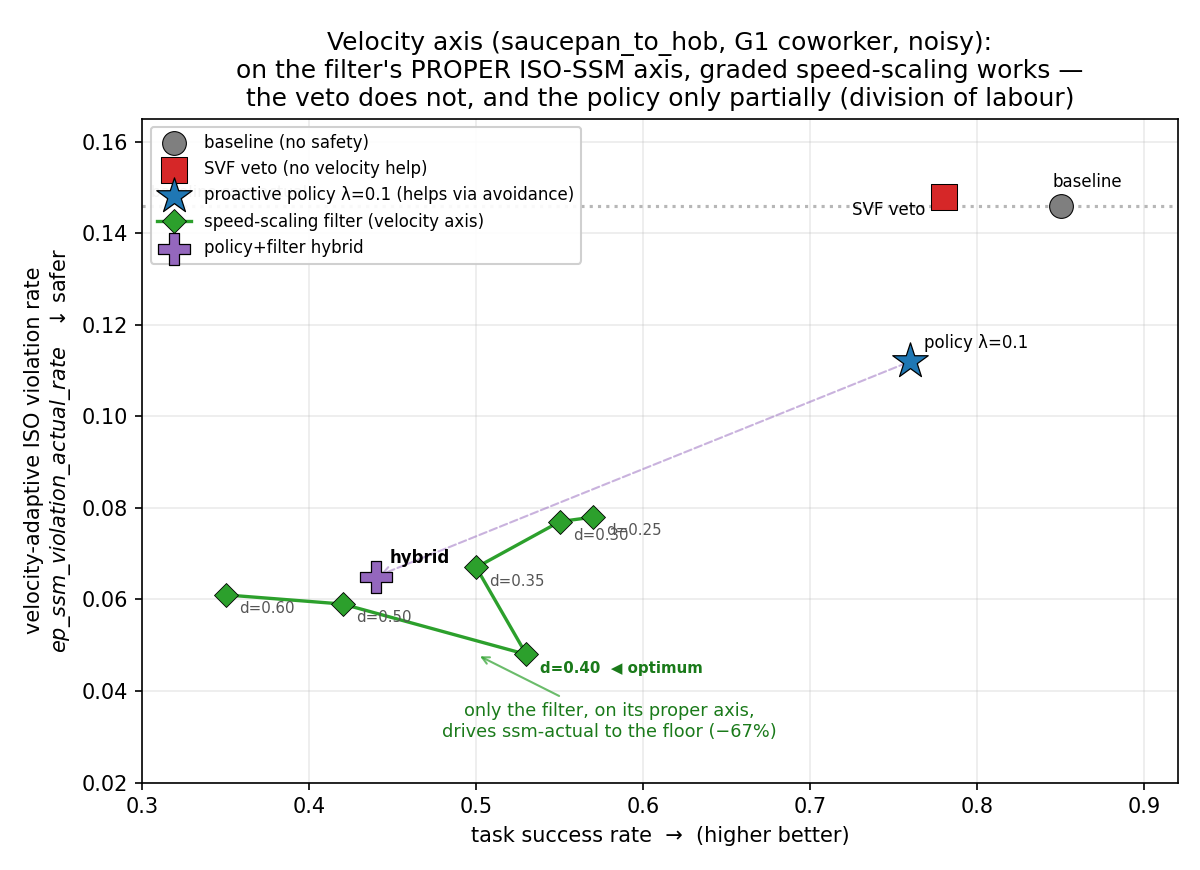
\includegraphics[width=\linewidth]{velocity_axis.png}
  \caption{The velocity (\ssm{}-actual) axis: the graded
  speed-scaling filter is the specialist; the policy also reduces it
  via avoidance; the veto does not maintain the graded margin and
  leaves it at baseline.}
  \label{fig:velocity-axis}
\end{subfigure}\hfill
\begin{subfigure}[t]{0.48\textwidth}
  \centering
  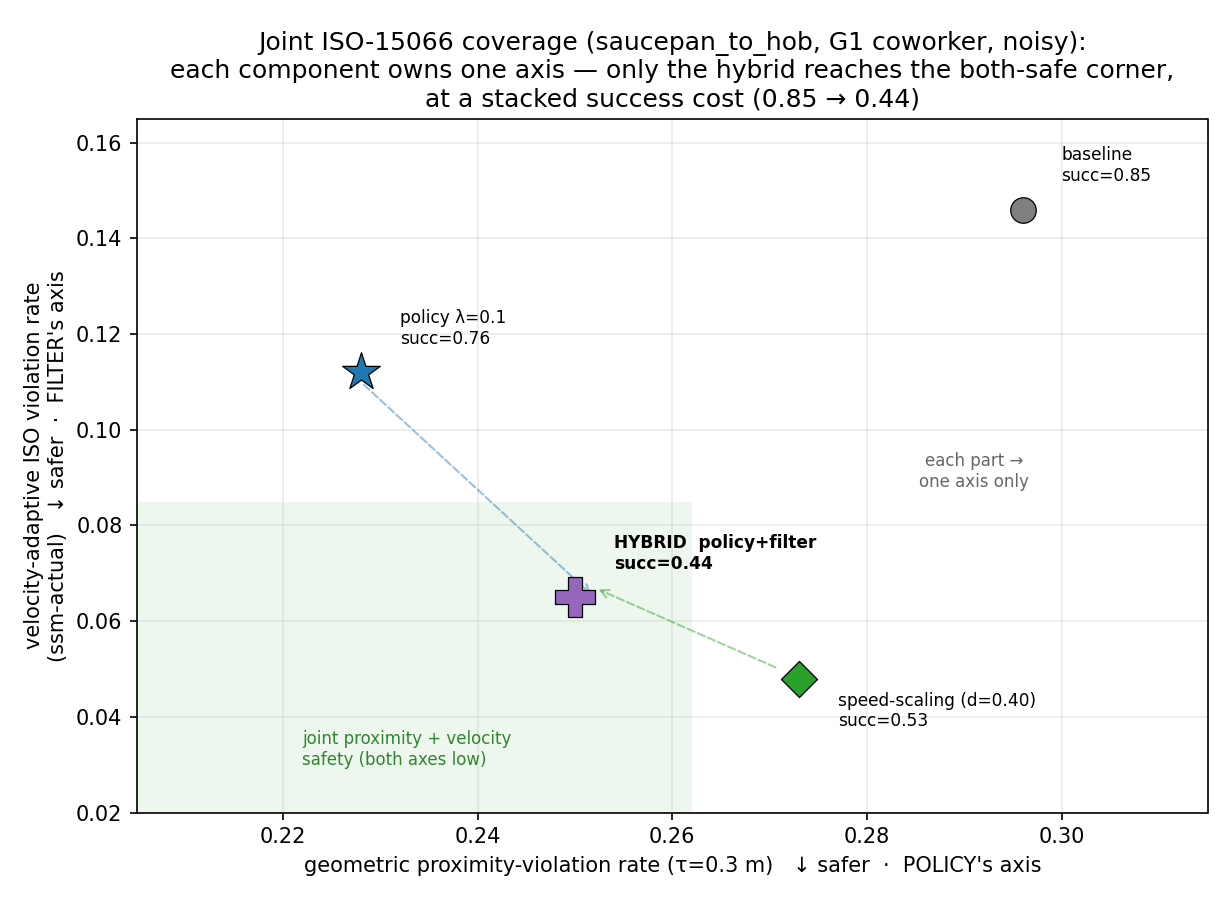
\includegraphics[width=\linewidth]{joint_coverage.png}
  \caption{Joint coverage: proximity ($x$, policy's axis) vs.\
  \ssm{}-actual ($y$, filter's axis). Only the composition reaches
  the both-safe corner, at success $0.44$; it beats neither
  specialist on that specialist's own axis.}
  \label{fig:joint-coverage}
\end{subfigure}
\caption{The two-axis division of labour on
\texttt{saucepan\_to\_hob} (60-episode cells, \texttt{noisy}
perception, \coworker{} distribution) and what composing the
specialists buys. The policy owns the proximity axis, the graded
speed-scaling filter owns the velocity axis, and only their
composition reaches the corner where both \iso{} axes improve at
once, at a success cost ($0.85 \to 0.44$) that
Section~\ref{sec:results:boundary} shows to be the persistent
regime's ceiling rather than a tuning defect.}
\label{fig:axis-division}
\end{figure}

\subsection{The Policy Does Not Internalise the Filter}
\label{sec:results:interaction}

If the policy and the SVF veto were complementary in the originally
hypothesised sense, the filter's required intervention rate would
\emph{fall} as the Lagrangian policy is trained, the policy
progressively taking over the filter's job. E4.3 evaluates the SVF
veto's intervention rate on intermediate snapshots of the
fixed-$\lambda$ policy across training. It does \emph{not} fall: it
stays at $\sim$40--60\,\% throughout (mean $\sim$49\,\%, Figure~\ref{fig:e4.3-internalisation}),
\emph{higher} than the $\sim$15\,\% intervention on the unconstrained
baseline, not lower. The reason is the distribution shift of
Section~\ref{sec:results:reactive-taxonomy}: the constrained policy's
state--action distribution is precisely where the baseline-collected
critic is least calibrated, so as the policy avoids \emph{more}, the
critic vetoes \emph{more}. This is the corroborating mechanism behind
the counterproductive veto composition: there is no internalisation
curve to report because the baseline-calibrated filter never becomes
redundant in the benign direction; it becomes \emph{more} active and
counterproductive.

\begin{figure}[htbp]
\centering
\begin{tikzpicture}
\begin{axis}[
  width=0.66\textwidth, height=0.36\textwidth,
  xlabel={Lagrangian training step},
  ylabel={SVF-veto intervention rate},
  xmin=0, xmax=40000, ymin=0, ymax=0.65,
  scaled x ticks=false, xtick={0,10000,20000,30000,40000},
  xticklabels={0,10k,20k,30k,40k},
  grid=both, grid style={black!10},
  tick label style={font=\footnotesize}, label style={font=\small},
  legend style={font=\footnotesize, at={(0.97,0.30)}, anchor=north east, draw=black!20},
]
\addplot[blue!70, thick, mark=*, mark size=1pt] coordinates {
  (2940,0.492)(5169,0.513)(7711,0.607)(10278,0.529)(12780,0.535)(15942,0.454)(17805,0.393)(20285,0.488)(22521,0.449)(25058,0.491)(28234,0.528)(30546,0.414)(32706,0.506)(35257,0.460)(38185,0.575)
};
\addlegendentry{SVF veto on constrained policy ($\lambda{=}0.1$, seed 0)}
\addplot[red!60, dashed, thick, no marks] coordinates {(0,0.15)(40000,0.15)};
\addlegendentry{SVF veto on unconstrained baseline}
\end{axis}
\end{tikzpicture}
\caption{Experiment E4.3. The SVF veto's intervention rate on the
constrained policy does \emph{not} fall during training; it stays at
$\sim$40--60\,\% (blue), above the $\sim$15\,\% it requires on the
unconstrained baseline (red dashed). A complementary filter would show
a falling curve; this flat, elevated curve is direct evidence that the
baseline-collected critic is out of distribution on the avoiding
policy and over-vetoes, the mechanism behind the counterproductive
SVF-veto composition
(Section~\ref{sec:results:reactive-taxonomy}).}
\label{fig:e4.3-internalisation}
\end{figure}

The deployment implication inverts the originally intended one: a
filter intended to compose with a learned policy must either be
collected on that policy's rollouts (still insufficient here,
Section~\ref{sec:results:reactive-taxonomy}) or operate on an axis
the policy does not move along, which is exactly why the graded
speed-scaling filter, on the velocity axis, composes where the veto
does not.

\subsection{The Avoidance Survives Realistic Perception}
\label{sec:results:obs-rl}

To test whether the learned avoidance depends on perfect state
estimation, we re-evaluated the \emph{same} constrained policy
(fixed-$\lambda$, Section~\ref{sec:results:headline-feature-table})
under two perception regimes: \texttt{oracle} (ground-truth human
pose) and \texttt{noisy} (the calibrated mock-\bodyslampp{} estimate
with measurement noise and a 3-step latency). The avoidance is
\emph{not} perception-bottlenecked: the proximity-violation rate is
statistically indistinguishable across regimes ($0.236$ oracle vs.\
$0.198$ noisy), both far below the unconstrained baseline's
$\approx$0.30, and task success is comparable ($0.82$ vs.\ $0.75$).
The baseline, by contrast, shows \emph{no} oracle--noisy gap ($0.302$
vs.\ $0.296$): it does not use the human channel to avoid, so
perception quality cannot help it. That the policy retains its full
reduction under noisy, lagged perception, and is if anything
marginally better there, indicates a robust avoidance behaviour
rather than one that exploits perfect state
(Table~\ref{tab:e3.6-obs-rl}).

\begin{table}[htbp]
\centering
\caption{Experiment E3.6. The constrained policy (seed-0 trained)
and the unconstrained baseline re-evaluated under \texttt{oracle} and
\texttt{noisy} perception (\texttt{saucepan\_to\_hob},
\texttt{coworker\_train}; each cell is 60 episodes, 3 evaluation
seeds $\times$ 20). The policy's proximity reduction is preserved
under realistic noisy, lagged perception (bootstrap CIs across modes
overlap: $0.236\,[0.17, 0.30]$ oracle vs.\ $0.198\,[0.14, 0.26]$
noisy), and the baseline shows no oracle--noisy gap because it does
not use the channel to avoid. The headline E4.1 table reports the
pooled three-trained-seed \texttt{noisy} numbers.}
\label{tab:e3.6-obs-rl}
\small
\begin{tabular}{lcccc}
\toprule
 & \multicolumn{2}{c}{Unconstrained baseline} & \multicolumn{2}{c}{Constrained policy ($\lambda{=}0.1$)} \\
\cmidrule(lr){2-3}\cmidrule(lr){4-5}
Perception & \texttt{succ.} & \texttt{prox.viol} & \texttt{succ.} & \texttt{prox.viol} \\
\midrule
\texttt{oracle} & $0.77$ & $0.302$ & $0.82$ & $0.236$ \\
\texttt{noisy}  & $0.85$ & $0.296$ & $0.75$ & $0.198$ \\
\bottomrule
\end{tabular}
\end{table}

A third, ``perception-off'' mode is architecturally inapplicable
(removing the channel changes the input size, $288 \to 264$, so the
trained weights cannot run); a genuine no-human-observation
condition is the separately trained behaviour-cloning ablation
(Section~\ref{sec:results:obs-bc}). The perception sweep is thus a
two-mode comparison by construction.

\subsection{The Worst-Case Tail Is Exogenous and Uncontrollable}
\label{sec:results:tail}

\iso{} compliance is a worst-case rather than an average property, so
the tail of the per-episode separation distribution is the
safety-relevant quantity. The central tail finding is that the policy
lowers the \emph{mean} and \emph{frequency} of proximity but
\emph{not} the worst-case tail. Mean separation improves modestly
(baseline $0.132$\,m $\rightarrow$ policy $0.140$\,m), but the
worst-5\,\% closest approach is essentially unchanged across the
unconstrained baseline, the no-shaping baseline, and the constrained
policy alike: $\cvar_{0.95}$ of \texttt{ep\_min\_separation}
$\approx 0.005$\,m and the single worst approach
$\approx 0.002$\,m in every configuration
(Table~\ref{tab:e5.1-tail}).

\begin{table}[htbp]
\centering
\caption{Experiment E5.1. Separation statistics across the headline
configurations (\coworker{}, \texttt{noisy}). The policy improves the
\emph{mean} separation but the worst-case tail ($\cvar_{0.95}$ and the
single worst approach) is unchanged, because the closest approach is
the coworker's lunge toward a robot it is co-located with, an
\emph{exogenous} event no robot-action policy or filter can remove.
The controllable quantity is the dwell and frequency of proximity, not
the single worst-case approach.}
\label{tab:e5.1-tail}
\small
\begin{tabular}{lccc}
\toprule
Configuration & mean sep.\ (m) & $\cvar_{0.95}$ min-sep (m) & worst min-sep (m) \\
\midrule
Unconstrained baseline             & $0.132$ & $\approx 0.005$ & $\approx 0.002$ \\
Proactive policy ($\lambda{=}0.1$) & $0.140$ & $\approx 0.005$ & $\approx 0.002$ \\
\bottomrule
\end{tabular}
\end{table}

This is the exogenous decomposition of
Section~\ref{sec:exogenous} seen from its tail end:
$\approx$58\,\% of proximity is robot-driven (suppressible by
avoidance) and $\approx$42\,\% is human-driven, and the worst single
approach lives entirely in the human-driven remainder. The policy
captures roughly $40\,\%$ of the reducible part; no robot-side
mechanism, and no configuration evaluated anywhere in this report,
policy, veto, dodge, speed-scaling, or composition, moves
$\cvar_{0.95}$ of the closest approach. Honest reporting of this
floor is what makes the $-22.8\,\%$ headline a real, bounded number
rather than an over-claim, and it motivates the
Power-and-Force-Limiting collision-brake future work
(Section~\ref{sec:fw:pfl}), the only mechanism class that could
address the exogenous near-contact tail.

\subsection{Generalisation to a Held-Out Coworker Distribution}
\label{sec:results:ood}

Re-evaluating on a held-out coworker distribution (E5.2;
\texttt{coworker\_eval}: broader and gentler, closest
$0.6$--$1.8$\,m, reach $3$--$9$\,s, walk $0.6$--$2.2$\,m/s) tests
whether the policy's reduction is specific to the training coworker.
It is not: the reduction \emph{generalises}, and is proportionally
larger on the gentler distribution. The absolute proximity is much
lower there because the gentler coworker approaches less, but the
policy still cuts it by $31\,\%$ ($0.084 \rightarrow 0.058$, against
the in-distribution $0.296 \rightarrow 0.228$). The success cost is
\emph{larger} ($0.92 \rightarrow 0.70$) because $\lambda = 0.1$ was
tuned for the harder training coworker and over-constrains the
gentler one: the operating point is task- and distribution-specific,
but the qualitative result holds out of distribution. The SVF-veto
composition is again worse than the policy alone here ($54\,\%$
intervention), consistent with the in-distribution finding.

A third generalisation axis, \emph{cross-task} transfer of the full
pipeline (base curriculum $\rightarrow$ Lagrangian $\rightarrow$
eval) to \texttt{dishwasher\_close} and \texttt{drawers\_open\_all}
(E5.3), resolved \emph{negative}: the saucepan recipe does not
replicate there, no budget binds usefully, and the best constrained
operating point is a marginal, within-noise improvement
(Section~\ref{sec:results:r2-lagrangian}). The word
``reproducibly'' in this chapter's headline therefore means
\emph{across the three saucepan training seeds}, not across tasks.
The cross-task story is the regime map of
Section~\ref{sec:results:boundary}, and the failure of this transfer
is one of its two arms rather than an unexplained null.

\section{Intermittent Co-location: Gate the Runtime Backstop}
\label{sec:results:r2}

This section is the other arm of the regime map. The coworker
distribution is unchanged (\coworker{}, \texttt{noisy}, 3 evaluation
seeds $\times$ 20 episodes per cell), but here the close encounters
arrive in bursts: the co-location measurement of
Section~\ref{sec:results:boundary} puts a separation-triggered
gate's activity at $19$--$27\,\%$ of steps, versus $51$--$63\,\%$ on
saucepan. The claim this section establishes is the regime map's
second half: \emph{where close encounters arrive in bursts separated
by genuinely-safe windows, constrained RL has nothing to bind on,
and a learned critic gating a graded speed-scaling backstop halves
\ssm{} violations at a fraction of the unconditional filter's
success cost}. Transplanting the persistent-regime recipe fails in
both directions: the constrained policy that carried the proximity
axis on saucepan finds no feasible budget here (E3.3), while the
runtime-filter family that was bounded to a backstop role there
produces, once gated by the learned critic, the best
safety--throughput operating point in the entire evaluation (E2.6).
This section works through that reversal mechanism by mechanism.

\subsection{Constrained RL Finds No Feasible Budget (WCSAC Corroborates)}
\label{sec:results:r2-lagrangian}

The first budget sweep on these tasks bracketed the policies' natural
rolling cost ($\approx$0.25 on the \ssm{}-margin cost signal) from
above, with budgets $d \in \{0.1, 0.3, 0.5\}$: budgets above the
natural cost left $\lambda = 0$ (constraint inert, baseline
behaviour), and $d = 0.1$ drove $\lambda \to 21.5$ and $0\,\%$
success (task-fatal). E3.3 re-targets the budget \emph{into} the
unsampled window just below the natural cost,
$d \in \{0.16, 0.19, 0.22\}$ on both tasks, to test whether a
binding-but-feasible operating point exists at all
(Table~\ref{tab:e3.3-budget-sweep}).

\begin{table}[htbp]
\centering
\small
\caption{Experiment E3.3. Cost-budget retarget sweep on the
intermittent-co-location tasks (40k frames, single training seed per
cell, warm-started from the stage-2 curriculum snapshot; cost is the
graded \ssm{}-margin signal). Re-targeting makes the constraint
\emph{bind} ($\lambda > 0$ everywhere), but the rolling cost floors
at $\approx$0.21--0.25, at or above every budget, so $\lambda$
integrates upward and the task collapses. There is no budget that
both binds and preserves the task; even the floor budget has no
\emph{stable} feasible point (\texttt{dish} $d{=}0.22$ was at $1.00$
success at 37k frames, $\lambda = 0.69$, and collapsed to $0.30$ by
40k as $\lambda$ reached $1.5$).}
\label{tab:e3.3-budget-sweep}
\begin{tabular}{llcccl}
\toprule
Task & Budget $d$ & Final $\lambda$ & Rolling cost & In-train success & Outcome \\
\midrule
dishwasher & 0.16 & 13.8 & 0.225 & 0.30 & binds hard, collapsed \\
dishwasher & 0.19 & 9.3  & 0.235 & 0.10 & binds hard, collapsed \\
dishwasher & 0.22 & 1.5  & 0.252 & 0.30 & binds late, collapsed \\
drawers    & 0.16 & 10.4 & 0.209 & 0.00 & binds hard, collapsed \\
drawers    & 0.19 & 5.2  & 0.231 & 0.30 & binds hard, collapsed \\
drawers    & 0.22 & 1.3  & 0.236 & 0.60 & binds late, partial \\
\bottomrule
\end{tabular}
\end{table}

\paragraph{Deployment of the best cells confirms the cliff.}
Benchmarking each $d = 0.22$ cell's best $\lambda$-active basin
checkpoint and its final checkpoint under the deployment-faithful
harness (\texttt{noisy}, 60 episodes): on dishwasher the basin
checkpoint is statistically the baseline (success $0.82\,[0.72,
0.92]$, proximity $0.243\,[0.15, 0.34]$ vs.\ baseline $0.246$, a
$-1\,\%$ change), and the final checkpoint trades $-7\,\%$ proximity
for success $0.48$. On drawers the single best feasible point in the
whole sweep, the $d = 0.22$ basin, reaches $-13\,\%$ proximity
($0.211 \to 0.184\,[0.14, 0.24]$) at $-5$\,pt success, with a CI that
overlaps the baseline: a marginal, within-noise improvement, not a
robust win. The relationship is a monotonic trade, proximity falls
only as success falls, with no graceful elbow anywhere in the swept
range.

\paragraph{When $\lambda$ binds, the robot gets \emph{faster}, not more careful.}
The mechanism of the collapse matters for what it rules out. Under a
binding multiplier the dishwasher policy's mean velocity rises from
$0.44$ to $0.79$\,m/s and its max from $2.46$ to $4.14$\,m/s: the
cost pressure degrades action selection into fast, erratic motion
rather than producing careful slowing. A scalar penalty on
\emph{expected} cost evidently cannot, on these tasks, separate
task-necessary proximity from gratuitous risk; it can only destroy
the behaviour that incurs cost, which here is the task itself.

\paragraph{The trainability confound, stated honestly, and the external check.}
\label{sec:results:wcsac}
These are sparse-reward tasks on which the base policy is fragile
without the demonstration warm-start and curriculum, so ``constrained
RL fails here'' could in principle mean ``RL barely trains here.''
The WCSAC external baseline (E3.7, Section~\ref{sec:method:wcsac})
speaks to both readings at once (Table~\ref{tab:e3.7-wcsac}).
Trained from scratch, WCSAC \emph{learns dishwasher} ($0.47$ success
at the tightest \cvar{} budget, proximity-violation $3.6\,\%$), so
the external reference is non-degenerate and the pipeline sound; but
it reaches $0\,\%$ on drawers at \emph{every} budget, corroborating
base-task fragility (its low violation numbers there are trivial: a
policy that never engages the task stays far from the human). The
verdict is therefore \emph{no feasible budget exists on these
tasks}, compounded by base-task fragility, not \emph{constrained RL
is universally ineffective}: the saucepan policy of
Section~\ref{sec:results:r1} is the
standing counterexample, and the regime-level account of the flip is
taken up in Section~\ref{sec:results:boundary}.

\begin{table}[htbp]
\centering
\small
\caption{Experiment E3.7. WCSAC~\cite{yang2021wcsac} external
reference, reimplemented faithfully and trained from scratch (150k
frames, no demonstrations, single seed per cell; 30 evaluation
episodes, \texttt{oracle} human-state, so these are upper bounds with
respect to perception). WCSAC is non-degenerate on dishwasher but
fails to learn drawers at any budget; the apparent budget ordering on
dishwasher ($d{=}30$ at $0.03$) is within single-seed from-scratch
SAC variance and is not interpreted further. From-scratch WCSAC also
sits well below the demo-warm-started value-based Lagrangian
($0.47$ vs.\ $0.82$ peak on dishwasher), quantifying how much of
task competence on these tasks comes from the demonstration prior.}
\label{tab:e3.7-wcsac}
\begin{tabular}{llcccc}
\toprule
Task & Budget & Final $\lambda$ & Success & Prox.\ viol. & Worst min-sep (m) \\
\midrule
dishwasher & 5  & 100 (max) & 0.47 & 0.036 & 0.025 \\
dishwasher & 15 & 4.5       & 0.43 & 0.102 & 0.009 \\
dishwasher & 30 & 0         & 0.03 & 0.021 & 0.031 \\
drawers    & 5  & 92        & 0.00 & 0.000 & 1.31 \\
drawers    & 15 & 0         & 0.00 & 0.016 & 0.035 \\
drawers    & 30 & 0         & 0.00 & 0.000 & 0.015 \\
\bottomrule
\end{tabular}
\end{table}

\subsection{A Binary Veto Breaks a Chunked Policy}
\label{sec:results:r2-veto}

The learned safety critic itself is sound here. The shared
dish/drawers SVF (Section~\ref{sec:method:filter}) separates safe
from unsafe transitions in-sample (mean $Q$ of $3.14$ on safe vs.\
$2.26$ on near-contact transitions; at $R = 2.75$ it catches
$92\,\%$ of near-contact transitions while vetoing $22\,\%$ of safe
ones). What fails is the \emph{intervention}: a binary veto that
zeroes velocity mid-chunk interacts destructively with the
temporal-ensemble action execution of the \cqnas{} policy
(Section~\ref{sec:impl:svf-faithful}). The robot stops inside a
blended action chunk, the ensemble's open-loop state runs ahead, and
when the veto lifts the policy fires a large catch-up action.
Max velocity \emph{rises}, $2.46 \to 3.77$\,m/s at $R = 2.25$ and to
$6.03$\,m/s at $R = 3.0$ (where the veto is active on $84\,\%$ of
steps and success has collapsed to $0.12$); the minimum \ssm{} margin
goes sharply negative ($0.16 \to -1.69$, $-6.84$); and the
\ssm{}-violation rate it was meant to reduce does \emph{not} improve
($0.176 \to 0.174$ on dishwasher; $0.100 \to 0.130$, worse, on
drawers, where success falls $0.82 \to 0.43$). The override
\emph{form} is the design axis that matters
(Section~\ref{sec:bg:safe:recovery}): a hard switch is the wrong
intervention for chunked visuomotor policies, independent of how
good the critic that triggers it is.

\subsection{Unconditional Speed-Scaling Owns the Velocity Axis, at Heavy Cost}
\label{sec:results:r2-uncond}

Replacing the veto with the graded \iso{} speed-scaler
(Equation~\ref{eq:speed-scale}) removes the overshoot by
construction: it scales motion \emph{magnitude} while preserving the
policy's action direction, and max velocity is identical to the
baseline's ($2.46 \to 2.46$\,m/s). Applied unconditionally it is the first
mechanism in this entire research programme to substantially improve
the robot-controllable axis: \ssm{}-violation falls $0.176 \to 0.087$
($-50\,\%$) on dishwasher and $0.100 \to 0.059$ ($-41\,\%$) on
drawers, with the minimum stopping margin improved on both. The cost
is indiscriminate: it slows the robot at \emph{every} close approach,
safe or not, and success falls $0.77 \to 0.52$ and $0.82 \to 0.38$.
That cost profile is exactly what a gate should fix, where the task
structure leaves the gate something to find.

\subsection{Critic-Gated Speed-Scaling: The When/How Split Recovers the Task}
\label{sec:results:r2-gated}

The critic-gated filter (Equation~\ref{eq:gated-rule}) assigns each
half of the decision to the component that is good at it: the SVF
decides \emph{when} (intervene only when $Q_{\mathrm{safe}} < R$),
the graded scaler decides \emph{how} (slow smoothly, never veto).
On these tasks, where genuinely-safe windows exist for the critic to
find, the split works
(Figure~\ref{fig:r2-method-comparison},
Table~\ref{tab:r2-methods}): on dishwasher the gated filter at
$R = 2.75$ retains the unconditional scaler's \emph{full} $-50\,\%$
\ssm{}-violation reduction at less than half its success cost
($0.67$ vs.\ $0.52$, against a $0.77$ baseline); on drawers the
recommended aggressive point ($R = 3.0$, $d_{\mathrm{slow}} = 0.8$)
reaches $-22\,\%$ at $-0.09$ success, and a near-free point
($R = 2.75$, $d_{\mathrm{slow}} = 0.8$) gives $-10\,\%$ at $-0.02$
success. The gate-active fractions confirm the mechanism: the gate
fires on $27\,\%$ (dishwasher) and $19$--$27\,\%$ (drawers,
threshold-dependent) of steps, so most steps pass at full speed.

\begin{table}[htbp]
\centering
\small
\caption{The intermittent-co-location method comparison (60 episodes
per cell, \texttt{noisy}, \coworker{}; both safety axes reported per
the two-axis protocol). $\Delta$ columns are relative to each task's
unconstrained baseline. The Lagrangian rows are the best basin
checkpoints from the seed-unstable budget sweep and carry that caveat
(Section~\ref{sec:results:r2-lagrangian}); WCSAC rows are the
external from-scratch reference at its best budget (single seed,
\texttt{oracle} perception). Only critic-gated speed-scaling reduces
the \ssm{}-velocity axis substantially while keeping success within
$0.10$ of baseline.}
\label{tab:r2-methods}
\setlength{\tabcolsep}{4pt}
\resizebox{\textwidth}{!}{%
\begin{tabular}{llccccc}
\toprule
Task & Method & Success & $\Delta$ succ. & \ssm{}-actual & $\Delta$ \ssm{} & Prox.\ viol. \\
\midrule
dishwasher & Baseline (unconstrained)        & 0.77 & --      & 0.176 & --       & 0.246 \\
dishwasher & Lagrangian (best basin, E3.3)   & 0.82 & $+0.05$ & 0.184 & $+5\,\%$ & 0.243 \\
dishwasher & SVF veto ($R{=}2.25$)           & 0.63 & $-0.14$ & 0.174 & $-1\,\%$ & --    \\
dishwasher & Speed-scale (unconditional)     & 0.52 & $-0.25$ & 0.087 & $-50\,\%$ & --   \\
dishwasher & \textbf{Critic-gated ($R{=}2.75$)} & \textbf{0.67} & $\mathbf{-0.10}$ & \textbf{0.088} & $\mathbf{-50\,\%}$ & -- \\
dishwasher & \emph{WCSAC (external, $d{=}5$)} & \emph{0.47} & \emph{$-0.30$} & -- & -- & \emph{0.036} \\
\midrule
drawers & Baseline (unconstrained)            & 0.82 & --      & 0.100 & --       & 0.211 \\
drawers & Lagrangian (best basin, E3.3)       & 0.77 & $-0.05$ & 0.082 & $-18\,\%$ & 0.184 \\
drawers & SVF veto ($R{=}2.25$)               & 0.43 & $-0.39$ & 0.130 & $+30\,\%$ & --   \\
drawers & Speed-scale (unconditional)         & 0.38 & $-0.44$ & 0.059 & $-41\,\%$ & --   \\
drawers & \textbf{Critic-gated ($R{=}3.0$, $d_{\mathrm{slow}}{=}0.8$)} & \textbf{0.73} & $\mathbf{-0.09}$ & \textbf{0.078} & $\mathbf{-22\,\%}$ & -- \\
drawers & Critic-gated, near-free ($R{=}2.75$, $d_{\mathrm{slow}}{=}0.8$) & 0.80 & $-0.02$ & 0.090 & $-10\,\%$ & -- \\
drawers & \emph{WCSAC (external, $d{=}5$)}     & \emph{0.00} & \emph{$-0.82$} & -- & -- & \emph{0.000} \\
\bottomrule
\end{tabular}%
}
\end{table}

\begin{figure}[htbp]
\centering
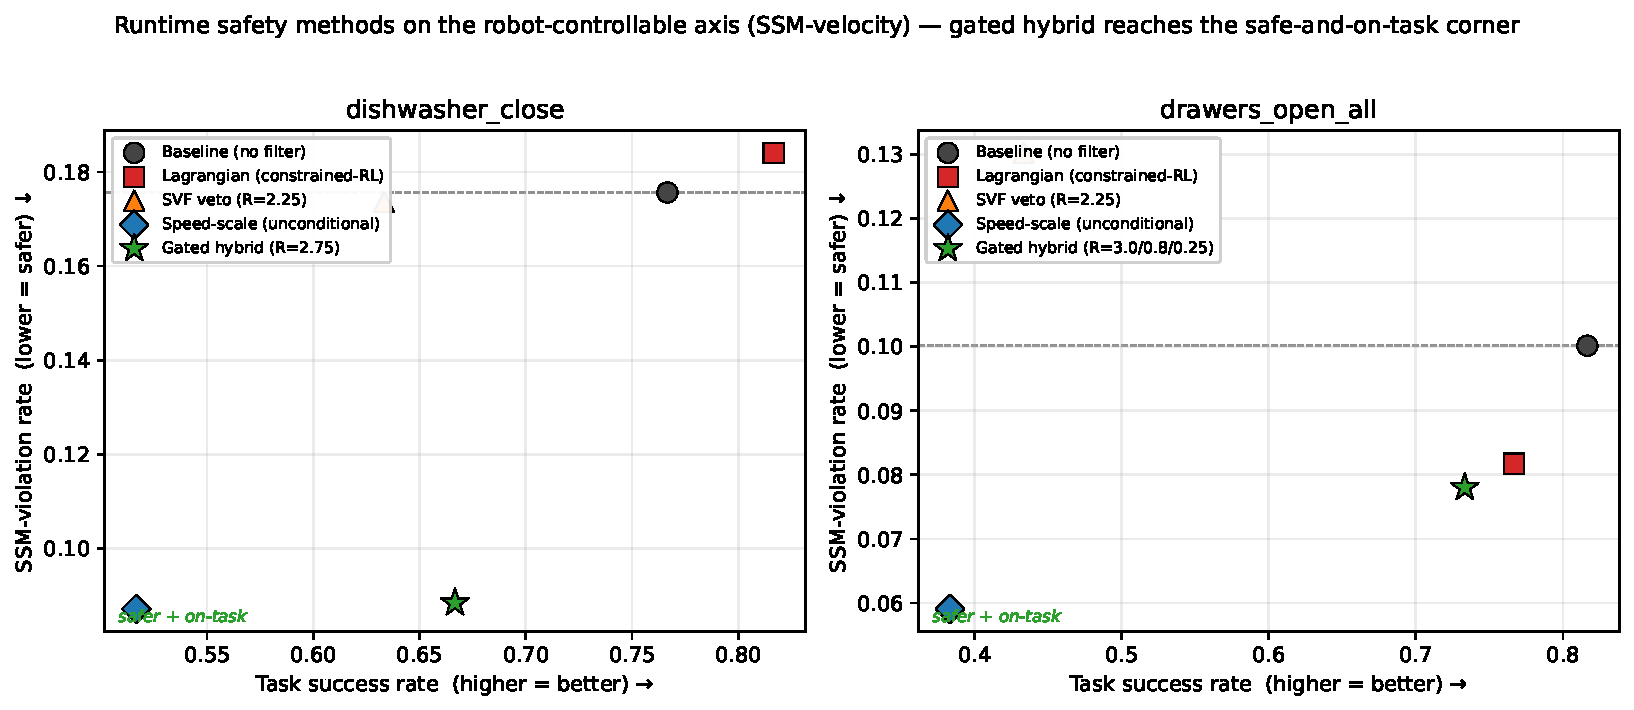
\includegraphics[width=0.75\textwidth]{fig1_method_comparison}
\caption{The intermittent-co-location headline: each method on the
success (x) / \ssm{}-violation (y) plane; the desirable corner is
bottom-right (high success, low violation), and only the
critic-gated filter reaches it on both tasks. Two points need their
context. The \emph{drawers Lagrangian} point sits near the gated
one, but it is a basin-selected checkpoint from seed-unstable,
single-seed training on which no feasible budget exists
(PID-$\lambda$ is inert or task-fatal across the budget sweep);
gating-on-Lagrangian $\approx$ gating-on-baseline (ablation~3,
Section~\ref{sec:results:r2-ablations}) shows it learned no
genuinely proactive avoidance; and it offers no deployable dial,
whereas the gate threshold $R$ traces a tunable frontier
(Figure~\ref{fig:r2-tradeoff}). The \emph{unconditional speed-scale}
points reach the lowest violation rates but at $2.5$--$5\times$ the
gated filter's success cost.}
\label{fig:r2-method-comparison}
\end{figure}

\begin{figure}[htbp]
\centering
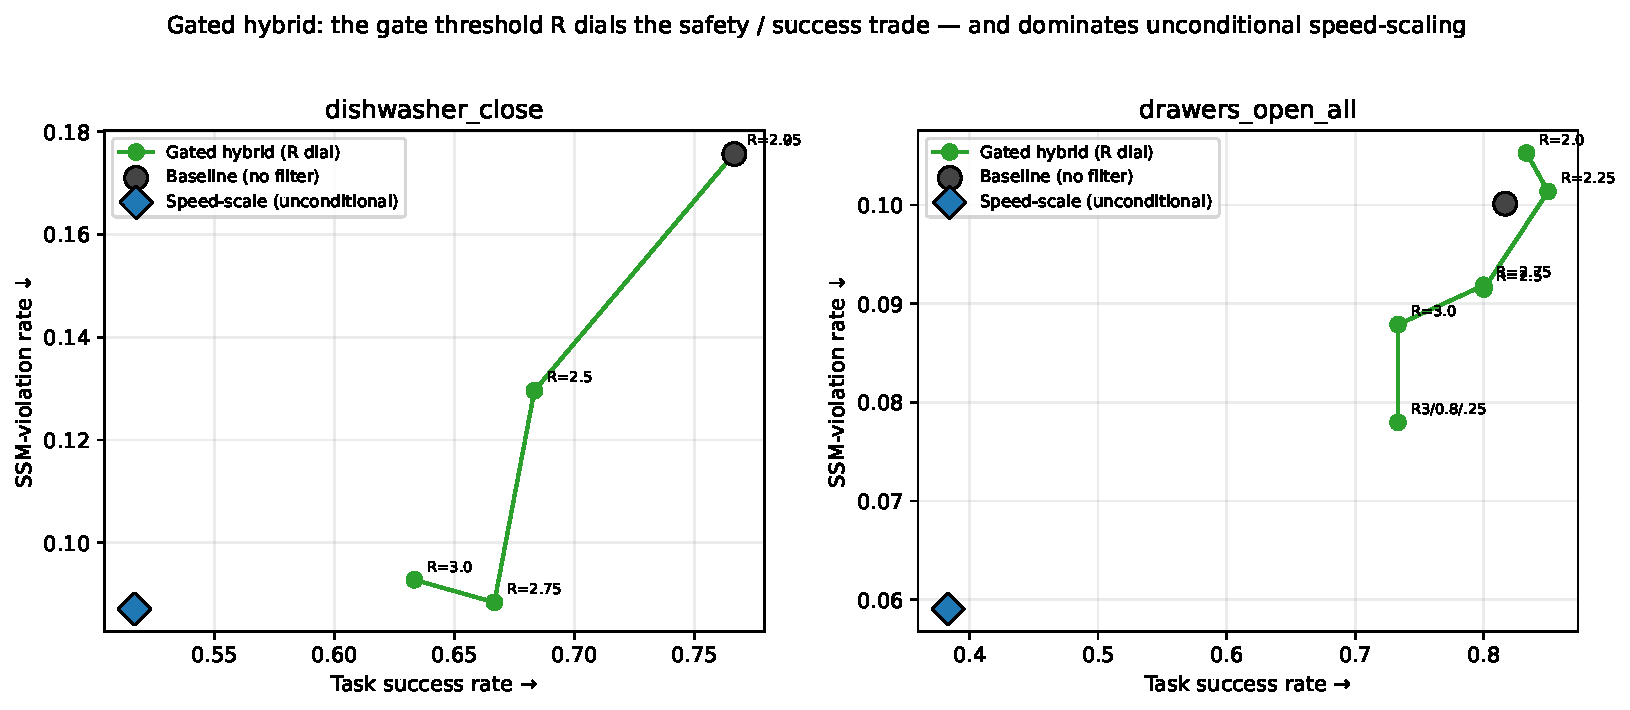
\includegraphics[width=0.7\textwidth]{fig2_tradeoff_curve}
\caption{The gate threshold $R$ is a clean operating-point dial: low
$R$ is selective (near-baseline success, small \ssm{} gain), high $R$
approaches unconditional scaling. The dominance claim is
task-scoped, per the two-axis protocol: on \emph{dishwasher} the gated
frontier matches unconditional scaling's \ssm{}-violation at
strictly higher success; on \emph{drawers} the gated frontier never
reaches unconditional's absolute floor ($0.059$ vs.\ best gated
$0.078$) but pays far less success at every \emph{shared}
\ssm{}-violation level.}
\label{fig:r2-tradeoff}
\end{figure}

The gated result should be read with its scope attached: the gate
recovers throughput \emph{where genuinely-safe windows exist for the
critic to find}. That scope is not a rhetorical hedge; it is the
regime variable, and Section~\ref{sec:results:boundary} measures it
and tests it on a third task.

\subsection{Gate Ablations: Four Refinements Confirm the Recipe}
\label{sec:results:r2-ablations}

Four follow-ups probed whether a better configuration was being
missed; all four converge back on the recommended recipe, and each
yields a portable lesson.

\begin{enumerate}[topsep=2pt,itemsep=2pt]
\item \emph{Pareto surface ($d_{\mathrm{slow}} \times R$,
  dishwasher).} Across $d_{\mathrm{slow}} \in \{0.4, 0.5, 0.6,
  0.8\}$\,m, the gate threshold $R$ is the dominant dial and
  $d_{\mathrm{slow}}$ is secondary ($R = 2.75$ gives $-49$ to
  $-51\,\%$ \ssm{} at $0.63$--$0.67$ success regardless). The
  $R$-sweep \emph{is} the frontier. One interaction matters:
  $R = 3.0$ with $d_{\mathrm{slow}} = 0.4$ re-introduces veto-like
  overshoot (max velocity $6.10$), so $d_{\mathrm{slow}} \geq 0.5$
  is kept, an echo of the veto's coherence break
  (Section~\ref{sec:results:r2-veto}) inside the gated filter
  itself.
\item \emph{Anticipatory critic labels.} Re-labelling the critic at
  looser thresholds ($0.20$ / $0.30$\,m, so it warns earlier) does
  not improve the operating point; the earlier-warning critics slide
  along the same success/safety trade (dishwasher $R = 2.75$:
  $0.63$/$-35\,\%$ and $0.63$/$-44\,\%$ vs.\ the $0.10$\,m critic's
  $0.67$/$-50\,\%$). The most \emph{selective} near-contact label is
  the best gate; anticipation belongs to the policy, not the gate.
\item \emph{Gating on the Lagrangian policy.} Running the gated
  backstop on the best Lagrangian basin checkpoint instead of the
  curriculum baseline is a wash (dishwasher $0.70$/$-36\,\%$ vs.\
  $0.67$/$-50\,\%$; drawers $0.77$/$-25\,\%$ vs.\ $0.80$/$-8\,\%$ at
  matched settings; neither dominates). This is the direct evidence
  that the budget-sweep Lagrangian produced no genuinely
  proactive-avoiding policy on these tasks, and it is what licenses
  the drawers-Lagrangian caveat on
  Figure~\ref{fig:r2-method-comparison}.
\item \emph{DAgger-style re-collection on filtered rollouts.}
  Retraining the critic on the \emph{filtered} policy's own rollouts,
  the natural ``fix the distribution shift'' move, is null to
  harmful: the re-collected critic \emph{under}-gates (dishwasher
  $-2\,\%$ \ssm{} vs.\ $-50\,\%$), because the filtered distribution
  already looks safe (the filter slowed the robot during
  collection), so the critic rarely fires. A runtime gate must be
  trained on the \emph{unfiltered} policy's behaviour: it has to
  recognise what the raw policy \emph{would} have done.
\end{enumerate}

\section{The Boundary Condition: One Law, Measured Across Three Tasks}
\label{sec:results:boundary}

The two preceding sections carry opposite headlines: on saucepan the
constrained policy is the working arm and every runtime filter pays
an unacceptable cost, while on dishwasher/drawers the critic-gated
filter is the working arm and constrained RL fails. The claim this
section establishes is that \emph{the two headlines are one finding,
and the variable that decides between them is measurable}. The
experiment that closes the loop is the cross-task gating test
(E4.4): run the exact intermittent-regime winner, critic-gated
speed-scaling, on \texttt{saucepan\_to\_hob}, under a decision rule
fixed in advance: \emph{the gate counts as recovering throughput iff
some threshold reaches success $\geq 0.60$ and \ssm{}-actual
$\leq 0.08$}.

\subsection{The Gate Does Not Recover Throughput on Saucepan}

Table~\ref{tab:e4.4-gated-saucepan} reports the full sweep (the
saucepan SVF critic, $R \in \{0 \ldots 3.0\}$, plus an on-policy
re-collected critic and the unconditional control; 180 episodes per
row). \textbf{No row passes the pre-registered rule.} As $R$ rises,
the operating point moves monotonically from policy-alone
($0.722$ success, $0.138$ \ssm{}-actual) to the unconditional point
($0.433$, $0.072$); the closest rows are $R = 3.0$ ($0.472$/$0.084$,
below the success floor) and $R = 2.5$ ($0.567$/$0.105$, below both
bars). The gated curve \emph{tracks} the unconditional scaler rather
than dominating it; no high-success, low-violation corner opens.
The decision rule failed on saucepan, and that outcome was the
\emph{predicted} failure mode under the regime map, not an anomaly to
be explained away.

\begin{table}[htbp]
\centering
\small
\caption{Experiment E4.4. Critic-gated speed-scaling on
\texttt{saucepan\_to\_hob} (180 episodes per row, 3 trained seeds;
\texttt{noisy}; \texttt{snapshot\_best} checkpoints, see the caveat
box). The pre-registered rule, success $\geq 0.60$ \emph{and}
\ssm{}-actual $\leq 0.08$, is met by no row: gating slides from
policy-alone toward the unconditional point without opening a
corner. The on-policy re-collected critic (v3op) does not help
either, at $R = 2.0$ its \ssm{}-actual ($0.149$) is \emph{worse}
than policy-alone ($0.138$), confirming the limit is task structure,
not critic calibration.}
\label{tab:e4.4-gated-saucepan}
\begin{tabular}{llcccl}
\toprule
Critic & $R$ & Success & Prox.\ viol. & \ssm{}-actual & Reads as \\
\midrule
v3      & 0.0  & 0.722 & 0.271 & 0.138 & policy alone (gate never fires) \\
v3      & 1.5  & 0.717 & 0.299 & 0.127 & gate barely active \\
v3      & 2.0  & 0.706 & 0.295 & 0.125 & \\
v3      & 2.5  & 0.567 & 0.282 & 0.105 & success falling \\
v3      & 2.75 & 0.472 & 0.275 & 0.102 & \\
v3      & 3.0  & 0.472 & 0.283 & 0.084 & approaching unconditional \\
uncond. & --   & 0.433 & 0.276 & 0.072 & the gate's $R \to \infty$ limit \\
v3op    & 2.0  & 0.733 & 0.297 & 0.149 & on-policy critic: no help \\
v3op    & 2.5  & 0.644 & 0.279 & 0.130 & on-policy critic: no help \\
\bottomrule
\end{tabular}
\end{table}

\begin{figure}[htbp]
\centering
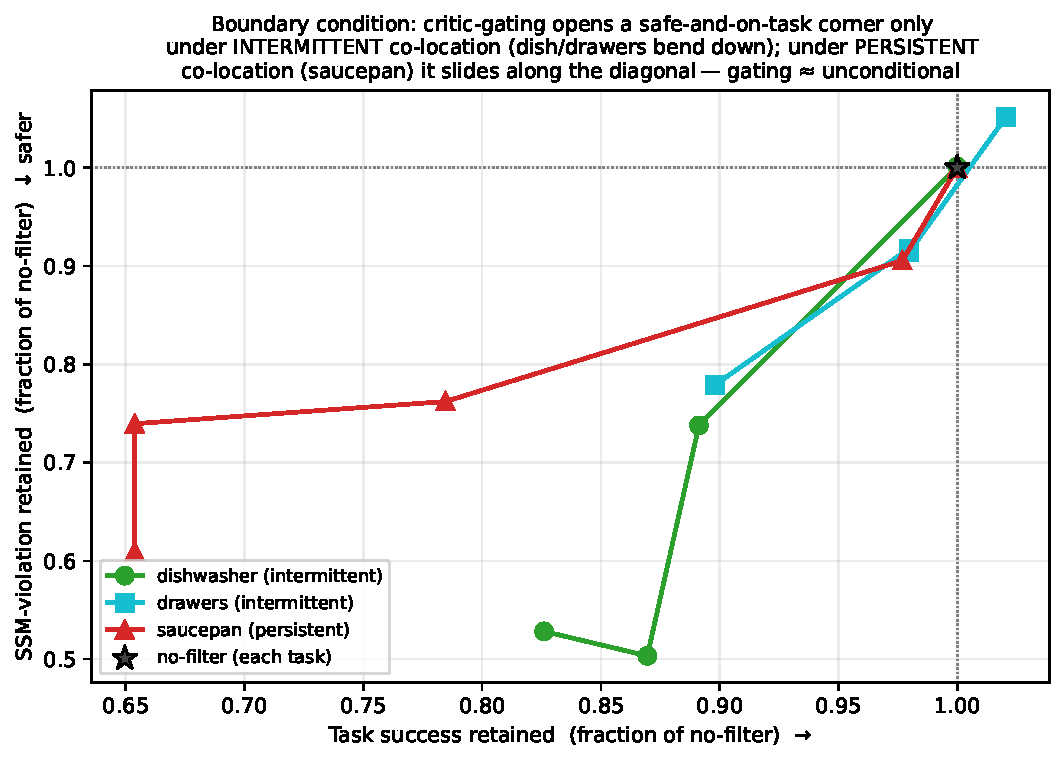
\includegraphics[width=0.72\textwidth]{fig5_cross_task_boundary}
\caption{The boundary condition in one picture: each task's gated
$R$-dial trajectory on the success/\ssm{}-violation plane,
normalised to its own no-filter point. Dishwasher and drawers
\emph{bend down}, \ssm{}-violation falls steeply while success is
retained, because the gate passes the genuinely-safe majority of
steps at full speed. Saucepan \emph{slides along the diagonal}
toward its unconditional endpoint, success and \ssm{}-violation
falling together, because the gate is active on most steps and
gating degenerates to unconditional scaling.}
\label{fig:cross-task-boundary}
\end{figure}

\subsection{The Mechanism, Measured}

The explanation is not asserted from task descriptions; it is read
off the gate itself (Figure~\ref{fig:gate-activity}). At the matched
threshold $R = 2.75$, the gate is active on $61.5\,\%$
$[57.2, 65.4]$ of steps on saucepan, versus $26.5\,\%$
$[16.3, 36.7]$ on dishwasher and $19.2\,\%$ $[12.7, 25.3]$ on
drawers; at each task's recommended operating point the contrast is
$51$--$63\,\%$ versus $\approx$27\,\%. On saucepan the gate fires
\emph{more often} than the unconditional scaler's own proximity
trigger ($44.2\,\%$ of steps within $d_{\mathrm{slow}} = 0.40$\,m):
the critic has no selectivity left to offer, so the ``gated'' filter
is the unconditional filter with extra steps. This is the same
mechanism the persistent-co-location section identified from the
other side, where the
\emph{unconditional} scaler's success floor was traced to a
separation-triggered response that ``fires almost constantly'' under
persistent co-location
(Section~\ref{sec:results:headline-feature-table}). The two arcs of
this report discovered one law from opposite directions:

\begin{quote}
\textbf{The boundary condition.} Critic-gated filtering recovers
task throughput if and only if human--robot co-location is
intermittent, because the gate's value \emph{is} the existence of
genuinely-safe windows to pass through at full speed. Under
persistent co-location no such windows exist, every
separation-triggered mechanism (gated or not) is active almost
continuously, and the only remaining lever on the exposure axis is
anticipatory avoidance, which must be trained into the policy.
\end{quote}

\begin{figure}[htbp]
\centering
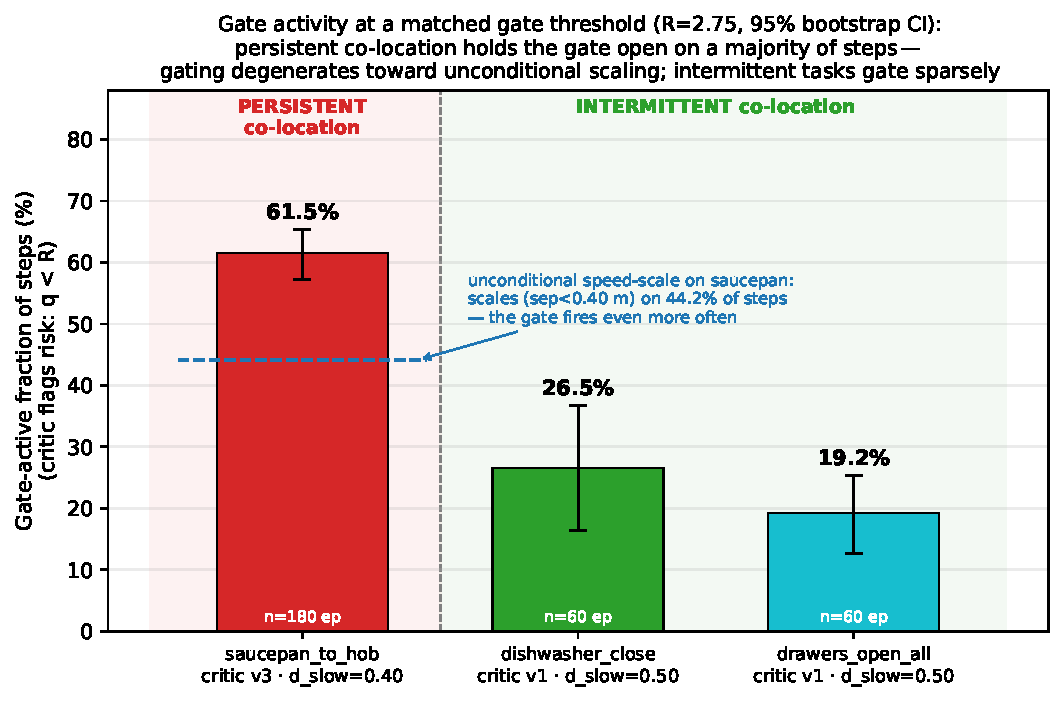
\includegraphics[width=0.58\textwidth]{fig7_gate_activity}
\caption{The regime variable, measured: per-step gate-active
fraction of the critic-gated filter at the matched threshold
$R = 2.75$ (bars; 95\,\% bootstrap CIs; 180/60/60 episodes). The
saucepan gate fires on $61.5\,\%$ of steps, exceeding even the
unconditional scaler's proximity trigger rate ($44.2\,\%$, dashed),
so gating degenerates to unconditional scaling; on
dishwasher/drawers the gate passes $73$--$81\,\%$ of steps at full
speed, which is exactly the recovered throughput of
Table~\ref{tab:r2-methods}.}
\label{fig:gate-activity}
\end{figure}

\subsection{The Regime Map}

Figure~\ref{fig:regime-map} assembles
the full cross-task picture. Two sentences in it are deliberately
blunt. First, \textbf{critic-gating does not rescue the saucepan
composition}: the policy--filter composition's $0.85 \to 0.44$
success cost (Section~\ref{sec:results:joint-coverage}) stands, an
on-policy critic does not change it, and the contribution of E4.4 is
the \emph{explanation} of that ceiling and its validation across
tasks, not a workaround for it. Second, the regime map is the
deployment rule: measure (or simulate) the co-location pattern
first, then pick the arm, a constrained policy where co-location is
persistent, a critic-gated backstop where it is intermittent, and
never a binary veto on a chunked policy.

\begin{figure}[htbp]
\centering
\begin{tikzpicture}[
  font=\small,
  regime/.style={draw, rounded corners, align=left, inner sep=7pt,
                 minimum width=0.43\textwidth, text width=0.40\textwidth},
  works/.style={text=green!45!black},
  fails/.style={text=red!60!black},
  lbl/.style={font=\small\bfseries, align=center},
]
\node[regime, fill=blue!4, draw=blue!50] (interm) at (0,0) {%
  \textbf{Intermittent co-location}\\[1pt]
  {\footnotesize \texttt{dishwasher\_close}, \texttt{drawers\_open\_all}}\\[1pt]
  {\footnotesize gate active on $\approx$19--27\,\% of steps}\\[4pt]
  {\footnotesize\textcolor{green!45!black}{\cmark\ critic-gated speed-scaling:
   $-50\,\%$/$-22\,\%$ \ssm{} at $\leq 0.10$ success cost}}\\[2pt]
  {\footnotesize\textcolor{red!60!black}{\xmark\ Lagrangian: no feasible budget
   (inert or task-fatal)}}\\[2pt]
  {\footnotesize\textcolor{red!60!black}{\xmark\ binary veto: chunk-coherence
   break (max vel $2.46 \to 6.03$)}}%
};
\node[regime, fill=orange!6, draw=orange!70!black, right=9mm of interm] (persist) {%
  \textbf{Persistent co-location}\\[1pt]
  {\footnotesize \texttt{saucepan\_to\_hob}}\\[1pt]
  {\footnotesize gate active on $\approx$51--63\,\% of steps}\\[4pt]
  {\footnotesize\textcolor{green!45!black}{\cmark\ constrained policy (fixed
   $\lambda$): $-23\,\%$ proximity at $0.76$ success}}\\[2pt]
  {\footnotesize\textcolor{red!60!black}{\xmark\ all reactive proximity filters:
   freeze or flee}}\\[2pt]
  {\footnotesize\textcolor{red!60!black}{\xmark\ critic-gating $\approx$
   unconditional scaling}}\\[2pt]
  {\footnotesize both-axis safety only via composition, at stacked cost
   ($0.85 \to 0.44$)}%
};
\draw[->, thick, black!60]
  ([yshift=-7mm]interm.south west) -- ([yshift=-7mm]persist.south east)
  node[midway, below=1mm, font=\footnotesize]
  {co-location persistence (measured: gate-active fraction, Figure~\ref{fig:gate-activity})};
\node[lbl, above=3mm of interm.north] {runtime arm carries safety};
\node[lbl, above=3mm of persist.north] {policy arm carries safety};
\end{tikzpicture}
\caption{The regime map (the thesis in one image). The observable
regime variable, how persistently the coworker is co-located,
measured as the fraction of steps a separation/risk-triggered filter
would be active, determines which arm of the Hybrid Safety Critic
carries the safety burden. The boundary was validated by the
pre-registered E4.4 rule, which failed on saucepan exactly as the
regime map predicted.
Evidence per cell: gated wins
(\S\ref{sec:results:r2-gated}), Lagrangian infeasibility
(\S\ref{sec:results:r2-lagrangian}), veto coherence break
(\S\ref{sec:results:r2-veto}), policy win and composition ceiling
(\S\ref{sec:results:headline-feature-table},
\S\ref{sec:results:joint-coverage}), freeze/flee taxonomy
(\S\ref{sec:results:reactive-taxonomy}), gating $\approx$
unconditional (Table~\ref{tab:e4.4-gated-saucepan}). On the
intermittent tasks the exposure axis itself is left without a
graceful mechanism, bounded by the exogenous floor
(\S\ref{sec:results:r2-lagrangian}).}
\label{fig:regime-map}
\end{figure}

\paragraph{Snapshot caveat (scope of the cross-task numbers).}
The exact persistent-task basin checkpoints were deleted in a
storage cleanup
before E4.4 ran; the sweep used each seed's
\texttt{snapshot\_best}, which peak-success selection makes
\emph{less} avoiding (its $R = 0$ row deploys at proximity $0.271$
vs.\ the basin's $0.228$). The verdict transfers for a measurable
reason: the unconditional control on \texttt{snapshot\_best}
reproduces the composition's success/velocity operating point
almost exactly ($0.433$/$0.072$ vs.\ $0.44$/$0.065$), and the gating
question is a statement about the \emph{filter} on exactly those two
axes; only proximity, the policy's axis, differs. A more-avoiding
basin policy would also leave the gate \emph{less} velocity to cut,
so any residual bias runs against gating helping more, not less. A
basin-checkpoint rerun requires retraining the three policies and is
recorded as a verification item, not a threat to the conclusion.

\section{Summary of Results}
\label{sec:results:summary}

\textbf{RQ1, the persistent regime: safety must be trained in.}
Where co-location is persistent, no runtime mechanism reduces
exposure gracefully: vetoes freeze, dodges flee, and every
separation-triggered filter is active on most steps. The
fixed-multiplier constrained policy cuts proximity violations by
$22.8\,\%$ ($0.296 \to 0.228$) at $0.76$ success across three seeds.
The reduction survives noisy, lagged perception and a held-out
coworker distribution ($-31\,\%$ there), while the worst-case
separation tail is exogenous, the coworker's own approach, and is
moved by no mechanism evaluated: proximity \emph{frequency} is
controllable, the single worst approach is not. Both axes at once
are available only by composing policy and graded scaler at a
stacked success cost ($0.85 \to 0.44$), the regime's ceiling.

\textbf{RQ2, the intermittent regime: gate the runtime backstop.}
Where encounters arrive in bursts, constrained RL finds no feasible
budget: the constraint is inert above the natural cost and
task-fatal below it, a binding multiplier makes motion \emph{faster}
(mean velocity $0.44 \to 0.79$\,m/s), and from-scratch WCSAC
corroborates the trainability difficulty externally. A binary veto
breaks chunked-policy coherence (max velocity $2.46 \to 6.03$\,m/s).
The working mechanism is the learned critic gating the graded
speed-scaler: $-50\,\%$ \ssm{}-violation at $-0.10$ success on
dishwasher, $-22\,\%$ at $-0.09$ (or $-10\,\%$ at $-0.02$) on
drawers, with the gate threshold as a deployable dial
(Figure~\ref{fig:r2-reduction-bars}).

\textbf{RQ3, the boundary: co-location persistence decides.} The
gate-active fraction separates the regimes cleanly ($61.5\,\%$ of
steps on saucepan versus $19$--$27\,\%$ on dishwasher/drawers at the
matched threshold), it predicts which arm carries the safety burden,
and the pre-registered cross-task rule failed exactly where the map
predicts: under persistent co-location, gating degenerates to
unconditional scaling, and constrained-RL feasibility flips across
the same boundary.

\begin{figure}[htbp]
\centering
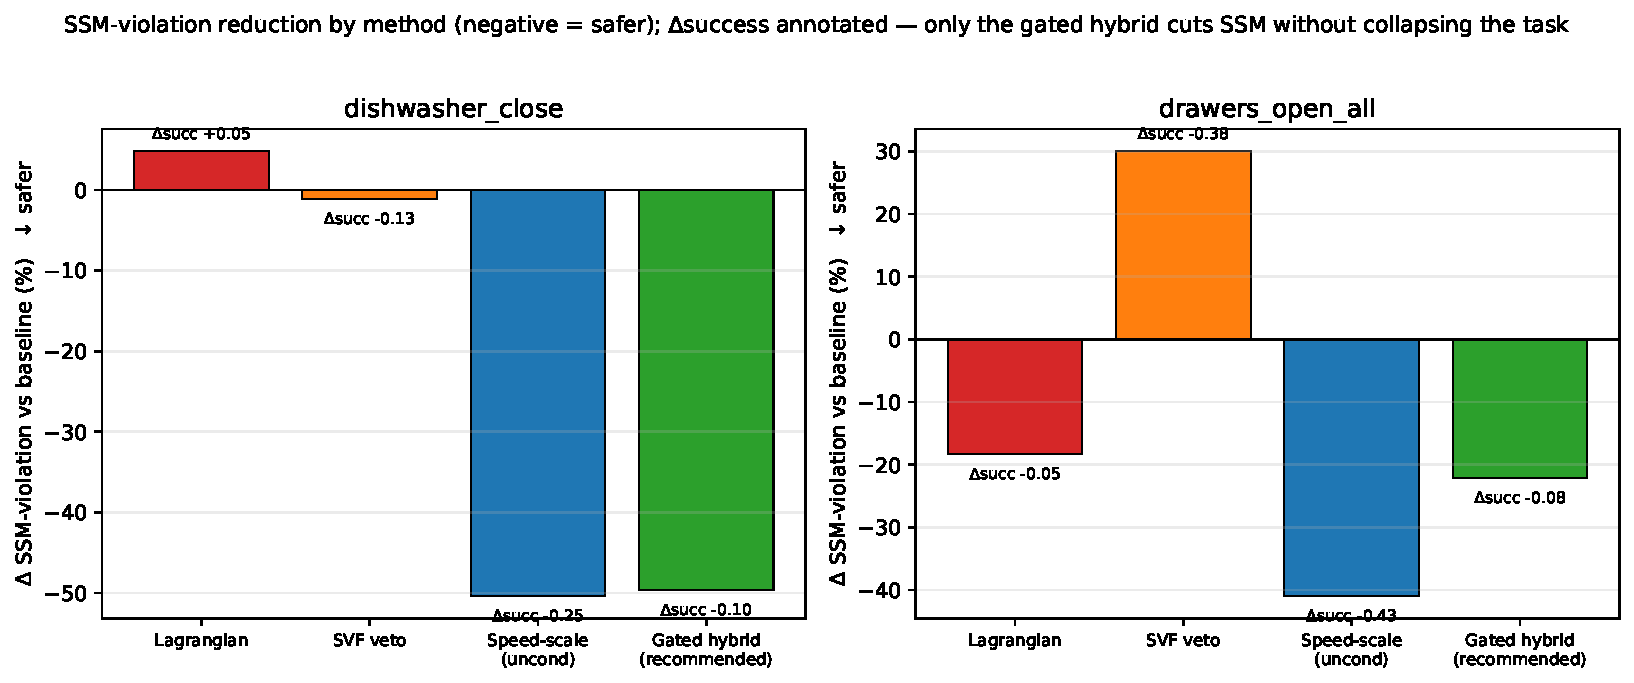
\includegraphics[width=0.7\textwidth]{fig3_reduction_bars}
\caption{Summary of the intermittent-co-location arm:
\ssm{}-violation reduction by method with the success cost
annotated. Only critic-gated speed-scaling combines a substantial
velocity-axis reduction with a small success cost; the unconditional
scaler buys slightly more reduction at several times the cost, the
veto and the Lagrangian buy little or none. The persistent-regime
counterpart of this figure is
Table~\ref{tab:e4.1-feature-incremental}.}
\label{fig:r2-reduction-bars}
\end{figure}
% =============================================================================
% PART V: DISCUSSION, FUTURE WORK, CONCLUSION
% =============================================================================

% =============================================================================
\chapter{Discussion}
\label{ch:disc}
% =============================================================================

\section{What the Answers Mean}
\label{sec:disc:rqs-revisited}

The factual answers to the three research questions are summarised
in Section~\ref{sec:results:summary}; this section adds the
interpretation that does not belong in a results table.

\textbf{On RQ1, the persistent regime.} Two points sit behind the
headline numbers. First, the observation pilot and the perception
sweep together say something sharper than either alone:
\emph{adding human-state observation to an imitation pipeline
without a safety-reward gradient is not a safety mechanism} (the
channel was inert or counterproductive under behaviour cloning), and
yet once a constraint gradient exists, the learned avoidance does
not depend on perfect state estimation (statistically
indistinguishable under \texttt{oracle} and \texttt{noisy}
perception). Imitation methods marginalise observations
uncorrelated with the demonstrated action; constrained RL has a use
for the channel. Second, the training lessons travel beyond this
benchmark: fix or schedule the multiplier when the only feasible
budget sits on a feasibility boundary, and select constrained
checkpoints by a safety-aware rule, because peak-success selection
picks \emph{against} the constraint.

\textbf{On RQ2, the intermittent regime.} \emph{Why} the same
constrained method flips from working to inert-or-fatal across
regimes admits a mechanism-level hypothesis, stated as discussion
rather than demonstrated result: persistent co-location makes the
cost signal \emph{dense} (nearly every step carries graded cost, so
the rolling cost moves smoothly and a feasible region exists just
below the inherent cost), while intermittent co-location delivers
cost in sparse bursts, leaving a cliff-shaped budget landscape
(inert on one side, windup on the other) with nothing graded for
the multiplier to push against. Base-task fragility compounds this,
as from-scratch WCSAC corroborates. Both halves are testable, and
the persistence dial (Section~\ref{sec:fw:persistence-dial}) is the
controlled test.

\textbf{On RQ3, the boundary.} The override form decides
feasibility, the gate decides cost, and the regime decides whether
the gate has anything to find. The honest claim is therefore not
``the hybrid dominates'' but ``each arm dominates its own regime,
and both-axis safety under persistent co-location has an explicit,
tunable price''. What no arm moves is the exogenous tail: proximity
\emph{frequency} is controllable, the single closest approach is
not, and only a Power-and-Force-Limiting collision brake
(Section~\ref{sec:fw:pfl}) could address it. The regime
classification itself rests on three tasks, a deliberate limitation
examined below (Section~\ref{sec:disc:regime-threat}).

\section{Threats to Validity}
\label{sec:disc:threats}

This section is deliberately frank: the work has well-defined
limits, and naming them precisely is part of the result, because
each one bounds where the regime map and the deployable recipes can
be trusted.

\subsection{The \pfl{} Contact-Detection Limitation}
\label{sec:disc:pfl-bug}

\textbf{The \iso{} compliance claim is qualified to ``geometric /
\ssm{}-only.''} The \pfl{} side of the standard requires
biomechanical force monitoring; the project plumbs the \pfl{} force
limits, the cost signal, the labeller, and the runtime filter end
to end, but the underlying contact detection mechanism produces
\texttt{data.ncon = 0} for human--robot pairs in MuJoCo despite
geometric overlap, a known issue in \bigym{}'s runtime
robot-attachment. Therefore $c^{\pfl}_t \equiv 0$ throughout this
work. \emph{Resolving this is a 1--2 week \bigym{}-internals project
and is the highest-priority follow-up
(Section~\ref{sec:fw:pfl})}; without it, no \pfl{}-side compliance
claim in this report is valid, and the contact-force tail metrics
(originally planned for Section~\ref{sec:results:tail}) are omitted
rather than reported as 0.

\subsection{Curriculum Dependence}
\label{sec:disc:curriculum}

The headline results presuppose the three-stage curriculum of
Section~\ref{sec:method:curriculum}. Direct training on the full
\coworker{} disruption collapses to evacuation; every headline
result generalises only to settings where a comparable staged
curriculum is feasible. This is not a fatal limit (curriculum
learning is a standard solution to long-horizon sparse-reward
RL~\cite{narvekar2020curriculum,openai2019solving,rudin2022walkminutes}), but it
should temper any reading of the architecture as ``trainable from
scratch on arbitrary human-co-located tasks.''

\subsection{Sim-to-Real: Three Orthogonal Gaps}
\label{sec:disc:sim2real}

\textbf{Perception:} the mock-\bodyslampp{} model is calibrated
against published characteristics~\cite{henning2023bodyslampp} but
is not real perception; a rendered-image run feeding a real
estimator is the natural closure
(Section~\ref{sec:fw:realbody}). \textbf{Dynamics:} MuJoCo's H1
differs from the real platform in unmeasured ways. Domain
randomisation~\cite{tobin2017domainrand,muratore2022randomized}
is the standard follow-up and remains the deployed recipe for
real-world humanoid RL~\cite{radosavovic2024humanoid}, and the gap
must be acknowledged before any real-world claim. \textbf{Contact
fidelity:} we found no validation of any rigid-body engine's contact
forces against measured human--robot collision forces.
Simulator validation on real impacts is trajectory-level only and
finds MuJoCo~\cite{todorov2012mujoco} nearly insensitive to its
contact-stiffness parameter~\cite{acosta2022simvalidation},
force-level MuJoCo validation exists only outside
HRC~\cite{joseph2026mujoco}, and industrial \pfl{} validation relies
on physical biofidelic measurement precisely because simulating
constrained contacts is considered
unreliable~\cite{schlotzhauer2022pfl,svarny2020collision}. The
benchmark's contact forces are therefore safety-shaped rather than
safety-validated, even once the \pfl{} detection limitation is
resolved.

\subsection{The Runtime Filter's Role Is Axis- and Regime-Conditional}
\label{sec:disc:filter-role}

The results force a precise statement of what a runtime filter
contributes, narrower than the field's default framing on one side
and broader on the other. \emph{Narrower}: on the proximity
(exposure) axis under persistent co-location, no reactive mechanism
helps gracefully, the fallback sub-study
(Section~\ref{sec:results:filter-pareto}) shows the only
proximity-cutting fallback is a task-abandoning retreat that worsens
the \ssm{}-actual rate, and this freeze-versus-flee limit is one the
runtime-filter literature reaches independently
(Section~\ref{sec:bg:cbf:conservatism}): a worst-case reactive
filter over-restricts to stay safe~\cite{tian2022confidence},
relaxing conservatism is provably benign only for a
least-restrictive filter~\cite{permissivefilter2025}, and trusting a
human-motion model to relax it fails exactly when the human is
unpredictable~\cite{tian2022confidence}, as a co-located coworker
is. The internalisation analysis
(Section~\ref{sec:results:interaction}) adds the composition half: a
learned veto's intervention rate does not fall as the policy learns
to avoid, it rises, because the avoiding policy exits the critic's
calibration distribution. \emph{Broader}: on the velocity axis with
the right override form, the filter is not a backstop but the
\emph{primary} working mechanism wherever co-location is
intermittent, the critic-gated scaler is the best operating point in
the entire evaluation there, and even under persistent co-location
the unconditional scaler is the only route to velocity-axis
compliance, at a price the regime sets. Our contribution is to
establish both halves empirically on a high-DOF manipulator under
\iso{}, and to name the variable that separates them. The reading is
calibrated on the \coworker{} distribution and these base policies; a
distribution with more robot-initiated approaches would shift the
exogenous share and require re-calibrating filter operating points
($R$, $d_{\mathrm{slow}}$) against the deployed policy.

\subsection{Generalisation Scope and the Resolved Cross-Task Transfer}
\label{sec:disc:arch-gen}

The constrained-RL evidence supports the claim that, on the
persistent-co-location task under this backbone, a fixed-$\lambda$
Lagrangian at a feasible budget achieves a reproducible proximity
reduction where both auto-tuned budgets and reactive filters do not
(RQ1). The cost-form ablation bounds the scope: the cost-signal
\emph{form} (continuous vs.\ binary) is not the operative variable,
the budget relative to the task's inherent cost is, so we do not
claim a general ``continuous beats binary'' result. \emph{Cross-task
transfer} of the full saucepan pipeline (E5.3) resolved
\emph{negative}: on \texttt{dishwasher\_close} and
\texttt{drawers\_open\_all} no budget binds usefully and the best
constrained point is within noise
(Section~\ref{sec:results:r2-lagrangian}). Under the regime map this
negative is informative rather than anomalous, but its converse
limits should be stated equally plainly: ``reproducibly'' in the
persistent-regime headline means across three saucepan training
seeds, not across
tasks; and whether the fixed-$\lambda$ recipe holds under a
different backbone, a one-shot-intrusion disruption pattern, or a
different embodiment remains untested.

\subsection{External Baseline (WCSAC): Implemented, with Stated Limits}
\label{sec:disc:wcsac-honest}

The WCSAC~\cite{yang2021wcsac} comparison
(Section~\ref{sec:results:wcsac}) is reported with four explicit
limits. (i) \emph{Single seed per cell}: from-scratch SAC is
high-variance, and the anomalous dishwasher $d{=}30$ cell ($0.03$
success at $\lambda = 0$) is best read as that variance, not as a
budget effect; a clean WCSAC trade-off curve needs $\geq 3$ seeds.
(ii) \emph{From-scratch by necessity}: WCSAC is actor-critic and
cannot consume the critic-only warm-start snapshots, so the
comparison conflates ``safe-RL formulation'' with ``demonstration
prior'', which is exactly why it is presented as an external
reference for trainability and not as a like-for-like ablation.
(iii) \emph{Oracle perception at evaluation}, an upper bound with
respect to the noisy condition the project's own methods are
evaluated under. (iv) \emph{No Safety-Gym revalidation}: the
reimplementation was cross-validated against the training-time
evaluator on these tasks (and a de-normalisation confound was found
and fixed before any number was recorded,
Section~\ref{sec:method:wcsac}), but it was not re-run on Safety-Gym
to reproduce published numbers, so residual reimplementation error
cannot be fully excluded. Within those limits the result is robust:
WCSAC's dishwasher success demonstrates the external method is
viable on the easier task, and its uniform drawers failure
corroborates the base-task-fragility reading of the budget-retarget
result (Section~\ref{sec:results:r2-lagrangian}).

\subsection{The Regime Classification Is Observational, on Three Tasks}
\label{sec:disc:regime-threat}

The regime map rests on three tasks, and the regime variable is
\emph{measured} but not \emph{manipulated}: persistence co-varies
with task identity, geometry, episode length, and policy speed, so a
confound-free causal reading is not yet available. Three things
mitigate, without eliminating, the concern: the boundary condition
was pre-registered before the cross-task gating test ran (the
saucepan failure case is a prediction satisfied, not a post-hoc
classification); the mechanism
is measured at the step level (Figure~\ref{fig:gate-activity}), and
the degeneration it implies is visible \emph{within}-task as $R$
rises (Table~\ref{tab:e4.4-gated-saucepan}); and the same boundary
predicts an unrelated phenomenon, the constrained-RL feasibility
flip, which a task-identity explanation would have to explain
separately. The clean falsification test is the \emph{persistence
dial} (Section~\ref{sec:fw:persistence-dial}): hold the task fixed,
manipulate only the coworker's dwell schedule, and watch whether the
dishwasher's bent frontier flattens onto the diagonal. Until it
runs, the regime map should be read as a strongly-evidenced
empirical regularity with a measured mechanism, not a proven causal
law.

\subsection{Headline-Architecture Caveat (B-value-mean vs.\ B-CVaR)}
\label{sec:disc:arch-caveat}

The headline architecture is B-value-mean (mean-cost dual-critic).
The standard critique of mean-cost Lagrangian methods is that they
bound only $\mathbb{E}[Z_c]$, not the tail~\cite{yang2021wcsac}. We
report $\cvar_{0.95}$ as a diagnostic and find that the mean-trained
policy's worst-case separation tail is no worse than the baseline's,
but the reason is specific to this setting and does \emph{not} vindicate
mean-cost training in general: the tail here is \emph{exogenous}
(Section~\ref{sec:exogenous}), the human walking into a co-located
robot, so it lies outside what \emph{any} robot-side training
objective, mean or CVaR, can move. A CVaR-trained policy would not
reduce this tail either; the limitation is the reactive control
surface, not the risk measure. On a heavier-tailed cost distribution
whose tail \emph{is} robot-driven (explicit adversarial coworker
behaviours, contact-rich tasks where the robot's own motion creates
the worst case), the mean-trained policy would likely under-perform a
CVaR-trained one, and the future-work direction
(Section~\ref{sec:fw:cvar}) is motivated by that scenario rather than
by this one.

\subsection{Computational Feasibility}
\label{sec:disc:compute}

At 76 DOF, a constraint-projection CBF quadratic program would have to
be constructed and solved over many human-link pairs every control
step, a substantially heavier per-step cost than a single MLP forward
pass and one that additionally requires hand-specified barrier
functions; this project instead uses a learned safety value function
(for the veto) and a closed-form speed-scaling rule as the runtime
filters, both of which are negligible alongside the policy's own
forward pass. The control loop runs at 20\,Hz (a 50\,ms per-step
budget); the policy forward pass, the filter evaluation, and the
fallbacks are simple tensor operations that sit comfortably within
that budget, so no component was separately micro-profiled. The
substantive computational argument is comparative: the learned
filter avoids the per-step QP that a 76-DOF CBF would demand.

\section{Broader Impact}
\label{sec:disc:broader}

\subsection{Responsible Deployment and Misuse Risk}

The strongest practical implication of the regime map is also the
largest ethical warning: a runtime safety wrapper can make a learned
humanoid \emph{look} safer without making it certifiably safe. The
project improves measurable \ssm{}-velocity behaviour in simulation,
but it does not validate real contact forces, real perception
failures, or real human reactions. A company deploying a humanoid in a
home, warehouse, or care setting could misuse these results by
presenting a wrapper as evidence of ISO compliance. That would be a
category error. The report's claim is narrower: the mechanisms improve
specific measured axes in a simulated co-working benchmark, and the
\pfl{} force loop remains unevaluated.

The regime map adds one concrete pre-deployment check: \emph{measure
the co-location pattern first}. The gate-active fraction of a candidate
filter on logged or simulated traffic is cheap to compute and, on this
evidence, predicts whether critic-gated scaling can recover throughput
or whether persistent co-location will force a heavy safety--throughput
trade. This should be treated as a screening test, not a certificate.
If the pattern is persistent, a deployer should expect either slowed
operation, proactive task replanning, or a redesign of the workspace
rather than a transparent safety layer.

A second lesson, from E4.3, is that validation must be joint. A runtime
filter cannot be assumed to ``hand over'' to a policy trained to be
safe, because the policy may move out of the critic's calibration
distribution. Real-world validation must therefore test the exact
policy--filter composition on the exact deployment distribution, with
the filter re-calibrated whenever the policy, perception stack, task,
or coworker pattern changes.

\subsection{Vulnerable Users and Domestic Environments}

\iso{} targets industrial collaboration, where users are trained,
adult, aware of the robot, and operating under a safety process.
Domestic or care environments violate those assumptions. Children may
approach unpredictably, elderly users or disabled users may have slower
reaction times, and bystanders may not understand the robot's intended
workspace. The exogenous-proximity finding is therefore especially
important: if a vulnerable person walks into a stationary robot, a
robot-side policy cannot remove the exposure, and only a last-resort
\pfl{} brake, physical workspace design, supervision, or external
sensing can reduce the residual risk.

For this reason the report should not be read as a case for deploying
learned humanoid manipulators in unconstrained homes. It is a step
towards evaluating such systems. Extending it to vulnerable-user
deployment would require stricter cost budgets, real BodySLAM++ or
multi-camera perception tests, contact-force validation, emergency-stop
hardware, human-subjects ethics review, and a regulatory answer to
which standard applies outside the industrial-collaboration setting.
The safety--throughput trade should also be disclosed to users: in the
persistent regime, the safer configuration may be substantially slower
or less successful, and hiding that cost would encourage unsafe
expectations about what the robot can do.

\subsection{Reproducibility as Honesty}

The full reproducibility checklist (Appendix~\ref{app:repro})
documents commit hashes, hyperparameters, dataset versions, and GPU
hours per phase, and the codebase is open-source under the MIT
licence at \url{https://github.com/ayushpatel4/safety-bigym-2},
together with the \bigym{} fork carrying the collision-channel and
PD-actuator fixes (patches submitted upstream). This is a small but
non-zero contribution to the safe-RL community's reproducibility
crisis.


% =============================================================================
\chapter{Conclusions and Future Work}
\label{ch:conclusion}
% =============================================================================

\noindent
\iso{}-referenced safety for high-DOF humanoid manipulation under
human co-working has not been systematically addressed in the safe-RL
literature. The field has strong ingredients, including constrained
RL and runtime filtering, but it did not have a rule for when each
should be used. This work contributes five linked pieces, in the
order of the introduction: the regime map, an empirical rule for
matching the safety mechanism to the human--robot co-location
pattern; a two-axis measurement protocol built on the finding that
$\approx$42\,\% of close proximity is human-driven and therefore
outside robot control; \sbigym{}, a safety-aware extension of the
\bigym{}~\cite{chernyadev2024bigym} benchmark on which the question
can be asked at all; a value-based re-derivation of the constrained
objective for critic-only agents, with a proved C51 support-bound
condition for dense shaping; and a set of mechanism-level design
lessons with deployable operating points.

\noindent
Which mechanism helps is governed by the human--robot co-location
regime, not by mechanism sophistication. Under \emph{persistent}
co-location (\texttt{saucepan\_to\_hob}, gate-active
$\approx$62\,\% of steps), only the anticipatory constrained policy
reduces exposure gracefully: a fixed $\lambda = 0.1$ value-based
Lagrangian cuts the proximity-violation rate by $22.8\,\%$
($0.296 \to 0.228$) at $0.76$ success across three seeds, where PID
auto-tuning is seed-unstable at the feasibility boundary; every
reactive filter pays a freeze-or-flee cost on that axis, and both
measured safety axes are improved only by composing policy and graded
speed-scaling at a multiplicative success cost ($0.85 \to 0.44$).
Under
\emph{intermittent} co-location (\texttt{dishwasher\_close},
\texttt{drawers\_open\_all}, gate-active $19$--$27\,\%$),
constrained RL finds no feasible budget, and when its multiplier
binds the robot gets \emph{faster}, not safer, with the from-scratch
WCSAC~\cite{yang2021wcsac} reference corroborating the trainability
difficulty. A binary veto breaks chunked-policy coherence (max
velocity $2.46 \to 6.03$\,m/s), and the working mechanism is a
learned critic \emph{gating} an \iso{} speed-scaling backstop:
$-50\,\%$ \ssm{}-violation at $-0.10$ success on dishwasher,
$-22\,\%$ at $-0.09$ on drawers, with the gate threshold as a
deployable dial.
The boundary was validated by a pre-registered rule whose failure case
occurred on saucepan, where gating measurably degenerates to
unconditional scaling. The worst-case separation tail is
exogenous and unmoved by every mechanism: exposure frequency is
controllable; the single closest approach is not.

\noindent
As humanoid platforms move from research labs into commercial
deployment (and the Unitree G1's deployment without
collaborative-operation validation~\cite{unitree_g1,hartmann2026iso}
is a representative data point),
principled methods for safety under imperfect perception and
sustained human co-presence are urgently needed. The most useful
output of this work is a decision rule where the field had only a
default. Runtime filtering is not a universal safety layer, and
constrained RL is not a universal alternative. The co-location
pattern, cheap to measure on logged or simulated traffic, predicts
which arm is likely to work and what the safety--throughput trade will
cost. The positioning table
(Table~\ref{tab:related-work-comparison}) situates the work honestly
within the emerging literature rather than claiming primacy. The
practitioner lessons are concrete: gate the scaler, do not veto a
chunked policy; train the gate critic on unfiltered rollouts; fix the
multiplier when the feasible budget lies on a boundary; select
constrained checkpoints by a safety-aware rule; and check the
support-bounding invariant before adding dense shaping to a
distributional critic.


\section{Future Work}
\label{ch:future}
\label{sec:conclusion:fw}

\subsection{The Persistence Dial: From Regime Map to Causal Test}
\label{sec:fw:persistence-dial}

The single highest-value next experiment, and the named next step of
this project. The regime map currently rests on three tasks in which
co-location persistence co-varies with task identity
(Section~\ref{sec:disc:regime-threat}). The persistence dial removes
the confound: hold the task fixed (\texttt{dishwasher\_close}, the
cheapest), and run the \emph{same} gated $R$-sweep under two
scripted-coworker schedules, the existing intermittent patrol and a
persistent variant in which the coworker's near-zone dwell is
extended to span the episode. The map makes a falsifiable
prediction: the dishwasher's bent frontier
(Figure~\ref{fig:cross-task-boundary}) flattens onto the diagonal as
the gate-active fraction rises toward the saucepan range, with the
transition tracking the measured gate activity rather than any task
property. A confirming result upgrades the boundary condition to a
controlled intervention on the regime variable; a disconfirming one
localises what task identity contributes. The infrastructure exists
(the dwell knobs are \texttt{ParameterSpace} axes,
Table~\ref{tab:coworker-params}); the cost is one gated sweep per
schedule.

\label{sec:fw:proactive}%
A companion question on the same tasks: the intermittent regime's
\emph{exposure} axis is left without a working mechanism (the
Lagrangian is inert or task-fatal there, and the gate by design does
not reduce exposure). The open lever is a potential-based separation
reward, which sidesteps the budget-cliff mechanism entirely. The
equally concrete risk is that the task geometry (the robot must
occupy the appliance the coworker walks through) imposes its own
exposure ceiling, in which case the honest outcome is a measured
ceiling rather than a win. Either result sharpens the regime map's
exposure column.

\subsection{Closing the Force Loop: Fixing \pfl{}}
\label{sec:fw:pfl}

The highest-priority infrastructure follow-up. Fix \bigym{}'s runtime
robot-attachment to expose human--robot contacts via
\texttt{data.ncon}, then re-run the pipeline with
\texttt{use\_pfl=true}. Estimated effort: 1--2 weeks of focused
\bigym{}-internals work. Until this is done, the project's \iso{}
compliance claim is \ssm{}-only; with it, the full standard is in
scope, and a \emph{last-resort collision-imminent brake}, firing only
at near-contact, becomes evaluable. That brake is the only mechanism
class that could address the exogenous near-contact tail that no
current mechanism moves (Section~\ref{sec:results:tail}),
completing the division of labour:
policy $\to$ exposure, filter $\to$ velocity, \pfl{} brake $\to$
contact. The schema is forward-compatible: the labeller, cost signal,
and runtime filter all read $c^{\pfl}_t$ unconditionally.

\subsection{Stronger Guarantees: \cvar{} Training and Formal Filters}
\label{sec:fw:cvar}
\label{sec:fw:formal}
\label{sec:fw:fallback}
\label{sec:fw:filter-during-training}

On the training side, the mean-cost headline formulation lifts to an
explicit distributional cost critic
(Section~\ref{sec:method:lagrangian:Bcvar}): a Gaussian
parametrisation (WCSAC-style~\cite{yang2021wcsac}) or quantile head
(QR-DQN-style~\cite{dabney2018qrdqn}), with ready instruments in
off-policy trust-region \cvar{} constraints~\cite{kim2022offtrc} and
distributional multi-constraint methods~\cite{kim2023sdac}. The cost
critic is already C51-shaped, so a parallel head slots in cleanly,
subject to the support invariant of
Proposition~\ref{lem:support-bound} holding for the cost
distribution. The motivating scenario is a cost tail that is
\emph{robot-driven} (contact-rich tasks, adversarial coworkers); on
the current benchmark the tail is exogenous and no risk measure can
move it (Section~\ref{sec:disc:arch-caveat}).

On the runtime side, our filters demonstrate velocity-axis behaviour
empirically but certify nothing. A CBF-QP with a certified barrier
or an HJ-reachability
filter~\cite{bansal2017hamilton,hsu2024safetyfilter} would add
provable separation/velocity guarantees; the concrete obstacles are
a control-affine dynamics model under \emph{exogenous} human motion
and the curse of dimensionality at 76 DOF, and the well-posed target
is the velocity axis, where the filter's role is unambiguous. The
sharpest unmeasured design, surfaced by the literature survey behind
Section~\ref{sec:bg:cbf:conservatism}, combines confidence-aware
fallback~\cite{tian2022confidence} with this report's override
finding: an \emph{anticipatory filter whose conservative fallback is
graded slow-down rather than freeze}, trusting a human-motion model
only under online misspecification monitoring. We found no published
work that measures that combination. Two smaller items complete the
thread: a proportional-damping fallback where a veto is unavoidable,
and the implemented-but-unrun filter-during-training ablation
(Section~\ref{sec:method:lagrangian:filter-train}), expected to
trade fewer catastrophic exploration trajectories for some
robustness cost~\cite{cbfrl2024,shield2025}.

\subsection{Real-Robot Transfer and the Coworker Realism Spectrum}
\label{sec:fw:realbody}
\label{sec:fw:embodiment}

The large-scale extension: a real Unitree~H1, real
\bodyslampp{}~\cite{henning2023bodyslampp} from on-robot RGB + IMU,
and real human collaborators under ethics review with a safety
supervisor in the loop; the project contributes the calibrated noise
model, the regime map, and the curriculum, and the open question is
whether the map survives deployment. Two cheaper studies sit on the
way: a \emph{coworker-aggressiveness spectrum} (the
\texttt{coworker\_eval} axes swept continuously), charting where
reactive filtering becomes sufficient as the human grows less
adversarial, and an SMPL-H~\cite{romero2017smplh} coworker
replication of the headline cells via the benchmark's body-agnostic
selector (Section~\ref{sec:bench:human}), a $\sim$15 GPU-hour check
on embodiment-specificity.


% =============================================================================
% Declarations (departmental requirement; unnumbered, before references)
% =============================================================================
\clearpage
\chapter*{Declarations}
\addcontentsline{toc}{chapter}{Declarations}

\paragraph{Originality.}
I declare that this report and the work it describes are my own,
carried out under the supervision of Dr Stephen James, and that all
material from other sources, published or unpublished, is
acknowledged and cited in the references.

\paragraph{Use of generative AI.}
Generative AI tools were used as assistive tools for literature search,
code scaffolding, experiment-log summarisation, plotting-script drafts,
\LaTeX{} formatting, and prose drafting/proofreading. They were not
used as an autonomous source of experimental results or as a substitute
for authorial judgement: all citations were checked against primary
sources, all correctness-bearing code was reviewed and tested by the
author, all numerical claims were traced to run logs or CSV artifacts,
and all report prose was edited and endorsed by the author. The full
declaration, including observed failure modes and verification
procedures, is in Appendix~\ref{app:genai}.

\paragraph{Ethics.}
The project involves no human-subjects research and no personal
data; all human-motion data is from the publicly released AMASS
dataset under its research licence. The full ethical considerations,
including the principal risk of over-claiming safety compliance, are
in Appendix~\ref{app:ethics}.

\paragraph{Sustainability.}
Total compute was roughly 450--500~GPU-hours on A100s,
corresponding to approximately 40\,kg~CO\textsubscript{2}e; the
accounting and the practices that bounded it are in
Appendix~\ref{app:sustainability}.

\paragraph{Code and data availability.}
The code is open-source under the MIT licence at
\url{https://github.com/ayushpatel4/safety-bigym-2}; model-weight and
dataset availability are detailed in Appendix~\ref{app:data}.

% =============================================================================
% References
% =============================================================================
\clearpage
\phantomsection
\addcontentsline{toc}{chapter}{Bibliography}
\bibliography{references}

% =============================================================================
\appendix
% =============================================================================

\chapter{Hyperparameter Tables}
\label{app:hparams}

\section{Phase 2: Offline CQL Safety Critic}
\label{app:hparams:svf}

\begin{table}[htbp]
\centering
\small
\caption{Phase 2 offline CQL safety-value-function hyperparameters.
The dataset is collected under \texttt{noisy} perception because a
runtime filter must learn the conditions it faces at deployment
(Section~\ref{sec:setup:perception-mode}).}
\label{tab:app-hparams-svf}
\resizebox{\textwidth}{!}{%
\begin{tabular}{lll}
\toprule
Hyperparameter & Value & Note \\
\midrule
Architecture & MLP $[256, 256, 256]$ $+$ scaled sigmoid & bounded value head \\
Optimiser & Adam, lr $3\times 10^{-4}$ & \\
CQL regulariser & $\alpha_{\mathrm{CQL}} = 5.0$ & ablated in E2.1 \\
Target violation rate & $0.30$ & matches $\tau_{\mathrm{prox}}$ calibration \\
Discount & $\gamma = 0.99$ & \\
Target-net Polyak & $\tau = 0.005$ & \\
Dataset & v3: \cqnas{} rollouts, \texttt{coworker\_train}, \texttt{noisy} & labelled at $\tau_{\mathrm{prox}}{=}0.3$\,m ($\sim$16.8\,\% unsafe) \\
Sampler & violation-balanced, target $1{:}1$ & \\
Training / batch & 200{,}000 steps / 512 & \\
\bottomrule
\end{tabular}%
}
\end{table}

The four collection-versus-deployment faithfulness fixes that make
this critic's deployment decisions valid (action de-normalisation,
execution-mode matching, the $500 \rightarrow 20$\,Hz control-frequency
root cause, and coworker-scenario alignment) are described in
Section~\ref{sec:impl:svf-faithful}; the $R = 0$ sweep agreement
($0.286 \approx 0.296$) is the validation that the fixes succeeded.

\section{Phase 3: Constrained Lagrangian Agent (Headline: Fixed $\lambda$)}
\label{app:hparams:lagrangian}

Table~\ref{tab:app-hparams-lagrangian} gives the headline
configuration. The headline multiplier is \emph{fixed} at
$\lambda = 0.1$; the PID gains below are used \emph{only} for the
E3.2 auto-tuning runs that establish the seed-instability finding
(Section~\ref{sec:results:budget}), and are set to zero for the
headline. There is no active cost budget $d$ in the headline, because
pinning $\lambda$ removes the dual-update loop entirely; $d = 0.3$ is
the budget used in the PID-ablation runs.

\begin{table}[htbp]
\centering
\small
\caption{Phase 3 headline hyperparameters (fixed-$\lambda$
constrained \cqnas{}). The cost critic is fully decoupled (its own
optimiser and its own features, the RoboBase shared-encoder
constraint) and cold-started.}
\label{tab:app-hparams-lagrangian}
\resizebox{\textwidth}{!}{%
\begin{tabular}{lll}
\toprule
Group & Value & Note \\
\midrule
\cqnas{} backbone & C51, 101 atoms, $\gamma = 0.99$ & \cite{seo2024cqnas} \\
Value support & $v_{\min} = -6$, $v_{\max} = +2$ & satisfies Prop.~\ref{lem:support-bound} \\
Cost critic & mirrored C51, same support & decoupled optimiser \& features; cold-started \\
Replay / batch / stack & 1M / 256 / 4 & \\
Demonstrations & $\text{num\_demos} = 36$ & \\
\textbf{Multiplier (headline)} & \textbf{fixed $\lambda = 0.1$} & dual loop removed \\
PID gains (E3.2 ablation only) & $K_I{=}10^{-3}, K_P{=}10^{-2}, K_D{=}0$ & $\lambda_{\max}{=}100$; zero in headline \\
Cost budget (E3.2 ablation only) & $d = 0.3$ & not active in headline \\
Workspace shaping & $\beta{=}0.05, r_{\mathrm{ws}}{=}0.4$\,m, $c_{\mathrm{ws}}{=}1.0$\,m & confound-controlled (E4.1) \\
Lagrangian fine-tune & up to 40{,}000 frames & on the stage-2 base \\
Checkpoint selection & \textbf{safety-aware} & lowest deploy proximity at success floor $0.75$ \\
Eval interval & 2{,}000 frames, 20 eval ep & basin at $\sim$20k--35k frames \\
\bottomrule
\end{tabular}%
}
\end{table}

\section{Phase 4: Per-Regime Deployment Configurations}
\label{app:hparams:hybrid}

The deployed runtime configuration is regime-dependent
(Section~\ref{sec:results:boundary}). On the persistent-co-location
task, the both-axis configuration is the fixed-$\lambda$ policy
composed with \emph{unconditional} graded speed-scaling
($d_{\mathrm{slow}} = 0.40$\,m); gating does not help there. On the
intermittent-co-location tasks the deployment filter is
\emph{critic-gated} speed-scaling at the recommended per-task
operating points. The learned SVF \emph{veto} ($R = 2.25$,
$\alpha_{\mathrm{CQL}} = 5.0$) is a negative result everywhere
(velocity backstop at best, OOD on the avoiding policy, coherence
break on chunked policies) and is never the deployment filter;
Table~\ref{tab:app-hparams-hybrid} lists the configurations.

\begin{table}[htbp]
\centering
\small
\caption{Recommended runtime deployment configuration per
co-location regime, as established by the results chapter: the
constrained policy carries safety under persistent co-location, the
critic-gated speed-scaler under intermittent co-location. The veto
and the model-based dodges are taxonomy points, not deployment
configurations.}
\label{tab:app-hparams-hybrid}
\resizebox{\textwidth}{!}{%
\begin{tabular}{llll}
\toprule
Task (regime) & Filter & Operating point & Critic \\
\midrule
saucepan (persistent) & uncond.\ speed-scaling on fixed-$\lambda$ policy & $d_{\mathrm{slow}}{=}0.40$, $d_{\mathrm{stop}}{=}0.15$\,m & none (ungated) \\
dishwasher (intermittent) & \textbf{critic-gated speed-scaling} & $R{=}2.75$, $d_{\mathrm{slow}}{=}0.50$, $d_{\mathrm{stop}}{=}0.15$\,m & \texttt{svf\_dish\_drawers\_v1} \\
drawers (intermittent) & \textbf{critic-gated speed-scaling} & $R{=}3.0$, $d_{\mathrm{slow}}{=}0.80$, $d_{\mathrm{stop}}{=}0.25$\,m & \texttt{svf\_dish\_drawers\_v1} \\
drawers (near-free option) & critic-gated speed-scaling & $R{=}2.75$, $d_{\mathrm{slow}}{=}0.80$\,m & \texttt{svf\_dish\_drawers\_v1} \\
(all tasks) SVF veto & negative result; not deployed & $R{=}2.25$ & per-task SVF \\
(saucepan) model-based dodge & taxonomy point (flee); not deployed & $d_{\mathrm{target}}{=}0.35$\,m & none \\
\bottomrule
\end{tabular}%
}
\end{table}

\paragraph{Shared dish/drawers SVF critic.}
Same architecture and CQL recipe as Table~\ref{tab:app-hparams-svf},
trained once for both tasks: 52{,}794 transitions
(random $+$ on-policy curriculum rollouts under \coworker{}),
near-contact label at $\min$-separation $< 0.10$\,m, 200k training
steps. Anticipatory-label variants (0.20/0.30\,m) and a
DAgger-style re-collection on filtered rollouts were trained and
rejected by the ablations of
Section~\ref{sec:results:r2-ablations}.

\paragraph{WCSAC external baseline.}
Faithful reimplementation of~\cite{yang2021wcsac} (the Gaussian
variant; the journal extension adds a quantile-regression
critic~\cite{yang2023wcsacjournal}): Gaussian
distributional cost critic, $\cvar{}_{\alpha}$ constraint with
$\alpha = 0.9$, budgets $d \in \{5, 15, 30\}$ on the discounted cost
return, adaptive multiplier ($\lambda_{\max} = 100$); trained from
scratch ($\text{num\_demos} = 0$), 150k frames, single seed per
cell; evaluated with identity action-normalisation statistics
(Section~\ref{sec:method:wcsac}) over 30 episodes per cell under
\texttt{oracle} perception.

\chapter{Reproducibility Checklist}
\label{app:repro}

\begin{description}[leftmargin=2em,style=nextline]
\item[Code] \url{https://github.com/ayushpatel4/safety-bigym-2} (MIT
  licence). Headline experiments were run from the \texttt{phase3}
  branch at commit \texttt{b3b2ce5}; in addition, the
  snapshot-evaluation harness stamps the exact git SHA into every
  benchmark CSV row, so each reported cell is traceable to the code
  that produced it.
\item[Upstream assets] \bigym{}~\cite{chernyadev2024bigym} is consumed
  via a public fork at \url{https://github.com/ayushpatel4/bigym},
  which carries the collision-channel and PD-actuator fixes of
  Section~\ref{sec:bench:human}. AMASS~\cite{mahmood2019amass} (CMU
  subset, downloaded 18 February 2026) drives the demonstration-replay
  human-state channel. \cqnas{}~\cite{seo2024cqnas} is vendored at
  upstream commit \texttt{8cf806e}
  (Section~\ref{sec:impl:integration}).
\item[Hardware and software] A single NVIDIA A100 (40\,GB), CUDA 12.8,
  PyTorch 2.10.0; MuJoCo via \bigym{}. Every script has a CPU-only
  smoke gate (Section~\ref{sec:setup:smoke}).
\item[Seeds] Trained seeds $\{0, 1, 2\}$ for all three-seed cells;
  evaluation uses seeds $\{0, 1, 2\}$ with 20 episodes each
  (Section~\ref{sec:setup:stats}).
\item[Headline recipe (R1)] (i) Train the three-stage curriculum
  (Table~\ref{tab:curriculum-stages}; $\approx$19\,h). (ii) Fine-tune
  with fixed $\lambda = 0.1$ for up to 40k frames per seed
  ($\approx$9\,h each; Table~\ref{tab:app-hparams-lagrangian}).
  (iii) Benchmark every saved checkpoint and select per seed by the
  safety-aware rule (lowest deployment proximity at success
  $\ge 0.75$), which yields the headline checkpoints
  \texttt{lam0p1\_seed\{0,1,2\}} at steps 30{,}546 / 8{,}225 /
  32{,}696. (iv) Reproduce
  Table~\ref{tab:e4.1-feature-incremental} by running
  \texttt{scripts/benchmark\_policy.py} on those checkpoints
  (minutes per cell; no retraining).
\item[Headline recipe (R2/R3)] All intermittent-co-location and
  boundary numbers are snapshot evaluations through the same
  harness: the budget sweep via
  \texttt{scripts/dispatch\_budget\_sweep.py} (artifacts under
  \texttt{results/budget\_sweep\_eval/}); the veto, unconditional,
  gated, and ablation sweeps under \texttt{results/\{svf\_sweep,
  speedscale, gated\_sweep, improve, anticipatory\_sweep,
  dagger\_sweep\}/}; the boundary sweep via
  \texttt{scripts/dispatch\_gated\_saucepan.py} (under
  \texttt{results/e4\_1/gated\_saucepan/}); WCSAC via
  \texttt{scripts/dispatch\_wcsac.py} and
  \texttt{scripts/eval\_wcsac.sh} (under
  \texttt{results/wcsac\_eval/}). Figures regenerate via
  \texttt{scripts/make\_report\_figures.py} and
  \texttt{scripts/make\_f7\_gate\_activity.py}.
\item[Hyperparameters] Appendix~\ref{app:hparams}; the Hydra configs
  in the repository pin every value not listed there.
\end{description}

\chapter{Experiment Code Index}
\label{app:exp-index}
\label{sec:setup:exp-index}

Experiments are referred to in the body of the report by what they
show; the repository, run logs, and figure-data notes identify them
by phase-prefixed codes (E$n.m$), stated once in parentheses where
each experiment is reported. Table~\ref{tab:experiment-index} maps
the codes to the report sections carrying their evidence.

\begin{table}[htbp]
\centering
\caption{Experiment index. Each is identified by a phase-prefixed
code (E$n.m$) and reported in Chapter~\ref{ch:eval}; R1 = persistent
co-location (\texttt{saucepan\_to\_hob}), R2 = intermittent
co-location (\texttt{dishwasher\_close}, \texttt{drawers\_open\_all}),
R3 = the cross-task boundary condition.}
\label{tab:experiment-index}
\small
\begin{tabular}{lll}
\toprule
ID & Description & Reported in \\
\midrule
E1.1   & BC observation ablation (off / oracle / noisy), no penalty
       & \S\ref{sec:results:obs-bc} \\
E2.1--E2.3 & SVF CQL-$\alpha$ / filter-on-baseline / threshold-$R$ Pareto (R1)
       & \S\ref{sec:results:filter-pareto} \\
E2.4   & SVF binary veto on the chunked policy (R2)
       & \S\ref{sec:results:r2-veto} \\
E2.5   & Unconditional speed-scaling (R2)
       & \S\ref{sec:results:r2-uncond} \\
E2.6   & Critic-gated speed-scaling, $R$-dial sweep $+$ ablations (R2)
       & \S\ref{sec:results:r2-gated}, \S\ref{sec:results:r2-ablations} \\
E3.1   & Cost-signal form vs.\ budget feasibility (R1)
       & \S\ref{sec:results:cost-signal} \\
E3.2   & Cost budget sweep and feasibility boundary (R1)
       & \S\ref{sec:results:budget} \\
E3.3   & Cost-budget retarget sweep, $d \in \{0.16, 0.19, 0.22\}$ (R2)
       & \S\ref{sec:results:r2-lagrangian} \\
E3.6   & Perception robustness (oracle vs.\ noisy) of the constrained policy
       & \S\ref{sec:results:obs-rl} \\
E3.7   & External baseline: WCSAC, from scratch, 2 tasks $\times$ 3 budgets
       & \S\ref{sec:results:wcsac} \\
E4.1   & \textbf{R1 headline: proactive / reactive / composed comparison}
       & \S\ref{sec:results:headline-feature-table} \\
E4.3   & Filter intervention rate during Lagrangian training (R1)
       & \S\ref{sec:results:interaction} \\
E4.4   & \textbf{R3: critic-gated scaling on saucepan (pre-registered rule)}
       & \S\ref{sec:results:boundary} \\
E5.1   & Tail-risk metrics across the headline configurations (R1)
       & \S\ref{sec:results:tail} \\
E5.2   & OOD generalisation on the wider \texttt{coworker\_eval} band (R1)
       & \S\ref{sec:results:ood} \\
E5.3   & Cross-task transfer of the saucepan pipeline (resolved negative)
       & \S\ref{sec:results:r2-lagrangian} \\
\bottomrule
\end{tabular}
\end{table}

\chapter{Use of Generative AI}
\label{app:genai}

Generative AI tools (Anthropic Claude, OpenAI ChatGPT) were used during
this project, and their use is declared here in full. Their role was
assistive and reviewable:
\begin{itemize}[topsep=2pt,itemsep=1pt]
\item \textbf{Literature search and triage.} AI tools helped shortlist
  candidate work in safe RL, CBF filtering, shielding, and human-aware
  robotics. Every retained citation was then checked manually against a
  primary source (arXiv, IEEE/ACM/PMLR/AAAI/NeurIPS/JMLR, ISO
  catalogue, or publisher page). This verification step changed several
  entries; the audit is recorded in \texttt{REFERENCES\_AUDIT.md}.
\item \textbf{Code scaffolding.} AI tools drafted repetitive
  infrastructure such as data-loading helpers, wrapper boilerplate, and
  plotting scripts. Correctness-bearing code, including training loops,
  loss functions, cost signals, evaluation metrics, and aggregation
  logic, was reviewed, modified where necessary, and tested by the
  author before use.
\item \textbf{Experiment-log summarisation.} AI tools helped summarise
  large collections of CSVs, JSONL logs, and draft result notes into
  candidate tables or prose. Every numerical claim in the report was
  checked back to an artifact in \texttt{results/}, a documented script,
  or a saved figure-data note before inclusion.
\item \textbf{\LaTeX{} and prose.} AI tools assisted with \LaTeX{}
  formatting, restructuring, drafting, and proofreading. No AI-generated
  passage is included verbatim without author editing; the author chose
  the final framing, claims, section ordering, and wording.
\end{itemize}

The tools' limitations shaped the workflow. They sometimes overstated
ISO compliance or treated simulated \ssm{} improvements as real-world
certification, so all safety claims were edited back to the qualified
\ssm{}/proximity language of Section~\ref{sec:disc:pfl-bug}. They also
surfaced inaccurate bibliographic metadata, which is why the reference
audit was performed. They did not diagnose the C51 support-saturation
failure (Section~\ref{sec:method:lagrangian:support}) or the CUDA
\texttt{linspace} integer-overflow bug
(Section~\ref{sec:impl:integration}); both required direct code,
simulator, and log inspection. All experimental design decisions, all
choices of what to run and measure, all quantitative results, and all
scientific claims are the author's responsibility.

\chapter{Ethical Considerations}
\label{app:ethics}

The project involves no human-subjects research and no personal data.
All human-motion data is from the publicly released AMASS
dataset~\cite{mahmood2019amass}, used under its research-only licence. No
real-robot deployment was conducted; the simulated humanoid--human
contact forces are not safety-validated for real-world use. The work
targets a safety standard (\iso{}) and aims to improve safety outcomes;
the principal ethical risk is over-claiming compliance and thereby
prompting under-validated deployment. This is mitigated by the qualified,
\ssm{}-only compliance claim of Section~\ref{sec:disc:pfl-bug}, by the
honest reporting of the safety--throughput trade rather than presenting
the safe configuration as free, and by the explicit recommendation in
Section~\ref{sec:disc:broader} that any real-world deployment require
independent validation and, for vulnerable users, stronger guarantees
than this work provides.

\chapter{Sustainability}
\label{app:sustainability}

Total compute was roughly $450$--$500$\,GPU-hours on NVIDIA A100
(40\,GB) GPUs (Section~\ref{sec:setup:compute}): $\approx$220\,h for
the persistent-co-location arc, reconstructed from run logs, plus
$\approx$230--280\,h for the intermittent-co-location arc and the
WCSAC external baseline, of which the six 150k-frame from-scratch
WCSAC runs dominate and are estimated rather than log-reconstructed.
At an assumed mean board power of $0.3$\,kW and a data-centre
power-usage effectiveness of $1.4$, the midpoint ($\approx$475\,h) is
approximately $200$\,kWh; at the 2024 UK grid carbon intensity of
$0.21$\,kg\,CO\textsubscript{2}e/kWh, approximately
$40$\,kg\,CO\textsubscript{2}e. Several practices kept this figure low: resumable
training with checkpoint reuse; CPU smoke gates before every multi-hour
training launch; deliberate seed-count selection (3--5) balancing
statistical confidence against compute; warm-starting the constrained
policy from the Phase~1 base-policy snapshot rather than retraining the
task from scratch (Section~\ref{sec:method:lagrangian:warmstart}); and
snapshot-only Phase~2 dataset collection, which avoids a separate, slow
random-rollout pass. The dominant cost is policy training, not
evaluation; the snapshot harness makes re-evaluation effectively free
relative to a retrain.

\chapter{Code and Data Availability}
\label{app:data}

The code, including the \sbigym{} benchmark, all runtime-filter
implementations, the training entry points, and the
snapshot-evaluation harness
(\texttt{scripts/benchmark\_policy.py},
Section~\ref{sec:bench:harness}), is open-source under the MIT
licence at \url{https://github.com/ayushpatel4/safety-bigym-2}. The
\bigym{} simulator fork carrying the collision-channel and
PD-actuator fixes of Section~\ref{sec:bench:human} is public at
\url{https://github.com/ayushpatel4/bigym}. Pre-trained weights for
the headline fixed-$\lambda$ policy (the three selected checkpoints
listed in Appendix~\ref{app:repro}), the saucepan (v3) and shared
dish/drawers (v1) SVF critics together with their dataset shards
(37{,}883 and 52{,}794 transitions respectively), the WCSAC
checkpoints, and the per-cell benchmark CSVs behind every results
table (including the gated, ablation, and boundary sweeps) are
archived on the project's experiment workstation and are available
from the author on request while a hosted release is prepared; every
quantitative table in this report is regenerable from those
snapshots with the harness, without any retraining. One exception is
recorded for completeness: the three R1 basin checkpoints were lost
to a storage cleanup after their benchmark CSVs were written
(Section~\ref{sec:results:boundary}); their numbers remain
reproducible from the archived CSVs, and regenerating the
checkpoints themselves requires re-running the (deterministic-recipe
but stochastic-outcome) fixed-$\lambda$ fine-tune.


% =============================================================================
\end{document}
% =============================================================================